\title{Buku Tugas Akhir ITS}
\author{Ahmad, Syahrul Fathoni}
% Pengaturan ukuran teks dan bentuk halaman dua sisi
\documentclass[12pt,twoside]{report}
% Pengaturan ukuran halaman dan margin
\usepackage[a4paper,top=30mm,left=30mm,right=20mm,bottom=25mm]{geometry}
\usepackage[table,xcdraw]{xcolor}

\usepackage[english]{babel}
% Pengaturan pewarnaan

%\usepackage{colortbl} 
\usepackage[utf8]{inputenc}
\usepackage{amsmath}
\usepackage{multirow} % for multirow command
% Pengaturan ukuran spasi
\usepackage[singlespacing]{setspace}
\usepackage{rotating} % for sidewaystable environment
\usepackage[ruled,vlined]{algorithm2e} % for algorithm2e environment
\usepackage{pdflscape} % for landscape environment
\usepackage{hyphenat} % for \nohyphens command
% Pengaturan detail pada file PDF
\usepackage[pdfauthor={\@author},bookmarksnumbered,pdfborder={0 0 0}]{hyperref}

% Pengaturan jenis karakter
\usepackage[utf8]{inputenc}


% Pengaturan kutipan artikel
%\usepackage[style=ieee, backend=biber]{biblatex}

% Package lainnya
\usepackage{changepage}
\usepackage{enumitem}
\usepackage{eso-pic}
\usepackage{txfonts} % Font times
\usepackage{etoolbox}
\usepackage{graphicx}
\usepackage{lipsum}
\usepackage{caption}
\usepackage{longtable}


\usepackage{tabularx}
\usepackage{wrapfig}
\usepackage{float}
\usepackage{array} % Add this line in the preamble
\usepackage{ifthen}
\usepackage{etoolbox}
\usepackage{cite}

% Add your bibliography file
%\addbibresource{pustaka/pustaka.bib}

% Define boolean variables

%\captionsetup[longtable]{
%  width=.9\textwidth, % Adjust the width to .9 of the text width or as needed
%}

% Definisi untuk "Hati ini sengaja dikosongkan"
\patchcmd{\cleardoublepage}{\hbox{}}{
  \thispagestyle{empty}
  \vspace*{\fill}
  \begin{center}\textit{[Halaman ini sengaja dikosongkan]}\end{center}
  \vfill}{}{}

% Pengaturan penomoran halaman
\usepackage{fancyhdr}
\fancyhf{}
\renewcommand{\headrulewidth}{0pt}
\pagestyle{fancy}
\fancyfoot[LE,RO]{\thepage}
\patchcmd{\chapter}{plain}{fancy}{}{}
\patchcmd{\chapter}{empty}{plain}{}{}

% Command untuk bulan
\newcommand{\MONTH}{%
  \ifcase\the\month
  \or Januari% 1
  \or Februari% 2
  \or Maret% 3
  \or April% 4
  \or Mei% 5
  \or Juni% 6
  \or Juli% 7
  \or Agustus% 8
  \or September% 9
  \or Oktober% 10
  \or November% 11
  \or Desember% 12
  \fi}
\newcommand{\ENGMONTH}{%
  \ifcase\the\month
  \or January% 1
  \or February% 2
  \or March% 3
  \or April% 4
  \or May% 5
  \or June% 6
  \or July% 7
  \or August% 8
  \or September% 9
  \or October% 10
  \or November% 11
  \or December% 12
  \fi}

% Pengaturan format judul bab
\usepackage{titlesec}
\titleformat{\chapter}[display]{\bfseries\Large}{BAB \centering\Roman{chapter}}{0ex}{\vspace{0ex}\centering}
\titleformat{\section}{\bfseries\large}{\MakeUppercase{\thesection}}{1ex}{\vspace{1ex}}
\titleformat{\subsection}{\bfseries\large}{\MakeUppercase{\thesubsection}}{1ex}{}
\titleformat{\subsubsection}{\bfseries\large}{\MakeUppercase{\thesubsubsection}}{1ex}{}
\titlespacing{\chapter}{0ex}{0ex}{4ex}
\titlespacing{\section}{0ex}{1ex}{0ex}
\titlespacing{\subsection}{0ex}{0.5ex}{0ex}
\titlespacing{\subsubsection}{0ex}{0.5ex}{0ex}
\setcounter{secnumdepth}{3} % Untuk memberi penomoran pada \subsubsection
\newcommand{\engtatitle}{dadfa}

\newcommand{\NamaMahasiswa}[2]{
	\newcommand{\name}{#1}
	\newcommand{\nrp}{#2}

}

\newcommand{\JudulTAInd}[1]{
	\newcommand{\tatitle}{#1}
}
\newcommand{\JudulTAEng}[1]{
			\renewcommand{\engtatitle}{#1}
	}
	
\newcommand{\Tempat}[1]{
		%Surabaya
		\newcommand{\place}{#1}

	}




\newbool{bpembimbing2}
\newbool{bpenguji3}
\setbool{bpembimbing2}{false}
\setbool{bpenguji3}{false}



\newcommand{\PembimbingSatu}[2]{
\newcommand{\advisor}{#1}
\newcommand{\advisornip}{#2}
} 
\newcommand{\PembimbingDua}[2]{
\newcommand{\coadvisor}{#1}
\newcommand{\coadvisornip}{#2}
\setbool{bpembimbing2}{true}
}


\newcommand{\PengujiSatu}[2]{
\newcommand{\examinerone}{#1}
\newcommand{\examineronenip}{#2}

} 

\newcommand{\PengujiDua}[2]{
\newcommand{\examinertwo}{#1}
\newcommand{\examinertwonip}{#2}

} 

\newcommand{\PengujiTiga}[2]{
\newcommand{\examinerthree}{#1}
\newcommand{\examinerthreenip}{#2}

\setbool{bpenguji3}{true}

}

\newcommand{\KepalaDepartemen}[2]{
\newcommand{\headofdepartment}{#1}
\newcommand{\headofdepartmentnip}{#2}
} 



% jurusan\
\newcommand{\Departemen}[2]{
\newcommand{\studyprogram}{#1}
\newcommand{\engstudyprogram}{#2}
\newcommand{\department}{#1}
\newcommand{\engdepartment}{#2}
}

% fakultas
\newcommand{\Fakultas}[2]{
\newcommand{\faculty}{#1}
\newcommand{\engfaculty}{#2}
}
% singkatan fakultas
\newcommand{\SingkatanFakultas}[2]{
\newcommand{\facultyshort}{#1}
\newcommand{\engfacultyshort}{#2}
}

% departemen

% kode mata kuliah
\newcommand{\KodeMataKuliah}[1]{
\newcommand{\coursecode}{#1}
}



%\input{pustaka/variables.tex}

% Tambahkan format tanda hubung yang benar di sini
\hyphenation{
  ro-ket
  me-ngem-bang-kan
  per-hi-tu-ngan
  tek-no-lo-gi
  me-la-ku-kan
  ber-so-si-al-i-sa-si
  didu-kung
  me-na-war-kan
  seg-men-ta-tion
  meng-hu-bung-kan
}



% Pengaturan format potongan kode
\usepackage{listings}
\definecolor{comment}{RGB}{0,128,0}
\definecolor{string}{RGB}{255,0,0}
\definecolor{keyword}{RGB}{0,0,255}
\lstdefinestyle{codestyle}{
  commentstyle=\color{comment},
  stringstyle=\color{string},
  keywordstyle=\color{keyword},
  basicstyle=\footnotesize\ttfamily,
  numbers=left,
  numberstyle=\tiny,
  numbersep=5pt,
  frame=lines,
  breaklines=true,
  prebreak=\raisebox{0ex}[0ex][0ex]{\ensuremath{\hookleftarrow}},
  showstringspaces=false,
  upquote=true,
  tabsize=2,
}
\lstset{style=codestyle}
\usepackage{array}

%========================================
%Template ini di modifikasi oleh departement Teknik Komputer ITS
%dari template yang telah dibuat Musk, Elon Reeve
%=======================================

%=======================================
%Direktori Penting 
%1. Init : Berisi File penting terkait dengan konfigurasi .
%            Isi dari direktori ini jangan diubah
%2.KataPengantar 
%3. Abstrak : berisi abstrak untuk bahasa indonesia dan bahasa inggris 
%4. Bab1-Bab5 : Isi tiap-tiap bab
%5. Pustaka : Berisi daftar pustaka 
%6. Biografi penulis 
%=======================================

%========================================
% Identutas Mahasiswa} 
%========================================
\NamaMahasiswa{Syahrul Fathoni Ahmad}{5024 21 1007}

%========================================
%Identitas Tugas Akhir
%========================================
\KodeMataKuliah{EC234801}
\JudulTAInd{SISTEM ESTIMASI KECEPATAN KENDARAAN LALU
LINTAS MENGGUNAKAN DRONE DENGAN METODE \emph{YOLOv8} BERBASIS \emph{JETSON NANO}}
\JudulTAEng{VEHICLE SPEED ESTIMATION SYSTEM USING DRONE
WITH JETSON NANO-BASED YOLOv8 METHOD}
\Tempat{Surabaya}

%========================================
% Daftar Pembimbing 
%========================================
\PembimbingSatu{Dr. Arief Kurniawan, S.T., M.T.}{19740907 200212 1 001} 
\PembimbingDua{Dr. Diah Puspito Wulandari, S.T., M.Sc.}{19801219200501 2 001} 

%========================================
% Daftar Penguji
%========================================
\PengujiSatu{Dr. Eko Mulyanto Yuniarno,S.T.,M.T.}{19680601199512 1 009} 
\PengujiDua{Arta Kusuma Hernanda, S.T., M.T.}{1996202311024}
\PengujiTiga{Yusril Izza, S.T., M.Comp}{1992202511059}

%========================================
%Identitas Departement dan fakultas
%========================================
\KepalaDepartemen{Dr. Arief Kurniawan, S.T., M.T.}{19740907200212 1 001} 
\Departemen{Teknik Komputer}{Computer Engineering}
\Fakultas{Teknologi Elektro dan Informatika Cerdas}{Intelligent Electrical And Informatics Technology}
\SingkatanFakultas{FTEIC}{FIEI}


% Isi keseluruhan dokumen
\begin{document}

\AddToShipoutPictureBG*{
  \AtPageLowerLeft{
    % Ubah nilai berikut jika posisi horizontal background tidak sesuai
    \hspace{-3.25mm}
c
    % Ubah nilai berikut jika posisi vertikal background tidak sesuai
    \raisebox{0mm}{
      
\includegraphics[width=\paperwidth,height=\paperheight]{Init/gambar/sampul-luar.png}
    }
  }
}

% Menyembunyikan nomor halaman
\thispagestyle{empty}

% Pengaturan margin untuk menyesuaikan konten sampul
\newgeometry{
  top=55mm,
  left=30mm,
  right=20mm,
  bottom=20mm
}

\begin{flushleft}

  % Pemilihan font sans serif
  \sffamily

  % Pemilihan warna font putih
  \color{white}

  % Pemilihan font bold
  \fontseries{bx}
  \selectfont
  \begin{spacing}{1.5}
   \begin{large}
  TUGAS AKHIR - \coursecode{}
\end{large}

\vspace{\fill}

\begin{spacing}{1.5}
  \begin{Large}
    \tatitle{}
  \end{Large}
\end{spacing}

\vspace{\fill}

\begin{large}
  \name{} \\
  \textmd{NRP \nrp{}}
\end{large}

\vspace{\fill}

\begin{large}
  \textmd{Dosen Pembimbing} \\
  \advisor{} \\
  \textmd{NIP \advisornip{}} \\
  \coadvisor{} \\
  \textmd{NIP \coadvisornip{}}
\end{large}

\vspace{\fill}

Program Studi Strata 1 (S1) \studyprogram{} \\

\mdseries

Departemen \department{} \\
Fakultas \faculty{} \\
Institut Teknologi Sepuluh Nopember

\place{} \\ \the\year{}

  \end{spacing}

\end{flushleft}

\restoregeometry

\cleardoublepage

% Atur ulang penomoran halaman
\setcounter{page}{1}

% Sampul dalam Bahasa Indonesia
\AddToShipoutPictureBG*{
  \AtPageLowerLeft{
    % Ubah nilai berikut jika posisi horizontal background tidak sesuai
    \hspace{-4mm}

    % Ubah nilai berikut jika posisi vertikal background tidak sesuai
    \raisebox{0mm}{
      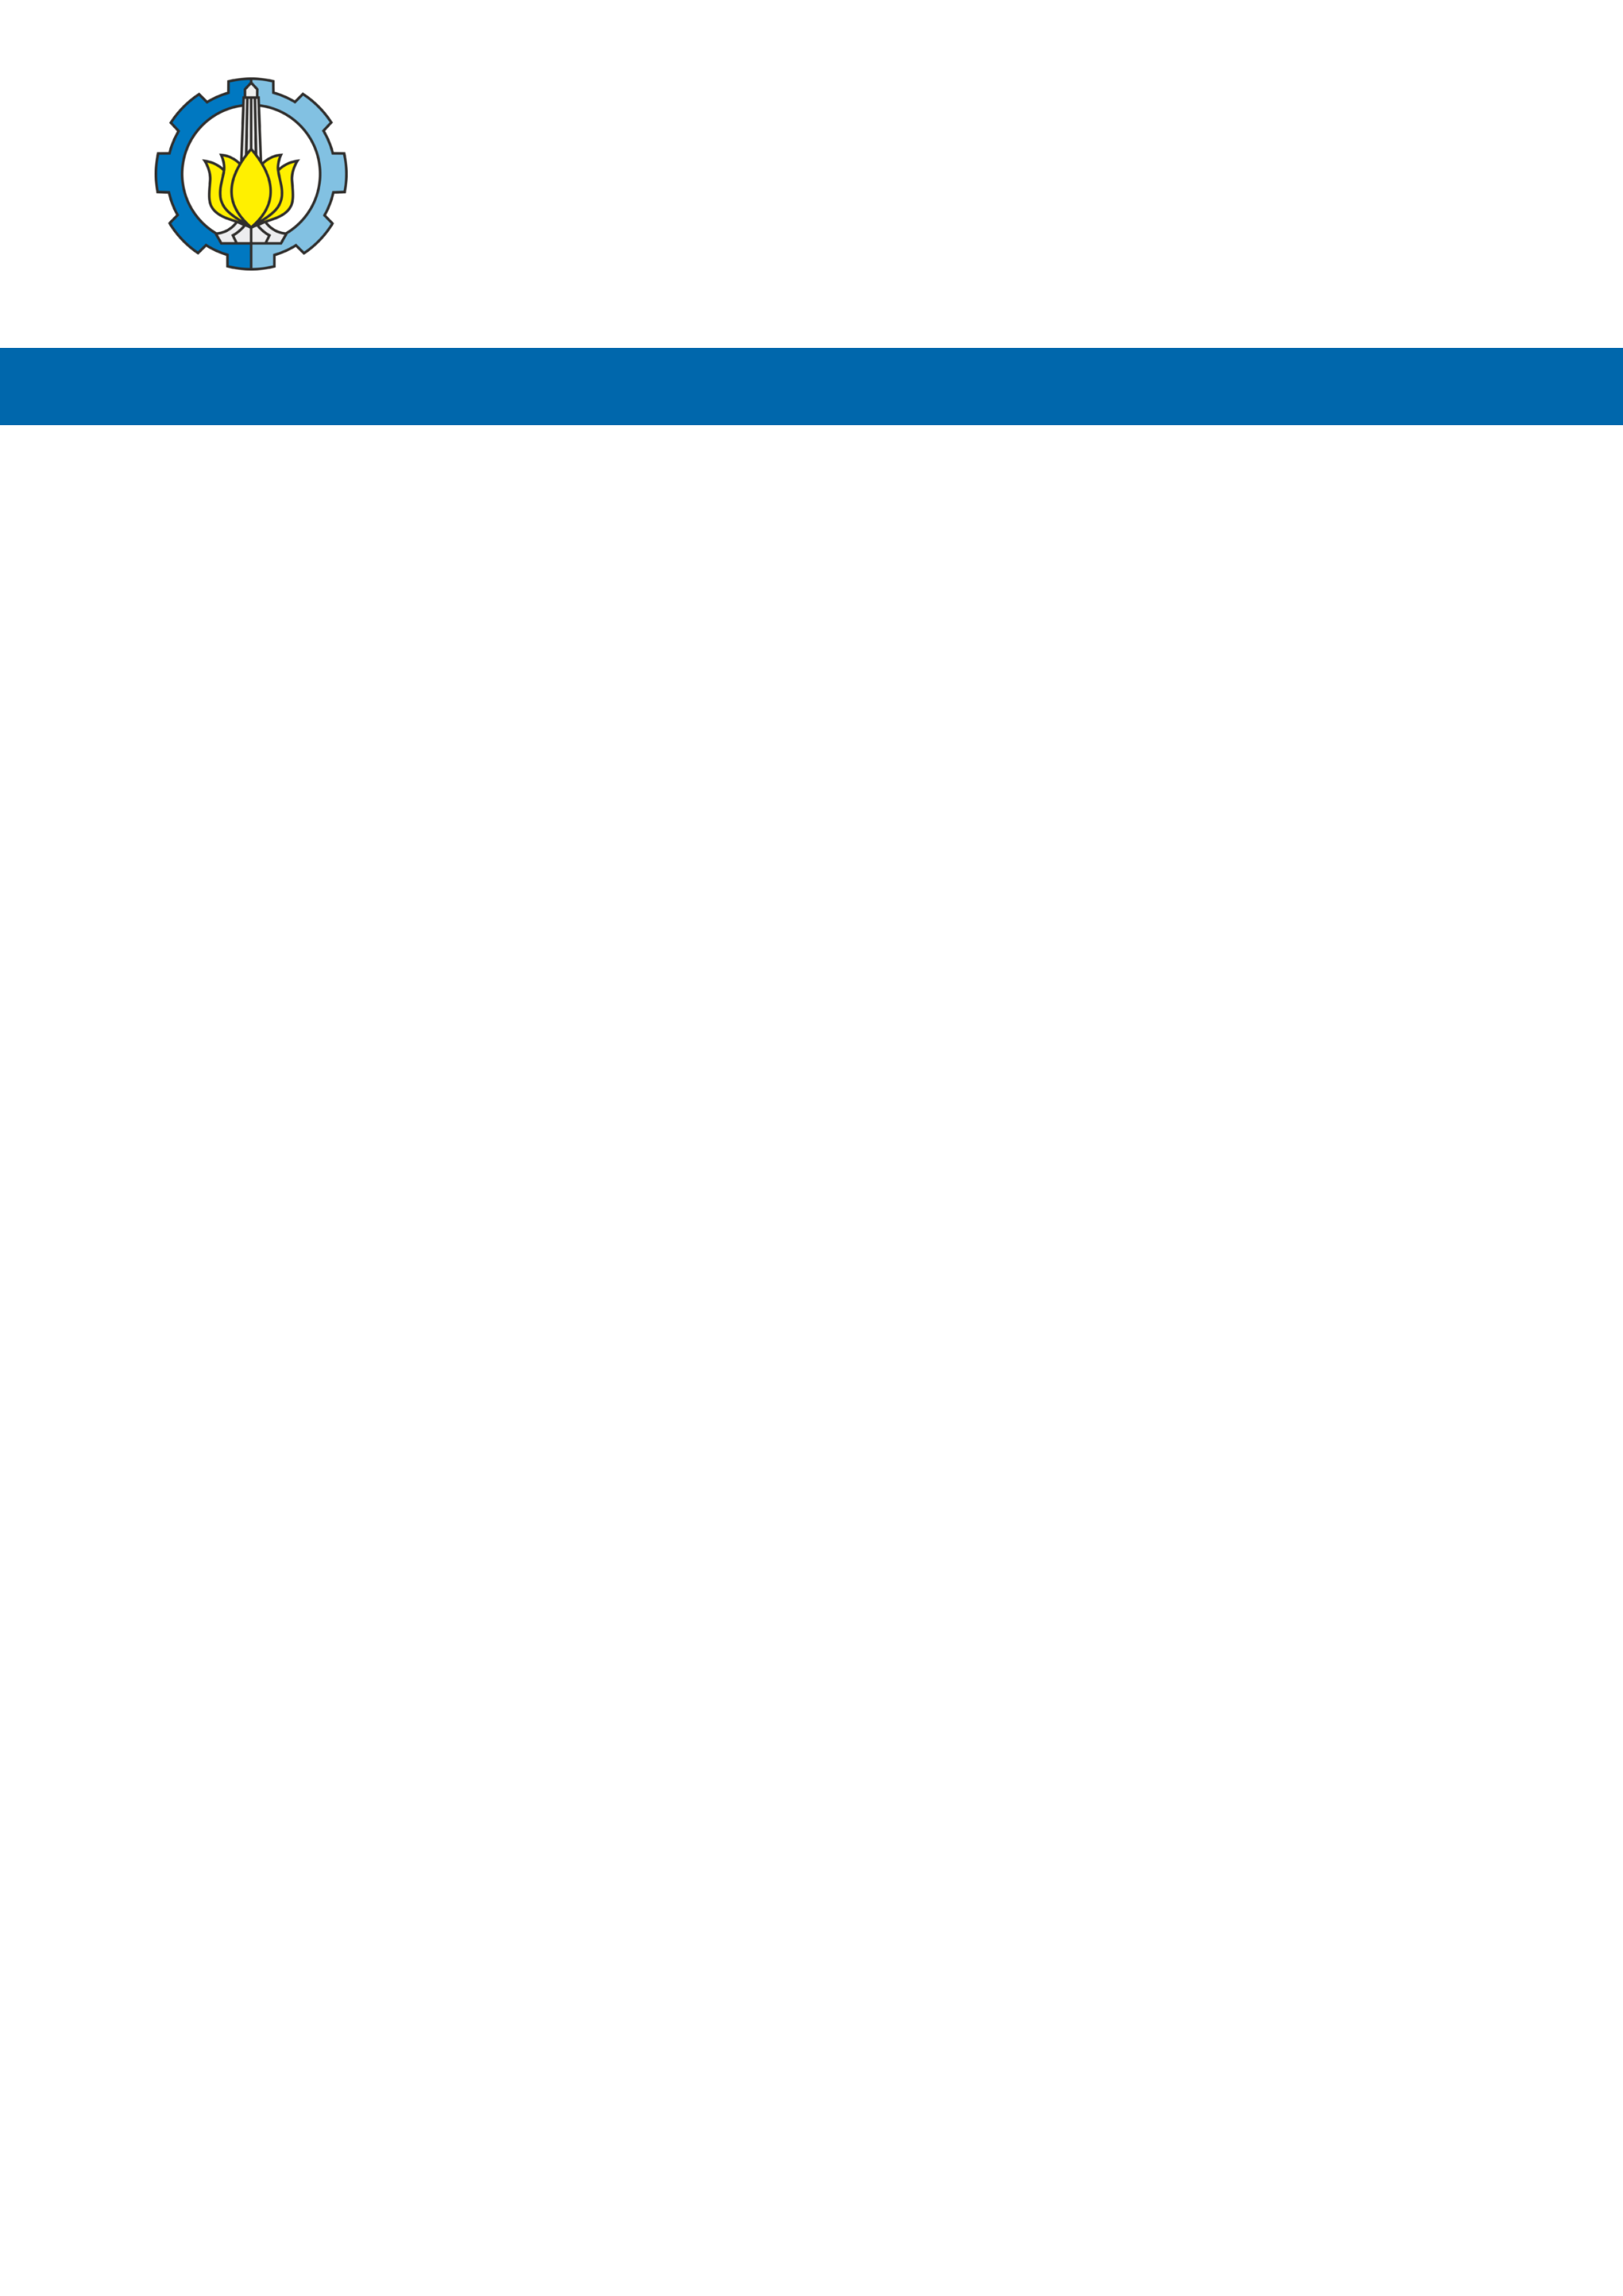
\includegraphics[width=\paperwidth,height=\paperheight]{Init/gambar/sampul-luar-tipis.png}
    }
  }
}

% Menyembunyikan nomor halaman
\thispagestyle{empty}

% Pengaturan margin untuk menyesuaikan konten sampul
\newgeometry{
  top=65mm,
  left=30mm,
  right=30mm,
  bottom=20mm
}

\begin{flushleft}

  % Pemilihan font sans serif
  \sffamily

  % Pemilihan font bold
  \fontseries{bx}
  \selectfont
  \begin{spacing}{1.5}
\begin{large}
  TUGAS AKHIR - \coursecode{}
\end{large}

\vspace{\fill}

\begin{spacing}{1.5}
  \begin{Large}
    \tatitle{}
  \end{Large}
\end{spacing}

\vspace{\fill}

\begin{large}
  \name{} \\
  \textmd{NRP \nrp{}}
\end{large}

\vspace{\fill}

\begin{large}
  \textmd{Dosen Pembimbing} \\
  \advisor{} \\
  \textmd{NIP \advisornip{}} \\
  \coadvisor{} \\
  \textmd{NIP \coadvisornip{}}
\end{large}

\vspace{\fill}

Program Studi Strata 1 (S1) \studyprogram{} \\

\mdseries

Departemen \department{} \\
Fakultas \faculty{} \\
Institut Teknologi Sepuluh Nopember

\place{} \\ \the\year{}

  \end{spacing}

\end{flushleft}

\restoregeometry

\clearpage
\cleardoublepage

% Sampul dalam Bahasa Inggris

\AddToShipoutPictureBG*{
  \AtPageLowerLeft{
    % Ubah nilai berikut jika posisi horizontal background tidak sesuai
    \hspace{-4mm}

    % Ubah nilai berikut jika posisi vertikal background tidak sesuai
    \raisebox{0mm}{
      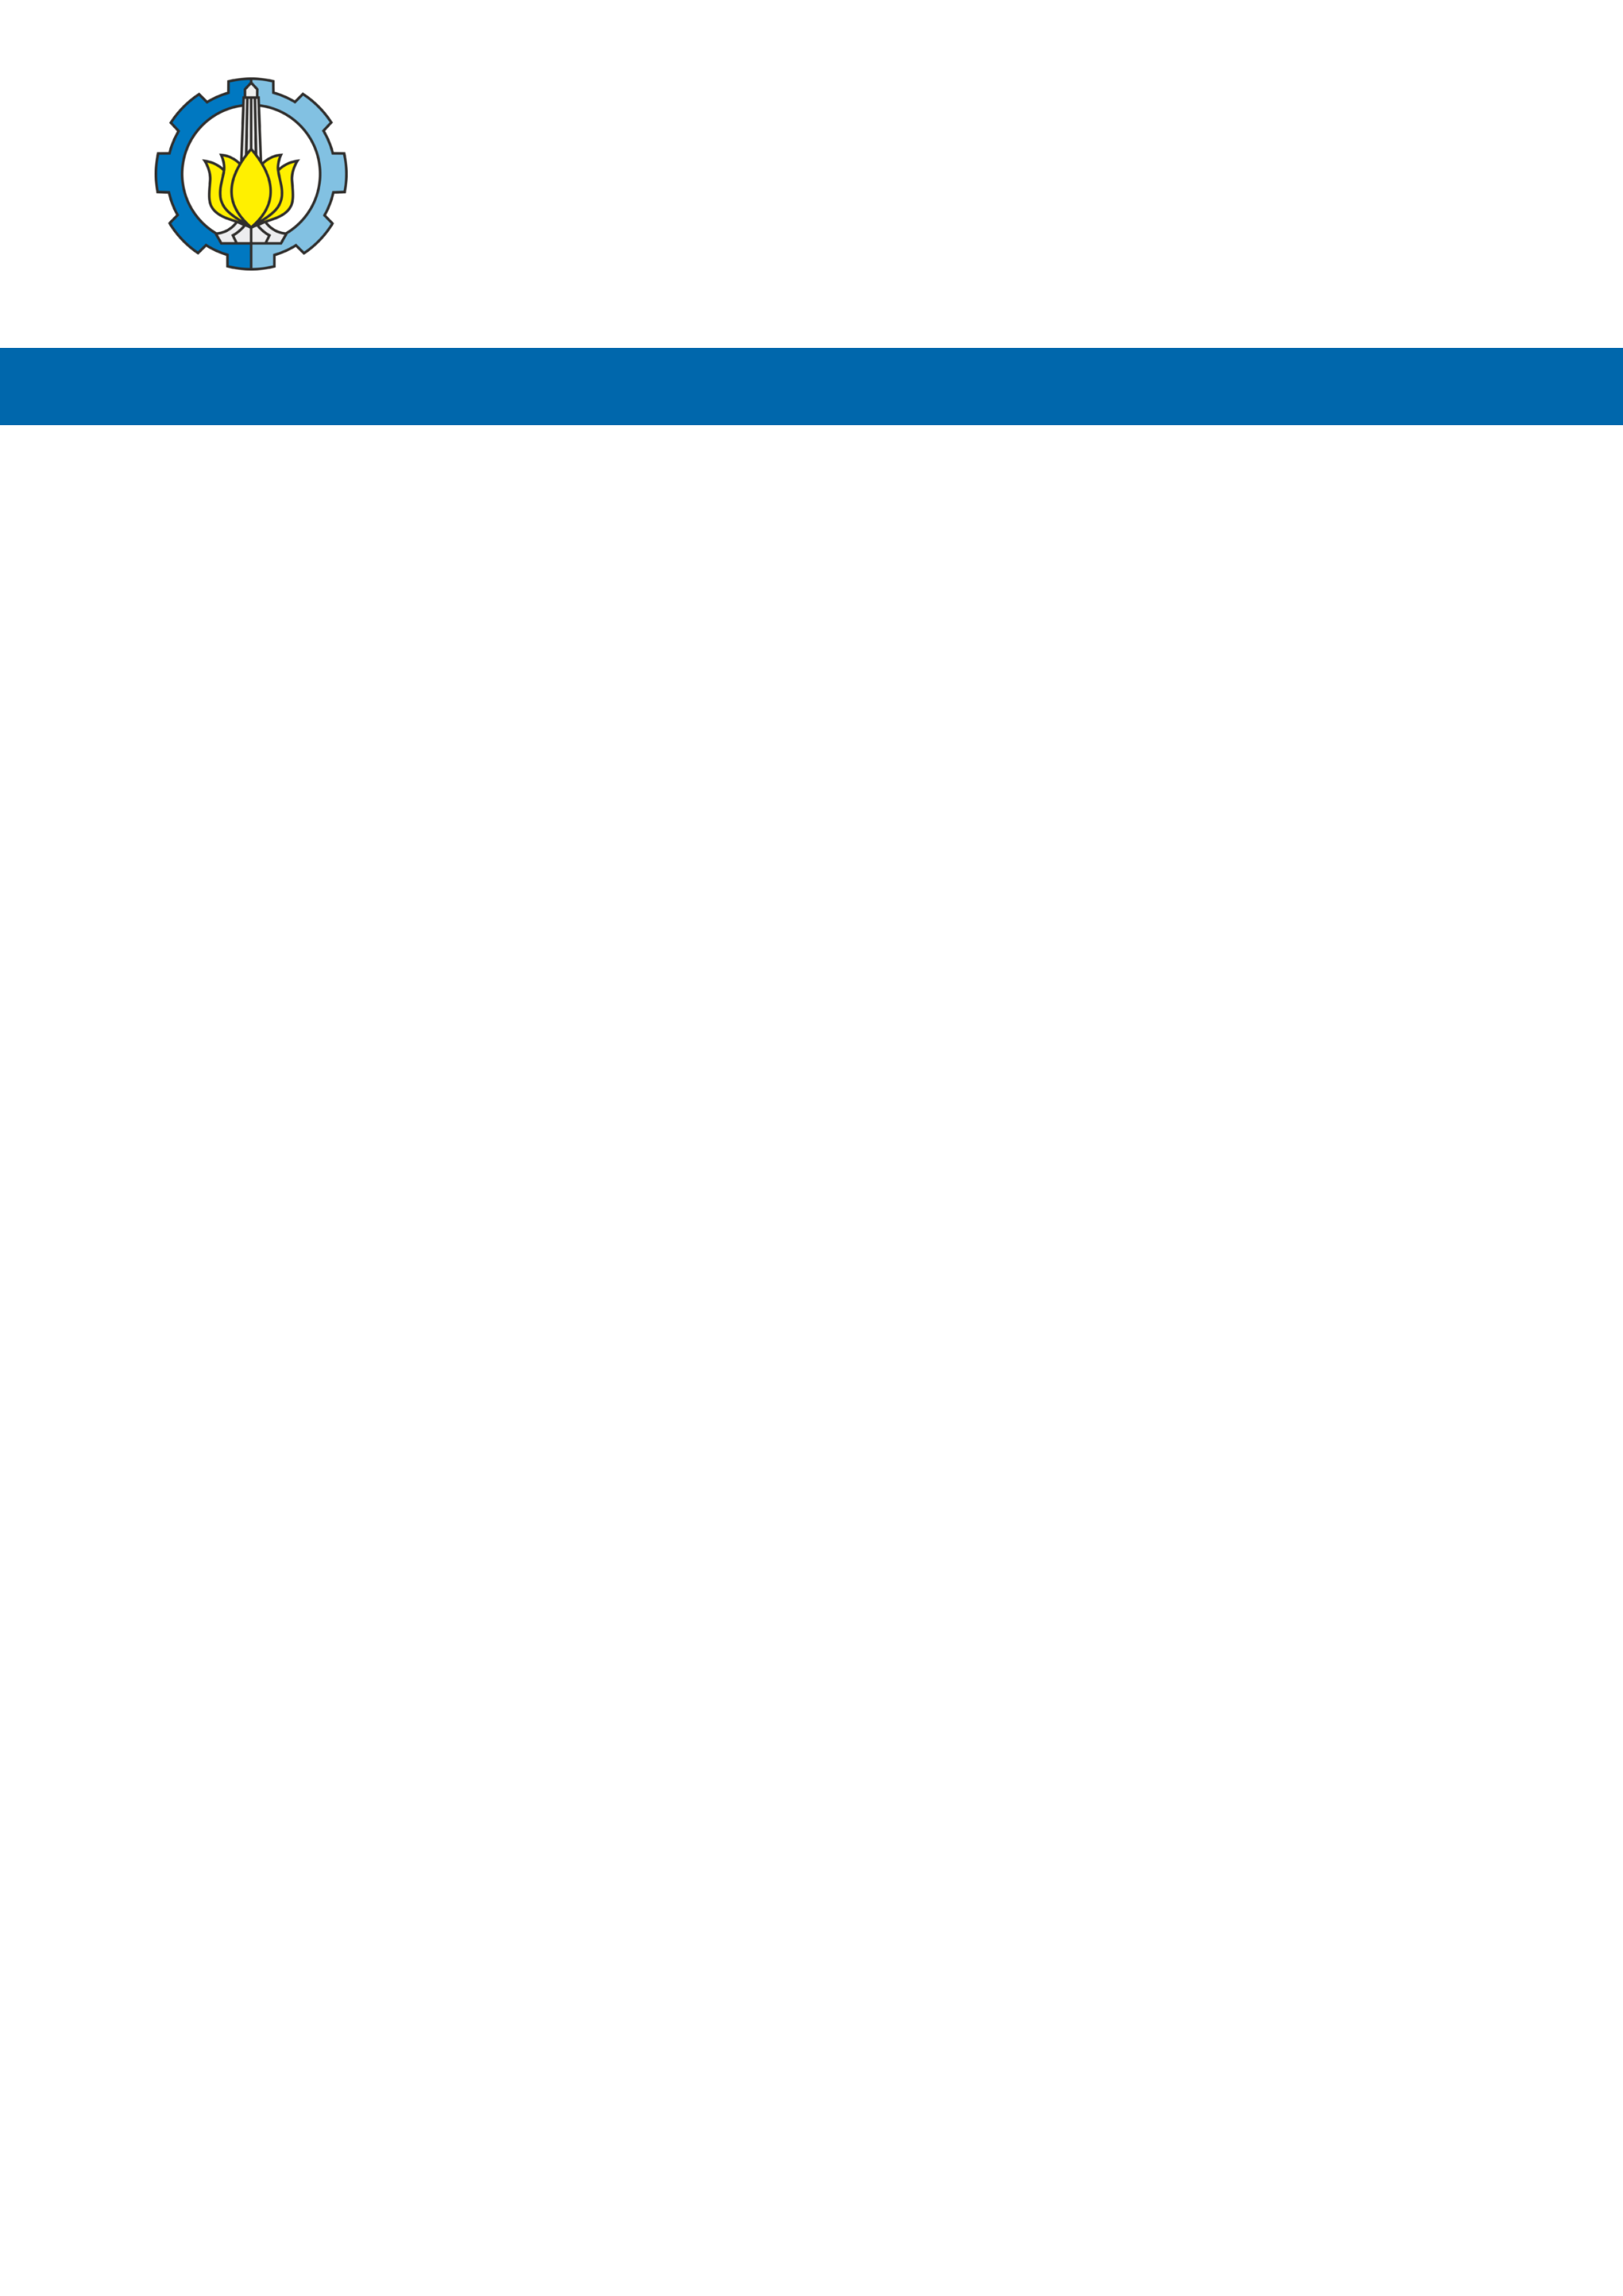
\includegraphics[width=\paperwidth,height=\paperheight]{Init/gambar/sampul-luar-tipis.png}
    }
  }
}

% Menyembunyikan nomor halaman
\thispagestyle{empty}

% Pengaturan margin untuk menyesuaikan konten sampul
\newgeometry{
  top=65mm,
  left=30mm,
  right=30mm,
  bottom=20mm
}

\begin{flushleft}

  % Pemilihan font sans serif
  \sffamily

  % Pemilihan font bold
  \fontseries{bx}
  \selectfont
  \begin{spacing}{1.5}
   \begin{large}
  FINAL PROJECT - \coursecode{}
\end{large}

\vspace{\fill}

\begin{spacing}{1.5}
  \begin{Large}
    \engtatitle{}
  \end{Large}
\end{spacing}

\vspace{\fill}

\begin{large}
  \name{} \\
  \textmd{NRP \nrp{}}
\end{large}

\vspace{\fill}

\begin{large}
  \textmd{Advisor} \\
  \advisor{} \\
  \textmd{NIP \advisornip{}} \\
  \coadvisor{} \\
  \textmd{NIP \coadvisornip{}}
\end{large}

\vspace{\fill}

Undergraduate Study Program of \engstudyprogram{} \\

\mdseries

Department of \engdepartment{} \\
Faculty of \engfaculty{} \\
Sepuluh Nopember Institute of Technology

\place{} \\ \the\year{}

  \end{spacing}

\end{flushleft}

\restoregeometry

\cleardoublepage

% Label tabel dan gambar dalam bahasa indonesia
\renewcommand{\figurename}{Gambar}
\renewcommand{\tablename}{Tabel}

% Pengaturan ukuran indentasi paragraf
\setlength{\parindent}{2em}

% Pengaturan ukuran spasi paragraf
\setlength{\parskip}{1ex}

% Lembar pengesahan
\begin{center}
  \large
  \textbf{LEMBAR PENGESAHAN}
\end{center}

% Menyembunyikan nomor halaman
\thispagestyle{empty}

\begin{center}
  \textbf{\tatitle{}}
\end{center}

\begingroup
% Pemilihan font ukuran small
\small

\begin{center}
  \textbf{TUGAS AKHIR}
  \\Diajukan untuk memenuhi salah satu syarat \\
  memperoleh gelar Sarjana Teknik pada \\
  Program Studi S-1 \studyprogram{} \\
  Departemen \department{} \\
  Fakultas \faculty{} \\
  Institut Teknologi Sepuluh Nopember
\end{center}

\begin{center}
  Oleh: \textbf{\name{}}
  \\NRP. \nrp{}
\end{center}

\begin{center}
  Disetujui oleh Tim Penguji Tugas Akhir:
\end{center}

\begingroup
% Menghilangkan padding
\setlength{\tabcolsep}{0pt}

\noindent
\begin{tabularx}{\textwidth}{X l}
  \advisor{}               & (Pembimbing I)                      \\
  NIP: \advisornip{}       &                                     \\
                           & ................................... \\
                           &                                     \\
                           &                                     \\
  \coadvisor{}             & (Pembimbing II)                     \\
  NIP: \coadvisornip{}     &                                     \\
                           & ................................... \\
                           &                                     \\
                           &                                     \\
  \examinerone{}.          & (Penguji I)                         \\
  NIP: \examineronenip{}   &                                     \\
                           & ................................... \\
                           &                                     \\
                           &                                     \\
  \examinertwo{}.          & (Penguji II)                        \\
  NIP: \examinertwonip{}   &                                     \\
                           & ................................... \\
                           &                                     \\
                           &                                     \\
\ifbool{bpenguji3}{
  \examinerthree{}.        & (Penguji III)                       \\
  NIP: \examinerthreenip{} &                                     \\
                          & ................................... \\
}


\end{tabularx}
\endgroup
\vspace{-1ex}
\begin{center}
  Mengetahui, \\
  Kepala Departemen \department{} \facultyshort{} - ITS\\

  \vspace{5ex}

  \underline{\headofdepartment{}.} \\
  NIP. \headofdepartmentnip{}
\end{center}
\vspace{-1ex}
\begin{center}
  \textbf{\MakeUppercase{\place{}}\\\MONTH{}, \the\year{}}
\end{center}
\endgroup

\cleardoublepage
\begin{center}
  \large
  \textbf{APPROVAL SHEET}
\end{center}

% Menyembunyikan nomor halaman
\thispagestyle{empty}

\begin{center}
  \textbf{\engtatitle{}}
\end{center}

\begingroup
% Pemilihan font ukuran small
\small

\begin{center}
  \textbf{FINAL PROJECT}
  \\Submitted to fulfill one of the requirements \\
  for obtaining a degree Bachelor of Engineering at \\
  Undergraduate Study Program of \engstudyprogram{} \\
  Department of \engdepartment{} \\
  Faculty of \engfaculty{} \\
  Sepuluh Nopember Institute of Technology
\end{center}

\begin{center}
  By: \textbf{\name{}}
  \\NRP. \nrp{}
\end{center}

\begin{center}
  Approved by Final Project Examiner Team:
\end{center}

\begingroup
% Menghilangkan padding
\setlength{\tabcolsep}{0pt}

\noindent
\begin{tabularx}{\textwidth}{X l}
  \advisor{}               & (Advisor I)                         \\
  NIP: \advisornip{}       &                                     \\
                           & ................................... \\
                           &                                     \\
                           &                                     \\
  \coadvisor{}             & (Co-Advisor II)                     \\
  NIP: \coadvisornip{}     &                                     \\
                           & ................................... \\
                           &                                     \\
                           &                                     \\
  \examinerone{}.          & (Examiner I)                        \\
  NIP: \examineronenip{}   &                                     \\
                           & ................................... \\
                           &                                     \\
                           &                                     \\
  \examinertwo{}.          & (Examiner II)                       \\
  NPP: \examinertwonip{}   &                                     \\
                           & ................................... \\
                           &                                     \\
                           &                                     \\
  \examinerthree{}.        & (Examiner III)                      \\
  NPP: \examinerthreenip{} &                                     \\
                           & ................................... \\
\end{tabularx}
\endgroup

\vspace{-1ex}
\begin{center}
  Acknowledged, \\
  Head of \engdepartment{} Department \engfacultyshort{} - ITS \\

  \vspace{8ex}

  \underline{\headofdepartment{}.} \\
  NIP. \headofdepartmentnip{}
\end{center}

\vspace{-1ex}
\begin{center}
  \textbf{\MakeUppercase{\place{}}\\\ENGMONTH{}, \the\year{}}
\end{center}
\endgroup
\cleardoublepage

% Pernyataan keaslian
\begin{center}
  \large
  \textbf{PERNYATAAN ORISINALITAS}
\end{center}

% Menyembunyikan nomor halaman
\thispagestyle{empty}

\vspace{2ex}

% Ubah paragraf-paragraf berikut sesuai dengan yang ingin diisi pada pernyataan keaslian

\noindent Yang bertanda tangan dibawah ini:

\noindent\begin{tabularx}{\textwidth}{l l X}
                         &   &                            \\
  Nama Mahasiswa / NRP   & : & \name{} / \nrp{}           \\
  Departemen             & : & \department{}              \\
  Dosen Pembimbing / NIP & : & \advisor{} / \advisornip{} \\
                         &   &                            \\
\end{tabularx}

Dengan ini menyatakan bahwa Tugas Akhir dengan judul "\tatitle{}" adalah hasil karya sendiri, berfsifat orisinal, dan ditulis dengan mengikuti kaidah penulisan ilmiah.

Bilamana di kemudian hari ditemukan ketidaksesuaian dengan pernyataan ini, maka saya bersedia menerima sanksi sesuai dengan ketentuan yang berlaku di Institut Teknologi Sepuluh Nopember.

\vspace{8ex}

\noindent\begin{tabularx}{\textwidth}{X l}
                     & \place{}, \MONTH{} \the\year{} \\
                     &                                   \\
  Mengetahui         &                                   \\
  Dosen Pembimbing   & Mahasiswa                         \\
                     &                                   \\
                     &                                   \\
                     &                                   \\
                     &                                   \\
                     &                                   \\
  \advisor{}         & \name{}                           \\
  NIP. \advisornip{} & NRP. \nrp{}                       \\
\end{tabularx}

\cleardoublepage
\begin{center}
  \large
  \textbf{STATEMENT OF ORIGINALITY}
\end{center}

% Menyembunyikan nomor halaman
\thispagestyle{empty}

\vspace{2ex}

% Ubah paragraf-paragraf berikut sesuai dengan yang ingin diisi pada pernyataan keaslian

\noindent The undersigned below:

\noindent\begin{tabularx}{\textwidth}{l l X}
                        &   &                            \\
  Name of student / NRP & : & \name{} / \nrp{}           \\
  Department            & : & \engdepartment{}           \\
  Advisor / NIP         & : & \advisor{} / \advisornip{} \\
                        &   &                            \\
\end{tabularx}

Hereby declared that the Final Project with the title of "\engtatitle{}" is the result of my own work, is original, and is written by following the rules of scientific writing.

If in future there is a discrepancy with this statement, then I am willing to accept sanctions in accordance with provisions that apply at Sepuluh Nopember Institute of Technology.

\vspace{8ex}

\noindent\begin{tabularx}{\textwidth}{X l}
                     & \place{}, \ENGMONTH{} \the\year{} \\
                     &                                   \\
  Acknowledged       &                                   \\
  Advisor            & Student                           \\
                     &                                   \\
                     &                                   \\
                     &                                   \\
                     &                                   \\
                     &                                   \\
  \advisor{}         & \name{}                           \\
  NIP. \advisornip{} & NRP. \nrp{}                       \\
\end{tabularx}
\cleardoublepage

% Nomor halaman pembuka dimulai dari sini
\pagenumbering{roman}

% Abstrak Bahasa Indonesia
\begin{center}
  \large\textbf{ABSTRAK}
\end{center}

\addcontentsline{toc}{chapter}{ABSTRAK}

\vspace{2ex}

\begingroup
% Menghilangkan padding
\setlength{\tabcolsep}{0pt}

\noindent
\begin{tabularx}{\textwidth}{l >{\centering}m{2em} X}
  Nama Mahasiswa    & : & \name{}         \\

  Judul Tugas Akhir & : & \tatitle{}      \\

  Pembimbing        & : & 1. \advisor{}   \\
                    &   & 2. \coadvisor{} \\
\end{tabularx} 
\endgroup

% Ubah paragraf berikut dengan abstrak dari tugas akhir
Peningkatan populasi penduduk di Indonesia secara langsung diikuti peningkatan resiko kemacetan dan kecelakaan lalu lintas. Dari data yang diperoleh, dapat diketahui bahwa dari tahun ke tahun jumlah kendaraan bermotor di Indonesia semakin meningkat diikuti dengan angka kecelakaan lalu lintas yang terjadi, dimana salah satu faktornya adalah pelanggaran batasan kecepatan. Untuk mengatasi masalah tersebut, dikemabangkan sebuah alat pemantauan dari udara dengan pemanfaatan \emph{drone} yang dapat melakukan perhitungan estimasi kecepatan kendaraan dengan didukung teknologi pengolahan citra video beserta program komputasi dalam menghitungnya. \emph{Drone} dimanfaatkan karena kemampuannya dalam melakukan pemantauan secara langsung dari udara dengan pengontrol jarak jauh. Sistem ini juga dikembangkan dengan berbasis Jetson Nano sehingga dapat dijalankan dimana saja. Metode yang dilakukan dalam pengolahan citra video ini adalah dengan memanfaatkan \emph{YOLOv8} untuk hasil yang akurat dan tepat.

% Ubah kata-kata berikut dengan kata kunci dari tugas akhir
Kata Kunci: pengawasan, Drone, stimasi kecepatan, Jetson Nano, YOLOv8

\cleardoublepage

% Abstrak Bahasa Inggris
\begin{center}
  \large\textbf{ABSTRACT}
\end{center}

\addcontentsline{toc}{chapter}{ABSTRACT}

\vspace{2ex}

\begingroup
% Menghilangkan padding
\setlength{\tabcolsep}{0pt}

\noindent
\begin{tabularx}{\textwidth}{l >{\centering}m{3em} X}
  \emph{Name}     & : & \name{}         \\

  \emph{Title}    & : & \engtatitle{}   \\

  \emph{Advisors} & : & 1. \advisor{}   \\
                  &   & 2. \coadvisor{} \\
\end{tabularx}
\endgroup

% Ubah paragraf berikut dengan abstrak dari tugas akhir dalam Bahasa Inggris
\emph{
  The increase in population in Indonesia is directly followed by an increase in the risk of traffic congestion and accidents. From the data obtained, it can be seen that from year to year the number of motorized vehicles in Indonesia is increasing, followed by the number of traffic accidents that occur, where one of the factors is speed limit violations. To overcome this problem, an aerial monitoring tool was developed using drones that can calculate vehicle speed estimates supported by video image processing technology and computing programs in their calculations. Drones are used because of their ability to monitor directly from the air with remote control. This system is also developed based on  Jetson Nano so that it can be run in anywhere. The method used in processing this video image is to utilize YOLOv8 for accurate and precise results.}

% Ubah kata-kata berikut dengan kata kunci dari tugas akhir dalam Bahasa Inggris
\emph{Keywords}: \emph{traffic control, Drone, speed estimation, jetson nano, YOLOv8}

\cleardoublepage

% Kata pengantar
\begin{center}
  \Large
  \textbf{KATA PENGANTAR}
\end{center}

\addcontentsline{toc}{chapter}{KATA PENGANTAR}

\vspace{2ex}

% Ubah paragraf-paragraf berikut dengan isi dari kata pengantar

Puji dan syukur kehadirat Tuhan Yang Maha Esa, atas segala rahmat dan karunia-Nya, sehingga penulis dapat menyelesaikan penelitian ini yang berjudul "\tatitle"

Penelitian ini disusun dalam rangka pemenuhan Tugas Akhir sebagai syarat kelulusan Mahasiswa ITS. Oleh karena itu, penulis mengucapkan banyak terima kasih kepada:

\begin{enumerate}[nolistsep]
  \item Bapak \advisor, selaku Kepala Departemen Teknik Komputer, Fakultas Teknologi Elektro dan Informatika Cerdas, Institut Teknologi Sepuluh Nopember yang juga menjadi Dosen Pembimbing I, serta Ibu \coadvisor, selaku Dosen Pembimbing II yang telah memberikan masukan dan arahan kepada penulis selama pengerjaan tugas akhir ini.
  \item Bapak-Ibu dosen pengajar Departemen Teknik Komputer, atas pelajaran dan ilmu yang telah diberikan kepada penulis selama masa perkuliahan.
  \item Kedua orang tua, kakak, keluarga, dan seorang perempuan terdekat yang tidak bisa disebut namanya yang selalu menemani dan memberi semangat dalam pengerjaan penulisan ini.
  \item Harist Ahmad Farhan, dan teman-teman yang lain, baik dari jurusan Teknik Komputer atau bukan, yang telah memberikan dukungan, motivasi, dan bantuan kepada penulis selama pengerjaan tugas akhir ini.
\end{enumerate}

Penelitian ini masih jauh dari kata sempurna, untuk itu penulis mengharapkan dengan segenap hati atas saran dan kritik yang membangun. Akhir kata, semoga penelitian ini dapat memberikan banyak manfaat untuk pembaca dan banyak pihak lainnya.

\begin{flushright}
  \begin{tabular}[b]{c}
    \place{}, \MONTH{} \the\year{} \\
    \\
    \\
    \\
    \\
    \name{}
  \end{tabular}
\end{flushright}

\cleardoublepage

% Daftar isi
\renewcommand*\contentsname{DAFTAR ISI}
\addcontentsline{toc}{chapter}{\contentsname}
\tableofcontents
\cleardoublepage

% Daftar gambar
\renewcommand*\listfigurename{DAFTAR GAMBAR}
\addcontentsline{toc}{chapter}{\listfigurename}
\listoffigures
\cleardoublepage

% Daftar tabel
\renewcommand*\listtablename{DAFTAR TABEL}
\addcontentsline{toc}{chapter}{\listtablename}
\listoftables
\cleardoublepage

% Nomor halaman isi dimulai dari sini
\pagenumbering{arabic} 

% Bab 1 pendahuluan

\begin{spacing}{1.2}
  \chapter{PENDAHULUAN}
\end{spacing}

\pagenumbering{arabic}
\vspace{4ex}

\section{Latar Belakang}
Peningkatan populasi di Indonesia selalu diikuti dengan peningkatan jumlah kendaraan. Menurut Data Korlantas Polri, terhitung pada bulan Agustus 2024, jumlah mobil pribadi mencapai 20,122,177 unit, dan jumlah sepeda motor mencapai 137,350,299 unit \cite{datakendaraan2024}. Apabila dilihat dari tahun-tahun sebelumnya, jumlah kendaraan yang telah beredar di Indonesia pada Februari 2023 mencapai 154,4 juta unit untuk semua jenis kendaraan bermotor yang aktif. Jumlah tersebut mencakup 127,9 juta unit sepeda motor, 19,17 juta unit mobil, dan sisanya terdapat angkutan barang serta mobil besar \cite{datakendaraan2023}. Dari angka tersebut membuktikan bahwa seiring bertambah tahun, jumlah kendaraan semakin meningkat sehingga menyebabkan kemacetan lalu lintas.

Kemacetan ini merupakan salah satu dampak yang terjadi. Peningkatan jumlah kendaraan juga memperbesar resiko kecelakaan lalu lintas yang menimbulkan korban, terutama menyebabkan cedera \cite{Ciss2019}. Faktor penyebab kecelakaan ini sangat banyak, salah satunya yang menjadi penyebab utama adalah kelalaian pengendara. Kelalaian ini disebabkan karena banyak pengendara yang mengendarai tanpa menaati aturan yang sudah ada, seperti batasan kecepatan pada beberapa titik jalan yang sudah diberi petunjuk \cite{jurnalspeed-roadsafety-relation}. Dikarenakan banyaknya populasi pengendara, diperlukan suatu inovasi yang dapat mengawasi kendaraan yang melintas. Maka dari itu, dikembangkan suatu alat yang diharapkan dapat menjadi solusi dari permasalahan diatas, yaitu dengan menggunakan \emph{drone}, dimana dapat dikendalikan sesuai dengan kebutuhan dan menjangkau lebih luas \cite{Kanistras2013}.

\emph{Drone} atau pesawat tanpa awak ini sudah banyak digunakan dalam pengaplikasian \emph{mapping} dan \emph{monitoring} dari atas dengan jangkauan yang luas. Pengendalian jarak jauh yang dapat merekam serta mengawasi dengan sistem video yang ditransmisikan dari kamera di \emph{drone} ke \emph{remote control}. Efektivitas yang dihasilkan dari penggunaan pesawat tanpa awak ini yang menjadi salah satu alasan dipilihnya \emph{drone}. Pemanfaatan pesawat tanpa awak ini sudah banyak dikembangkan dan diaplikasikan ke media pemanfaatan yang mana membutuhkan pengambilan data secara aerial, yaitu dari atas benda yang dijadikan objek data \cite{ZhangZhu2023}.

Dari keunggulan yang dimiliki oleh pesawat tanpa awak ini, tentu akan sangat membantu dalam menyelesaikan beberapa masalah yang terjadi di perkotaan. Dengan pemanfaatan \emph{drone} terhadap pengawasan kendaraan dari atas akan membuat efektivitas dalam pemantauan. Dengan ditambahnya fitur membaca kecepatan kendaraan dari data yang diambil kamera \emph{drone}. 

Pemrosesan citra video yang sudah lama diaplikasikan dan dikembangkan merupakan teknologi utama yang akan digunakan dalam membuat otomasi estimasi kecepatan kendaraan \cite{Tekalp1995}. Dengan teknologi pengidentifikasian objek, pembacaan pola, serta alat perhitungan dalam membaca data yang didapat. Didukung juga dengan program dalam menghitung kecepatan kendaraan terhadap video \emph{streaming} yang dihasilkan oleh \emph{drone}, dan penggunaan suatu perangkat untuk menjalankan program komputasi tersebut dimana saja hanya dengan perlu menghubungkan antar perangkat melalui sebuah protokol.

Teknologi pemrosesan citra ini menjadi salah satu teknologi yang semakin banyak digunakan karena kebutuhan akan otomasi untuk sebuah proses sehingga didapatkan efisiensi terhadap sistem. Sebagai contoh, diperlukan pengawasan yang efisien dan dapat menjangkau tempat yang lebih luas tanpa perlu pemasangan alat pengawasan terlebih dahulu. Maka, dalam pengawasan lalu lintas yang dapat menghitung kecepatan kendaraan yang melintas diperlukan deteksi objek sehingga pemrosesan citra ini dapat diaplikasikan dalam pengembangan sistem estimasi kecepatan dengan \emph{drone} pada penelitian ini.

\section{Rumusan Masalah}
Berdasarkan latar belakang tersebut, jumlah kendaraan terus meningkat sehingga dibutuhkan pengawasan lalu lintas yang tidak perlu membangun alat pengawasan di banyak tempat. Belum meratanya sistem pengawasan lalu lintas yang dapat membaca kecepatan kendaraan melintas menjadi permasalahan sehingga fleksibilitas dibutuhkan untuk melakukan pengawasan tersebut.

\section{Batasan Masalah}
Penelitian ini berfokus pada estimasi kecepatan kendaraan yang ada di jalan raya dengan dilakukan pendeteksian kendaraan yang melintas. Sistem dapat mendeteksi kendaraan pada kondisi siang hari dan malam hari. Pendeteksian objek kendaraan menggunakan pemrosesan citra sehingga dapat dihitung kecepatannya. Implementasi sistem ini menggunakan \emph{edge device}, yaitu Jetson Nano. Penggunaan sistem tidak dapat dilakukan terlalu lama karena keterbatasan perangkat dan baterai yang dimiliki \emph{drone}.

\section{Tujuan}
Tujuan dilakukan penelitian ini adalah untuk peningkatan efektivitas dalam pemantauan lalu lintas dengan pemanfaatan \emph{drone} yang menghasilkan estimasi kecepatan kendaraan yang melintas. Maka, diharapkan dapat membantu satuan otoritas setempat dalam mengawasi lalu lintas dengan mudah dan fleksibel. Dengan penggunaan teknologi pengolahan citra video yang didukung Jetson Nano sehingga dapat melakukan perhitungan dengan alat yang \emph{portable} yaitu dapat dimana saja dalam menjalankan komputasinya.
 
\section{Manfaat}
Berdasarkan hal-hal yang telah dijelaskan diatas, penelitian tugas akhir ini memiliki beberapa manfaat yang dihasilkan, antara lain:
\begin{enumerate}
    \item Hasil perhitungan kecepatan kendaraan yang melintas secara langsung.
    \item Meningkatkan efektivitas pengawasan dan pemantauan lalu lintas yang berbasis perangkat \emph{edge} sehingga dapat digunakan \emph{portable}, dan dapat diterapkan di berbagai lokasi.
    \item Memberikan kontribusi terhadap pengembangan sistem pemantauan lalu lintas berbasis \emph{drone}, yang dapat menjadi alternatif pemantauan dengan biaya lebih rendah dan kemampuan mobilitas tinggi.
\end{enumerate}

\section{Sistematika Penulisan}
Laporan penelitian tugas akhir ini disusun secara sistematis dan terstruktur sehingga mudah dipahami dan dipelajari oleh pembaca. Alur sistematika penulisan laporan penelitian ini, yaitu:

\begin{enumerate}
    \item \textbf{BAB I Pendahuluan} \\
    Bab ini berisi tentang uraian latar belakang, permasalahan, penegasan dan alasan pemilihan judul, sistematika laporan, tujuan, dan manfaat.
    
    \item \textbf{BAB II Tinjauan Pustaka} \\
    Bab ini berisi tentang uraian penelitian terdahulu dan teori yang berkaitan maupun yang digunakan pada penelitian ini secara sistematis. Teori-teori yang disebutkan digunakan sebagai dasar dalam penelitian ini antara lain informasi tentang deep learning, drone, kamera, serta teori penunjang lainnya.
    
    \item \textbf{BAB III Desain dan Implementasi Sistem} \\
    Bab ini berisi tentang perancangan dan implementasi sistem yang digunakan dalam penelitian ini. Penjelasan tentang perangkat keras, dan perangkat lunak yang digunakan, serta alur kerja sistem yang digunakan.
    
    \item \textbf{BAB IV Pengujian, Analisis, dan Perbandingan} \\
    Bab ini berisi tentang tahap pengujian dari penelitian yang dilakukan terhadap data yang sebelumnya telah dikumpulkan. Pada bab ini juga ditampilkan visualisasi hasil pengujian dan perbandingan dengan penelitian terdahulu yang terkait.
    
    \item \textbf{BAB V Penutup} \\
    Bab ini berisi tentang kesimpulan dari penelitian yang telah dilakukan, saran, dan rekomendasi untuk penelitian selanjutnya.
\end{enumerate}


\cleardoublepage

\begin{spacing}{1.2}
	\chapter{TINJAUAN PUSTAKA}
\end{spacing}
  
\vspace{4ex}

\section{Hasil Penelitian Terdahulu}
Pengerjaan penelitian ini juga dipengaruhi adanya beberapa hasil penelitian terdahulu yang terkait, sebagai berikut:

\subsection{Perhitungan Kecepatan Kendaraan Menggunakan Drone Bergerak dengan Metode Deep Learning}
\label{subsec:Iqbal2024}
Penelitian ini dikembangkan oleh Iqbal Fatchurozi, untuk penyelesaian Tugas Akhir. Penulis melakukan penelitian terkait penggunaan \emph{drone} dalam pengawasan lalu lintas. Implementasi pengolahan citra video untuk melakukan perhitungan kecepatan kendaraan dari atas menggunakan \emph{drone} yang dilakukan dengan komputer untuk komputasinya. Metode deteksi objek yang digunakan adalah YOLOv8 dengan menggunakan streamlit untuk mengirimkan video ke komputer server sebagai tempat pemrosesan data \cite{Iqbal2024}. 

\subsection{Vehicle Tracking and Speed Estimation from Unmanned Aerial Vehicles Using Segmentation-Initialised Trackers}
\label{subsec:Tilon2023}
Pendekatan umum dalam estimasi kecepatan kendaraan berbasis \emph{Unmanned Aerial Vehicle} (UAV) menggunakan deteksi objek seperti \emph{YOLOv4} yang dikombinasikan dengan pelacak seperti \emph{DeepSORT}. Meskipun akurat, metode ini kurang efisien untuk \emph{edge device} karena beban komputasi yang tinggi. Sebagai alternatif, digunakan pelacak \emph{MOSSE} yang ringan, sementara peneliti yang lain menunjukkan pentingnya jarak UAV terhadap objek dalam sistem pelacakan.

Menanggapi keterbatasan tersebut, Tilon dan Nex (2023) mengembangkan metode pelacakan berbasis segmentasi menggunakan model \emph{CABiNet}. Dengan inisialisasi pelacakan dari hasil segmentasi, metode ini mampu berjalan pada \emph{edge device} seperti \emph{Jetson Xavier NX} dan menghasilkan \emph{MOTP} sebesar 0{,}872, lebih tinggi dibandingkan metode berbasis deteksi objek. Pendekatan ini menawarkan efisiensi serta fleksibilitas dalam menghasilkan informasi semantik untuk pemantauan infrastruktur \cite{Tilon2023}.

\subsection{Automatic Vehicle Speed Estimation Method for Unmanned Aerial Vehicle Images}
Penelitian yang telah dilakukan oleh Hao Long, Yi-Nung, dan rekan menghasilkan metode otomatis untuk mendeteksi dan menghasilkan estimasi kecepatan kendaraan melalui citra udara dari UAV. Metode yang digunakan meliputi trannsformasi warna dengan HSV, meminimalisir bayangan, dan memisahkan objek deteksi dari latar menggunakan perbedaan temporal. Proses estimasi kecepatan yang digunakan adalah menghitung jarak perpindahan objeknya dalam satuan piksel, yang didukung dengan lebar jalan sebagai skala konversi jarak \cite{auto-vehicle-speed-uav-img}.

\subsection{A novel vehicle tracking and speed estimation with varying UAV altitude and video resolution}
Jurnal ini membahas perihal metode deteksi kendaraan dan estimasi kecepatan menggunakan video udara dari atas dengan variasi ketinggian yang dihasilkan dari \emph{Unmanned Aerial Vehicle} beserta resolusi video yang dilakukan oleh Yuqing Chen, Dongyang Zhao, dan rekan. Metode deteksi yang digunakan adalah YOLOv3, kemudian untuk estimasi kecepatannya menggunakan pemetaan piksel ke jarak nyata secara eksponensial. Pendekatan yang dilakukan untuk estimasi kecepatan kecepatannya ialah memanfaatkan hubungan eksponensial yang dihasilkan dari \emph{fitting} data antara jarak piksel dengan jarak aktual yang didukung \emph{least square} sehingga tidak diperlukan kalibrasi kamera yangg kompleks \cite{novel-vehicle-tracking}.

\subsection{Real-Time Traffic Flow Parameter Estimation From UAV Video Based on Ensemble Classifier and Optical Flow}
Jurnal yang ditulis oleh Zhibin Li, Jinjun Tang, dan rekan berisi tentang pembahasan untuk menghitung perkiraan aliran lalu lintas seperti kecepatan, kepadatan, dan volume menggunakan video dari \emph{UAV}. Klasifikasi \emph{Haar cascade} digunakan untuk menghitung ROI \emph{Region of Interest}, kemudian CNN sebagai klasifikasi akhir dalam deteksi kendaraan. Estimasi \emph{motion} dilakukan dengan \emph{optical flow} untuk mengukur perpindahan kendaraan dan latar belakang secara terpisah. Lalu, untuk memperkirakan parameter aliran lalu lintas digunakan informasi dari deteksi dan estimasi \emph{motion} untuk menghitung parameternya seperti kecepatan, kepadata, dan volume \cite{realtime-trafficflow-estimation}.

\subsection{AI-Powered Automated Road Damage Detection Using UAV Images and Deep Learning}
Penelitian ini mengembangkan sistem deteksi kerusakan jalan otomatis dengan memanfaatkan \emph{Unmanned Aerial Vehicle} (UAV) dan model deep learning berbasis CNN, khususnya varian YOLO (v5, v7, v8). Citra udara resolusi tinggi yang diambil dari berbagai sudut dan ketinggian diproses lebih dulu, meliputi pengurangan noise, dan peningkatan kontras sebelum dianalisis oleh model yang dievaluasi menggunakan metrik mAP, presisi, dan recall untuk memastikan keakuratannya. Hasil pengujian menunjukkan YOLOv8 unggul dalam akurasi dan kecepatan inferensi secara \emph{real time}, dan hasil deteksi langsung diintegrasikan ke dalam sistem GIS untuk mempermudah pemetaan serta penentuan prioritas perbaikan. Dengan demikian, pendekatan ini mempercepat inspeksi, meminimalkan kesalahan manusia, dan memungkinkan pemantauan skala besar secara berkelanjutan, sehingga perbaikan dapat dilakukan tepat waktu dan umur infrastruktur jalan pun terjaga. Untuk kedepannya, cakupan penelitian akan diperluas dengan menambah dataset, menerapkan transfer learning, serta menggunakan metode \emph{ensemble} untuk meningkatkan daya tahan dan akurasi model \cite{bujji-ai}.

\subsection{Efficient Roundabout Supervision: Real-Time Vehicle Detection and Tracking on Nvidia Jetson Nano}
Penelitian ini dikembangkan dengan menggunakan \emph{edge device} yaitu Jetson Nano, dimana pendekatan deteksi kendaraan yang digunakan adalah \emph{YOLOv7-tiny} serta \emph{Deep SORT} untuk pelacakan. Imane Elmanaa yang merupakan penulis dari jurnal ini membahas perihal pendeteksian, pelacakan, perhitungan berbagai jenis kendaraan secara \emph{real-time} pada persimpangan di negara Maroko guna mendukung perencanaan infrastruktur \cite{efficient-roundabout-supervision}.

\subsection{Perancangan Sistem Pengukur Kecepatan Kendaraan Berbasis Kamera Menggunakan Algoritma YOLO}
Penelitian yang dilakukan oleh Zikri Giarida dan Perani Rosyani membahas perancangan sistem untuk mengukur kecepatan kendaraan berbasis kamera menggunakan YOLO. YOLO disini digunakan untuk mendeteksi kendaraan yang lewat. Proses kalibrasi dilakukan dengan menentukan koordinat dari video yang disesuaikan dengan jarak aktual di dunia nyata dengan garis pengukuran. Kemudian, kecepatan kendaraan dihitung berdasarkan waktu yang dibutuhkan untuk melewati area pengukuran dengan menggunakan rumus jarak \emph{euclidean} yang dikonversikan ke kilometer per jam \cite{perancangan-sistem-pengukur-kecepatan}.

\section{Landasan Teori}
Konsep dasar atau teori yang digunakan dalam penelitian ini tercantum pada sub-bab dibawah ini:

\subsection{DJI Phantom 4 Pro}
DJI Phantom 4 Pro merupakan salah satu model \emph{drone} keluaran DJI, yang merupakan perusahaan besar dimana berfokus pada pengembangan alat teknologi, salah satunya yang terkenal adalah produk \emph{drone}nya. Phantom 4 Pro memiliki kelebihan dibanding versi sebelumnya dimana dia sudah mampu menghindari tabrakan karena adanya \emph{rear-facing obstacle sensing system} di bagian belakang, serta sensor inframerah di bagian kiri dan kanan. \emph{Drone} ini memiliki resistansi terhadap angin dengan maksimum sebesar 10m/s, dan dapat diterbangkan selama kurang lebih 30 menit \cite{djiphantom4pro}.

Kamera gimbal yang digunakan pada \emph{drone} ini memiliki piksel sebesar 20MP. Maksimum kualitas yang dapat diatur pada kamera ini sebesar 4K 60p (H.264) dan 4K 30p (H.265) dengan maksimal \emph{bitrate} sebesar 100Mbps. Hasil rekaman maupun tangkapan layar dari kamera DJI Phantom 4 Pro dapat disimpan dengan \emph{Micro SD Card} yang dihubungkan ke \emph{drone}. Terdapat juga \emph{controller} yang dapat dihubungkan dengan USB atau HDMI melalui perangkat keras seperti, \emph{smartphone} \cite{djiphantom4pro}. 

\subsection{Nvidia Jetson Nano \emph{Developer Kit}}

Jetson Nano Developer Kit adalah sebuah komputer mini berbasis AI yang dirancang oleh NVIDIA untuk memberikan kemampuan komputasi tingkat tinggi dalam ukuran kecil dan konsumsi daya yang rendah. Perangkat ini ditujukan bagi para pengembang, pelajar, dan maker yang ingin mengeksplorasi aplikasi kecerdasan buatan, seperti visi komputer, robotika, dan sistem tertanam berbasis AI. Jetson Nano dilengkapi dengan GPU NVIDIA Maxwell 128-core, CPU quad-core ARM Cortex-A57, dan RAM LPDDR4 4GB, yang secara keseluruhan cukup untuk menjalankan model \emph{deep learning} modern secara \emph{real-time}. Didukung oleh JetPack SDK, Jetson Nano dapat menjalankan sistem operasi berbasis Linux lengkap dengan pustaka-pustaka seperti CUDA, cuDNN, TensorRT, OpenCV, dan lainnya yang dibutuhkan untuk pengembangan aplikasi AI.

Sebelum digunakan, Jetson Nano \emph{Developer Kit} memerlukan instalasi sistem operasi ke dalam kartu microSD yang akan berfungsi sebagai media penyimpanan utama. NVIDIA menyediakan \emph{image} OS yang sudah terintegrasi dengan JetPack dan dapat diunduh melalui situs resminya. Pengguna cukup menulis \emph{image} tersebut ke dalam kartu microSD UHS-1 berkapasitas minimal 16GB menggunakan alat seperti Balena Etcher. Setelah kartu dimasukkan, Jetson Nano dapat dihubungkan dengan periferal seperti monitor HDMI atau \emph{display port}, mouse dan keyboard USB, serta jaringan \emph{Ethernet}. Daya untuk perangkat ini dapat disuplai melalui \emph{port} micro-USB 5V/2A atau dengan adaptor DC \emph{barrel jack} 5V/4A untuk performa maksimal. Setelah semua terhubung, sistem akan menyala otomatis dan pengguna akan diarahkan ke proses konfigurasi awal melalui antarmuka grafis \cite{nvidia2020nano}.

Jetson Nano juga dilengkapi dengan berbagai antarmuka I/O yang memungkinkan fleksibilitas tinggi dalam pengembangan proyek. Terdapat empat \emph{port} USB 3.0 untuk periferal tambahan, slot kamera CSI untuk modul kamera seperti Raspberry Pi Camera V2, serta \emph{header} GPIO 40-pin yang kompatibel dengan Raspberry Pi, memungkinkan integrasi berbagai sensor dan aktuator. Di sisi jaringan, tersedia slot M.2 Key E untuk modul Wi-Fi tambahan jika diperlukan. Selain itu, tersedia juga antarmuka seperti I2C, I2S, UART, dan SPI untuk keperluan komunikasi antar perangkat. Dengan semua fitur ini, Jetson Nano menjadi platform yang sangat cocok untuk proyek AI edge computing yang membutuhkan pemrosesan cepat secara lokal, tanpa bergantung pada \emph{cloud}. Ketersediaan dokumentasi resmi dan komunitas pengembang yang luas juga semakin mendukung pengguna dalam eksplorasi dan implementasi solusi berbasis AI \cite{hanifah2022perbandingan}.


\subsection{\emph{Real-Time Messaging Protocol}(RTMP)}
\emph{Real-Time Messaging Protocol} (RTMP) merupakan salah satu protokol yang banyak digunakan dalam sistem \emph{streaming} video dan audio secara langsung melalui jaringan internet. RTMP awalnya dikembangkan oleh Macromedia (sekarang Adobe) untuk mengoptimalkan pengiriman data multimedia antara server dan klien secara real-time. Protokol ini mendukung transmisi data secara kontinu dengan latensi rendah, sehingga sangat cocok untuk aplikasi \emph{live streaming} seperti webinar, siaran langsung, dan konferensi video.

Keunggulan utama RTMP terletak pada latensi yang rendah, koneksi yang persisten, serta kemudahan integrasi dengan berbagai perangkat lunak encoder modern. RTMP juga mendukung metode \emph{push} dan \emph{pull} dalam transfer data, yang memberikan fleksibilitas dalam pengelolaan aliran video langsung. Selain itu, RTMP banyak digunakan sebagai protokol \emph{ingest}, yaitu proses pengiriman data dari encoder ke server sebelum didistribusikan ke pengguna akhir menggunakan protokol lain seperti HLS atau DASH \cite{dyte2023rtmp}.

Implementasi server streaming berbasis RTMP dapat dilakukan menggunakan perangkat lunak \emph{open-source} seperti Nginx-RTMP. Dengan konfigurasi yang tepat, satu server RTMP dapat menerima satu aliran video dari \emph{encoder} dan mendistribusikannya ke banyak platform secara simultan (\emph{multi-streaming}), sehingga sangat efisien dalam penggunaan \emph{bandwidth} dan sumber daya server. Hal ini sangat bermanfaat bagi kreator konten yang ingin melakukan siaran langsung ke beberapa platform sekaligus tanpa perlu mengirimkan \emph{stream} terpisah untuk setiap layanan \cite{linode2021rtmp}.

\subsection{\emph{Deep Learning}}
Di \emph{deep neural network} layer masukan menerima data, yang melewati lapisan tersembunyi yang mengubah data menggunakan fungsi non-linier. 

\begin{figure} [H] \centering
  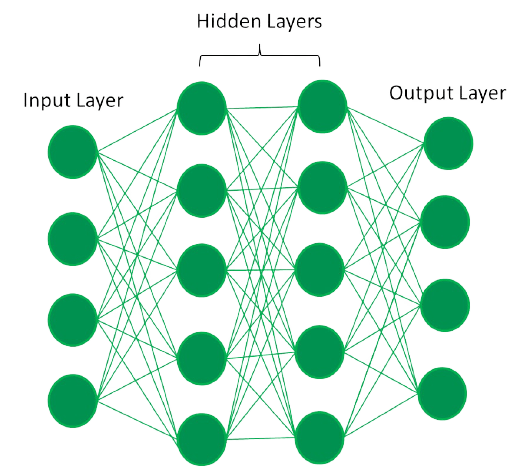
\includegraphics[scale=0.5]{bab2/deeplearning.png}
  \caption{\emph{Deep Neural Network} \cite{deeplearningimg}}
  \label{fig:neuralnetwork}
\end{figure}

\emph{Deep learning} dibangun di atas konsep \emph{artificial neural network} dengan menyusun banyak lapisan neuron yang saling terhubung untuk mempelajari representasi fitur secara hirarki. Setiap lapisan melakukan transformasi afine yang diikuti fungsi aktivasi nonlinier seperti \emph{ReLU} dan \emph{sigmoid} sehingga model mampu mengekspresikan fungsi-fungsi kompleks. Pelatihan jaringan ini memanfaatkan algoritma \emph{backpropagation} untuk menghitung gradien secara efisien, yang kemudian dioptimalkan dengan metode \emph{gradient descent} mulai dari \emph{batch} dan \emph{mini-batch} hingga varian canggih seperti \emph{momentum} dan \emph{Adam}. Untuk menjaga kestabilan dan mempercepat proses konvergensi, diaplikasikan juga teknik seperti inisialisasi bobot yang tepat, \emph{batch normalization}, \emph{dropout}, serta penjadwalan laju pembelajaran.

Selain jaringan \emph{feedforward}, berbagai arsitektur khusus dikembangkan sesuai karakteristik data. \emph{Convolutional Neural Network} (\emph{CNN}) memanfaatkan lapisan konvolusi dan pooling untuk mengekstrak pola spasial dalam citra, membangun peta fitur bertingkat sebelum tahap klasifikasi atau regresi. Sementara itu, \emph{Recurrent Neural Network} (RNN) dan varian berpintu seperti LSTM dan GRU dirancang untuk memproses data sekuensial seperti teks atau sinyal waktu dengan menyimpan jejak konteks antar langkah waktu melalui status tersembunyi. Di sisi tak terawasi, \emph{autoencoder} mengompresi input ke \emph{embedding} berdimensi rendah dan merekonstruksi kembali keluaran, berguna untuk deteksi anomali dan reduksi dimensi. Melalui TensorFlow 2 dan Keras, praktisi dapat mengombinasikan lapisan-lapisan ini untuk merancang model deep learning yang sesuai beragam aplikasi \cite{Geron2019}.

Dalam beberapa tahun terakhir, \textit{deep learning} telah mengalami perkembangan signifikan berkat kemunculan arsitektur baru yang lebih efisien dan fleksibel, seperti transformer. Model ini mengandalkan mekanisme \textit{self-attention} untuk memahami dependensi global dalam data sekuensial tanpa perlu pemrosesan sekuensial seperti pada RNN. Dengan pendekatan ini, model seperti BERT dan GPT dapat dilatih lebih cepat dan menghasilkan performa unggul dalam berbagai tugas \textit{natural language processing} (NLP). Penerapan transformer kini meluas tidak hanya di NLP, tetapi juga dalam pengolahan citra, genomik, dan bahkan data tabular, menjadikannya tulang punggung dari banyak sistem berbasis \textit{deep learning} modern \cite{liu2021swin}.

\subsection{YOLO}
\emph{You Only Look Once} atau disingkat YOLO merupakan algoritma deteksi objek yang dikenalkan oleh Joseph Redmon, Santosh Divvala, Ross Girshick, dan Ali Farhadi pada tahun 2015. Masalah deteksi objek sebagai regresi dibandingkan tugas klasifikasi dengan memisahkan \emph{bounding box} dan memperhitungkan ke setiap gambar yang terdeteksi \cite{yoloweb}. Dengan pendekatan tersebut, YOLO mampu memproses citra dengan waktu singkat sehingga ideal untuk aplikasi yang membutuhkan komputasi cepat seperti pengawasan dan pemantauan secara \emph{real-time} kondisi lalu lintas.

\begin{figure} [H] \centering
  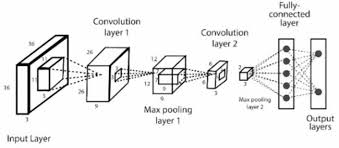
\includegraphics[scale=0.8]{bab2/yolo.jpeg}
  \caption{\emph{Layer} pada YOLO \cite{sohel2021music}}
  \label{fig:layeryolo}
\end{figure}

Pada Gambar \ref{fig:layeryolo} terlihat bahwa arsitektur CNN untuk pemrosesan citra. Proses dimulai dengan \emph{input layer} sebagai inputan gambar. Kemudian, \emph{convolution layer 1}, untuk ekstraksi fitur pada citra. Setelah itu, melewati \emph{max pooling layer 1} untuk mengurangi dimensi data dalam meningkatkan efisiensi program komputasi saat melakukan pemrosesan data sehingga mencegah \emph{overfitting}. Akan seterusnya mengulang \emph{layer} tersebut hingga pada tahap akhir, hasilnya berhasil menuju \emph{fullly-connected layer} yang mengkoneksikan semua neuron dengan tujuan menghasilkan keluaran di \emph{output layer} \cite{layercnn}.

Seiring berkembangnya kebutuhan akan deteksi objek yang lebih akurat dan efisien, berbagai varian YOLO telah diperkenalkan dengan peningkatan signifikan dalam arsitektur dan performa. Salah satu contohnya adalah YOLOv5, yang mengintegrasikan fitur-fitur seperti Cross Stage Partial Networks (CSPNet) untuk mengurangi redundansi dan meningkatkan efisiensi pemrosesan. Selain itu, YOLOv6 memperkenalkan EfficientRep Backbone dan Rep-PAN Neck, yang dirancang untuk meningkatkan ekstraksi dan agregasi fitur, sehingga menghasilkan deteksi objek yang lebih akurat dan cepat. Evaluasi pada dataset COCO menunjukkan bahwa YOLOv6-N mencapai 37,5\% AP dengan kecepatan 1187 FPS pada GPU NVIDIA Tesla T4, menjadikannya salah satu model deteksi objek real-time terdepan saat ini \cite{li2024yolov6}.

\subsection{YOLOv8}
YOLOv8 merupakan versi terkini dari \emph{framework} YOLO, yang dikembangkan untuk mendeteksi objek pada sebuah data seperti gambar dan video secara \emph{real-time} dengan kecepatan tinggi. YOLOv8 dirancang untuk menyelaraskan akurasi deteksi dan kecepatan pemrosesan sehingga cocok untuk berbagai implementasi aplikasi seperti pengawasan dan pemantauan keamanan, lalu lintas, dan pemantauan lainnya yang membutuhkan deteksi objek secara cepat dan akurat.

YOLOv8 menggabungkan beberapa pendekatan yang lebih baik, antara lain \emph{Feature Pyramid Network} (FPN) untuk mengatur objek yang bervariasi, kemudian ada \emph{Path Aggregation Network} (PAN) yang membuat kualitas deteksi pada beberapa level fitur meningkat. YOLOv8 sudah mampu mengurangi redudansi dari komputasi melalui pemisahan fitur dengan \emph{backbone} CSPDarknet sehingga hasil dari pemrosesan dapat lebih efisien. Selain itu, pendekatan \emph{anchor-free} dalam \emph{Adaptive Anchor-free Head} digunakan oleh YOLOv8 guna menghilangkan \emph{anchor-box} dan meningkatkan fleksibilitas. Maka dari itu, YOLOv8 memberikan performa deteksi objek yang lebih baik secara keseluruhan \cite{yolov8}.

Selain keunggulan teknisnya, YOLOv8 juga hadir dengan dukungan ekosistem yang lebih matang melalui integrasi dengan Ultralytics API dan format konfigurasi yang lebih sederhana, sehingga memudahkan peneliti maupun pengembang dalam pelatihan dan deployment model. Fitur-fitur baru seperti \emph{auto-learning rate finder}, visualisasi augmentasi, serta ekspor ke berbagai format seperti TensorRT, ONNX, dan CoreML memperluas fleksibilitas implementasinya pada berbagai perangkat \emph{edge} maupun \emph{cloud}. Hal ini menjadikan YOLOv8 sangat adaptif terhadap kebutuhan pengembangan sistem berbasis visi komputer di berbagai \emph{platform}, termasuk perangkat \emph{mobile}, sistem tertanam, dan server skala besar \cite{jocher2023ultralytics}.

\subsection{TensorRT}
Implementasi TensorRT pada model YOLOv8 bertujuan untuk mengoptimalkan proses inferensi dengan mengaplikasikan berbagai teknik percepatan seperti kuantisasi, \emph{layer fusion}, dan optimasi kernel yang dirancang khusus untuk perangkat keras NVIDIA GPU. TensorRT memproses model deep learning agar dapat dijalankan dengan latensi yang rendah dan throughput tinggi tanpa mengurangi akurasi, sehingga sangat sesuai untuk aplikasi \emph{real-time}. Dalam penelitian ini, TensorRT digunakan untuk meningkatkan kecepatan inferensi pada model YOLOv8 yang telah dimodifikasi pada arsitektur \emph{Feature Pyramid Network} (FPN), sehingga dapat memenuhi kebutuhan inferensi dengan latensi yang sangat singkat.

Hasil eksperimen menunjukkan bahwa implementasi TensorRT meningkatkan kecepatan inferensi secara signifikan, dengan penurunan waktu inferensi hingga 7,1 ms dibandingkan model tanpa optimasi. Peningkatan ini disertai dengan sedikit kenaikan nilai \emph{mean Average Precision} (mAP50-95), menandakan bahwa optimasi ini tetap menjaga akurasi deteksi objek. Modifikasi arsitektur YOLOv8 pada FPN yang hanya menggunakan detection head pada skala objek tertentu, dipadukan dengan TensorRT memberikan performa terbaik dalam hal kecepatan dan presisi. Pendekatan ini mempercepat inferensi hingga mencapai sekitar 12 ms, sangat ideal untuk implementasi dalam sistem deteksi berbasis visi komputer dengan kebutuhan respons waktu nyata \cite{tensorrt}.

Lebih lanjut, implementasi TensorRT tidak hanya meningkatkan kecepatan inferensi, tetapi juga memungkinkan efisiensi yang lebih tinggi dalam penggunaan sumber daya, khususnya pada perangkat edge dan embedded. Penelitian menunjukkan bahwa penggunaan TensorRT dalam \emph{deployment} jaringan deteksi objek pada perangkat \emph{edge} AI menghasilkan pengurangan waktu inferensi yang signifikan tanpa mengorbankan akurasi deteksi. Hal ini menegaskan bahwa optimasi \emph{runtime} menggunakan TensorRT sangat efektif untuk aplikasi \emph{real-time} yang dijalankan pada perangkat dengan keterbatasan sumber daya \cite{stacker2021deployment}.


\subsection{\emph{Observation-Centric} SORT (OC-SORT)}
Kalman Filter adalah salah satu metode utama yang sering digunakan dalam sistem pelacakan multi-objek, termasuk dalam algoritma \emph{SORT} (\emph{Simple Online and Realtime Tracking}). Metode ini berasumsi bahwa pergerakan objek mengikuti model gerak linear dengan kecepatan tetap pada rentang waktu yang singkat. Dalam pengaplikasiannya untuk pelacakan kendaraan menggunakan drone DJI Phantom 4 Pro dan metode YOLOv8 yang dijalankan pada Jetson Nano, Kalman Filter dipakai untuk memprediksi posisi kendaraan berdasarkan kotak pembatas (\emph{bounding box}) hasil deteksi objek. Namun, metode ini memiliki keterbatasan saat objek terhalang (\emph{occlusion}) atau bergerak dengan pola non-linear, sehingga akumulasi kesalahan prediksi dapat terjadi seiring berjalannya waktu.

OC-SORT (\emph{Observation-Centric SORT}) merupakan pengembangan dari \emph{SORT} yang mengatasi kelemahan tersebut dengan pendekatan yang berfokus pada observasi nyata, bukan hanya prediksi hasil estimasi. Metode ini mengadopsi strategi \emph{Observation-Centric Re-Update} (\emph{ORU}), di mana kesalahan yang menumpuk pada Kalman Filter selama periode \emph{occlusion} diperbaiki dengan menggunakan data observasi virtual yang dibentuk melalui interpolasi dari pengamatan terakhir sebelum \emph{occlusion} dan pengamatan saat objek kembali terlihat. Dengan pendekatan ini, \emph{OC-SORT} mampu meningkatkan akurasi pelacakan objek terutama saat kendaraan yang sempat terhalang muncul kembali, serta menambahkan komponen \emph{Observation-Centric Momentum} (\emph{OCM}) untuk memperbaiki pencocokan data berdasarkan arah dan kecepatan gerak yang diukur dari observasi historis\cite{Cao2023}.

Untuk lebih meningkatkan robust­itas pelacakan pada aliran video beresolusi tinggi, \emph{OC-SORT} kerap dipadukan dengan skema asosiasi dua tahap seperti \emph{ByteTrack}. Pada tahap pertama, deteksi berkualitas tinggi dipasangkan ke jalur aktif menggunakan biaya gabungan IoU dan \emph{OCM}; pada tahap kedua, deteksi bernilai rendah namun potensial dihubungkan guna memulihkan jalur yang hampir hilang. Integrasi ini mempertahankan jumlah \emph{ID-switch} seminimal mungkin tanpa menurunkan FPS pada Jetson Nano, karena seluruh kalkulasi tetap berada di ranah \emph{bounding box} tanpa menambah beban model \emph{embedding}. Evaluasi pada himpunan data \emph{VisDrone 2022} menunjukkan peningkatan HOTA sebesar 4{,}7 poin dibanding \emph{OC-SORT} murni \cite{Zhang2022ByteTrack}.

\subsection{ByteTrack}
ByteTrack adalah algoritma pelacakan \emph{Multi-Object Tracking} (MOT) yang meningkatkan akurasi dengan memanfaatkan hampir keseluruhan deteksi objek, dari deteksi dengan skor rendah dan deteksi dengan skor tinggi. Dengan metode ByteTrack, dapat mengatasi permasalahan deteksi objek yang tersembunyi dalam frame, serta fragmentasi jalur pelacakan yang sering terjadi pada objek yang tidak terdeteksi dalam frame berturut-turut. Keunggulan ByteTrack dalam pelacakan adalah melakukan asosiasi terhadap objek deteksi yang hilang dengan objek yang telah dilacak pada frame sebelumnya, dan juga ketika objek terhalang atau memiliki kualitas rendah. Sehingga, hal tersebut memungkinkan pemulihan objek yang hilang, serta meningkatkan kontinuitas pelacakan \cite{Zhang2022ByteTrack}.

\begin{figure} [H] \centering
  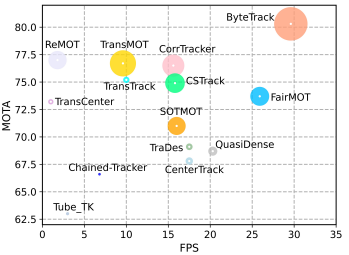
\includegraphics[scale=0.8]{bab2/mota_bytetrack.png}
  \caption{Perbandingan MOTA-IDFI-FPS terhadap \emph{tracker}}
  \label{fig:mota-tracker}
\end{figure}

Dalam grafik pada Gambar \ref{fig:mota-tracker} menunjukkan bahwa ByteTrack sebagai algoritma \emph{Multiple Object Tracking Accuracy} tertinggi dibandingkan dengan yang lain. ByteTrack sangat efisien dalam hal pelacakan sehingga FPS yang dihasilkan juga lebih tinggi meskipun tidak secepat FairMOT. Algoritma ByteTrack menggabungkan dua proses asosiasi dalam \emph{tracking} yang dilakukan. Pertama, deteksi pada skor tinggi (\emph{high-confidence}) yang memastikan pelacakan akurat pada objek yang tidak terhalang dan mencocokkan objek yang terdeteksi sebelumnya. Kedua, deteksi dengan skor rendah (\emph{low-confidence}), yang memungkinkan memulihkan objek yang sempat tidak terlacak dan terfragmentasi dalam frame sebelumnya. Penggunaan Kalman Filter dan algoritma Hungarian pada ByteTrack untuk mencocokkan deteksi baru dengan jalur \emph{tracking} yang telah ada sehingga memungkinkan \emph{tracking} yang lebih andal meskipun dalam kondisi berbeda-beda \cite{Zhang2022ByteTrack}.

\subsection{Ground Sampling Distance}
Ground Sampling Distance (GSD) adalah ukuran resolusi spasial citra udara yang menghubungkan satu piksel pada gambar dengan ukuran sebenarnya di permukaan tanah. Semakin kecil nilai GSD, semakin detail citra yang dihasilkan, karena setiap piksel mewakili area yang lebih kecil. Parameter ini krusial dalam fotogrametri dan aplikasi survei udara, karena akan menentukan sejauh mana objek di permukaan dapat dikenali dan diukur dengan akurat.

Secara matematis, GSD dapat dirumuskan sebagai berikut:
\begin{equation}
  \label{eq:gsd_basic}
  \mathrm{GSD}
  = \frac{H \times \mathrm{PixelSize}}{f}
\end{equation}
Di sini $H$ menyatakan ketinggian terbang (dalam meter), $f$ adalah panjang fokus kamera (dalam milimeter), dan \emph{PixelSize} adalah ukuran satu piksel pada sensor, yang dihitung dari lebar sensor $S_w$ (mm) dibagi jumlah piksel pada sumbu lebar gambar $\mathrm{ImgW}$:
\begin{equation}
  \label{eq:pixel_size}
  \mathrm{PixelSize}
  = \frac{S_w}{\mathrm{ImgW}}
\end{equation}
Dengan menggantikan \eqref{eq:pixel_size} ke dalam \eqref{eq:gsd_basic}, diperoleh:
\begin{equation}
  \label{eq:gsd_full}
  \mathrm{GSD}
  = \frac{H \times S_w}{f \times \mathrm{ImgW}}
\end{equation}

Sebagai contoh, untuk penerbangan pada ketinggian $H = 20\,$m dengan lebar sensor $S_w = 12{,}83\,$mm, fokus $f = 8{,}6\,$mm, dan lebar citra $\mathrm{ImgW} = 5472$ piksel, nilai GSD yang diperoleh adalah sekitar
\[
  \mathrm{GSD}
  = \frac{20 \times 12{,}83}{8{,}8 \times 640}
  \approx 4{,}66\ \mathrm{cm/piksel}.
\]
Angka ini menunjukkan bahwa satu piksel pada citra setara dengan area seluas kurang lebih $4{,}68\,$cm di permukaan.

Dalam praktiknya, perubahan ketinggian terbang akan memengaruhi GSD secara linier: peningkatan $H$ akan menaikkan nilai GSD, sehingga detail citra cenderung berkurang. Selain itu, pemilihan ukuran sensor dan resolusi gambar juga perlu disesuaikan dengan tujuan pemetaan. Misalnya, pada drone DJI Phantom 4 Pro, variasi ketinggian terbang antara 20-40 m dapat menghasilkan GSD antara 4-8 cm/piksel, sehingga operator dapat memilih kombinasi parameter yang optimal untuk keseimbangan antara cakupan area dan ketajaman detail objek \cite{Tilon2023}.

Kesalahan horizontal pada \emph{ortofoto} umumnya berada di kisaran dua hingga tiga kali nilai GSD, sedangkan kesalahan vertikal pada \emph{digital surface model} (DSM) berkisar tiga hingga lima kali GSD. Apabila GSD melebihi 10~cm/piksel, kesalahan vertikal meningkat tajam—terutama pada medan bergelombang karena densitas sampel permukaan tidak lagi cukup rapat untuk merekonstruksi relief mikro secara akurat. Oleh sebab itu, penentuan GSD sebaiknya didasarkan pada tolok ukur akurasi spasial yang dibutuhkan pada produk peta akhir, bukan semata-mata pada batas ketinggian terbang atau spesifikasi sensor.




\cleardoublepage
\chapter{METODOLOGI}
\label{sec:chap3_metodologi}

\section*{ }
Pada penelitian ini nantinya akan terdiri dari lima langkah utama yaitu :
\begin{figure}[H]
	\centering
	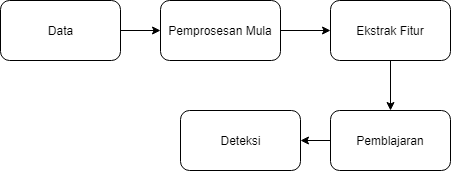
\includegraphics[width=\linewidth]{bab3/BlokDiagram}
	\caption{Blok Diagram Penelitian}
	\label{fig:blokdiagram}
\end{figure}


\section{Data}
Data adalah citra yang diperoleh dari kamera dengan ukuran $300\times 300$ dari beberapa sudut pandang yang berlainan.
\section{Pemprosesan Mula}
Citra yang telah diperoleh telah terpapar oleh gaussia noise sehingga perlu diperbaiki.
\section{Ekstraksi Fitur}
\lipsum[2]
\subsection{Fitur Warna}
\lipsum[1]
\subsection{Fitur Permukaan}
\section{Pembelajaran}
\lipsum[4]
\section{Deteksi}
\lipsum[2]







\cleardoublepage
\begin{spacing}{1.2}
	\chapter{PENGUJIAN, ANALISIS, DAN PERBANDINGAN}
	\label{sec:chap4_analisis}
\end{spacing}

\vspace{4ex}

Bab ini akan menunjukkan hasil pengujian dari sistem yang telah dibangun, kemudian dilakukan analisis terhadap hasil tersebut yang akan dijadikan bahan perbandingan dengan penelitian terdahulu. Dari hasil pengujian hingga kualitas sistem yang mana diperoleh perbedaan serta beberapa hal yang menjadi penyebab muncul perbedaan sistem antara penelitian ini dengan penelitian terdahulu.

\section{Alur Pengujian}
Alur pengujian beserta analisis perbandingan akan dijelaskan secara runtut sebagai berikut:

\begin{enumerate}[nolistsep]
    \item Pengujian model terhadap deteksi kendaraan
    \item Pengujian sistem dan perbandingan terhadap kecepatan rata-rata dibawah 25Km/H pada siang hari
    \item Pengujian sistem dan perbandingan terhadap kecepatan rata-rata diatas 25Km/H pada siang Hari
    \item Pengujian sistem terhadap kecepatan rata-rata 20Km/H pada malam hari
    \item Pengujian sistem terhadap kecepatan rata-rata 40Km/H pada malam hari
    \item Analisis terhadap kualitas sistem
\end{enumerate}

\section{Pengujian Model terhadap Deteksi Kendaraan}
Penelitian ini terdapat dua model yang telah dikembangkan, yaitu model deteksi kendaraan pada kondisi siang hari, dan kondisi malam hari.

\subsection{Model Deteksi Siang Hari}
Pelatihan model dengan kondisi siang hari yang menggunakan YOLOv8 dengan dilakukan epoch sebanyak 250 epochs, dengan setiap epoch memiliki \emph{value} yang berbeda-beda terhadap hasil akurasinya. Tabel akurasi hasil pelatihan model dapat dilihat pada Tabel \ref{table:akurasi model siang}.

\begin{table}[H]
	\caption{Akurasi Hasil Pelatihan Model pada Siang Hari}
    \label{table:akurasi model siang}
	\centering
	\begin{tabular}{|c|c|c|c|}
		\hline
		Epochs & Precision & Recall & mAP50 \\ \hline
		50 & 0.67893 & 0.68114 & 0.6863 \\ \hline
		100 & 0.76356 & 0.77383 & 0.72166  \\ \hline
		160 (\emph{best}) & 0.80555 & 0.79315 & 0.82471  \\ \hline
		200 & 0.79412 & 0.76758 & 0.77683 \\ \hline
		250 & 0.79412 & 0.76758 & 0.77683 \\ \hline
	\end{tabular}
\end{table}

Setelah dilakukan pelatihan didapatkan beberapa grafik yang menunjukkan tingkat akurasi dari model hasil pelatihan yang telah dibuat. Grafik hasil pelatihan model siang dapat dilihat pada Gambar \ref{fig:grafik model siang}.
\vspace{-3ex}
\begin{figure} [H] \centering
  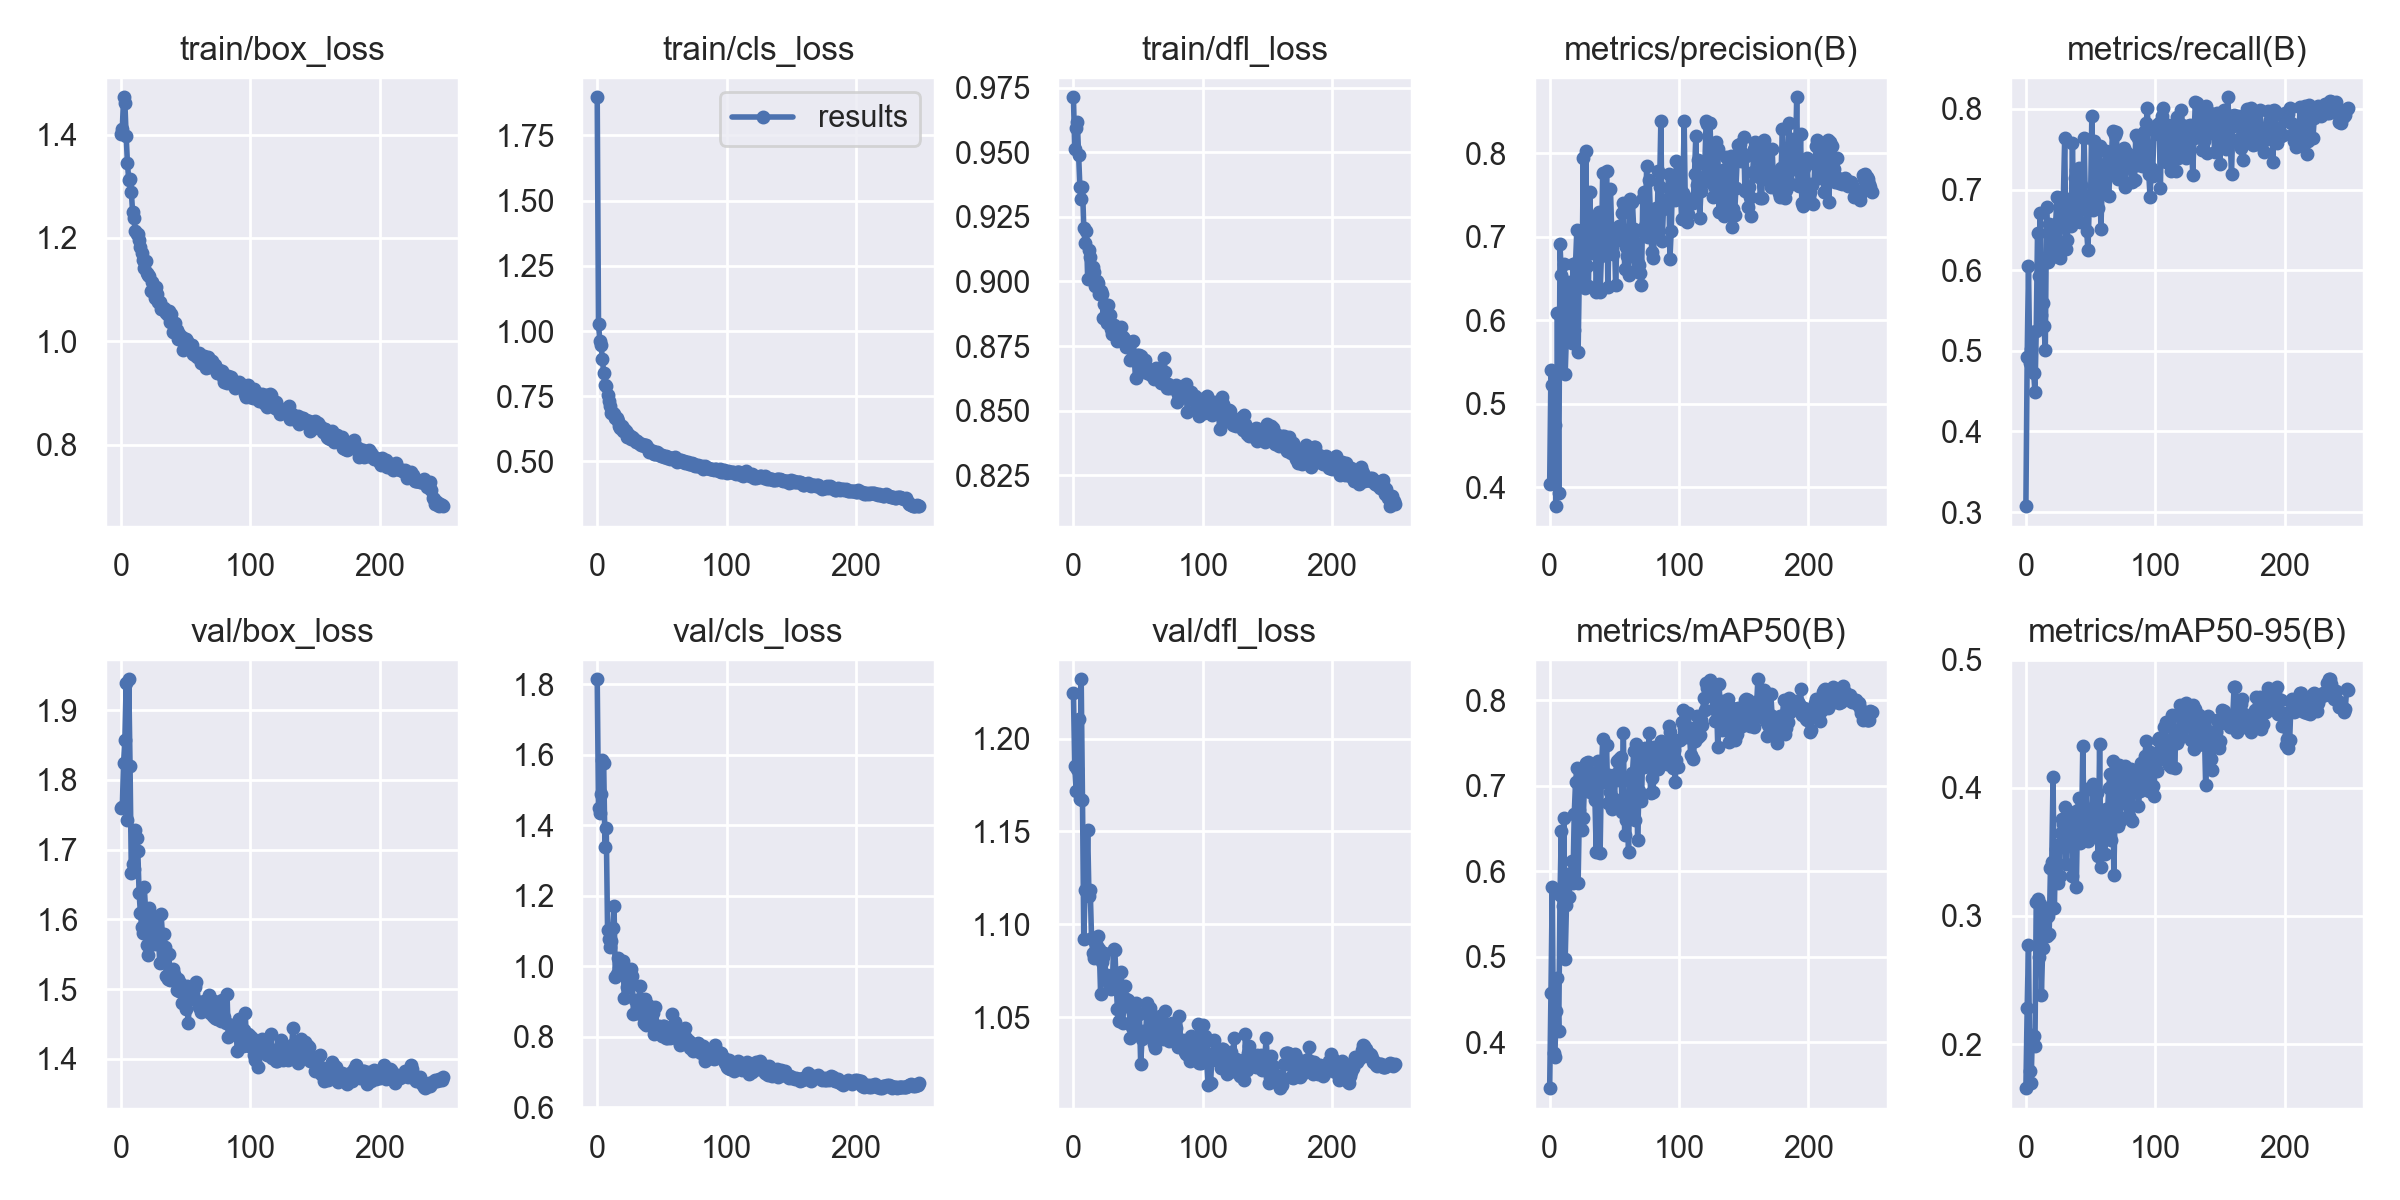
\includegraphics[scale=0.5]{bab4/results_siang.png}
  \caption{Grafik Hasil Pelatihan Model pada Siang Hari}
  \label{fig:grafik model siang}
\end{figure}
\vspace{-5ex}
Gambar \ref{fig:grafik model siang} menunjukkan kurva hasil pelatihan model YOLOv8 selama 250 epoch. Grafik \emph{train/box\_loss} dan \emph{val/box\_loss} menggambarkan penurunan \emph{bounding box loss} secara konsisten baik pada data pelatihan maupun validasi, yang mengindikasikan bahwa model semakin akurat dalam menentukan lokasi objek. Penurunan serupa juga terlihat pada \emph{train/cls\_loss} dan \emph{val/cls\_loss}, yang merefleksikan peningkatan kemampuan model dalam mengklasifikasikan objek dengan benar. Selain itu, distribusi nilai prediksi model terhadap \emph{ground truth} yang diukur melalui \emph{train/dfl\_loss} dan \emph{val/dfl\_loss} juga menunjukkan perbaikan yang stabil, menandakan bahwa prediksi model semakin mendekati nilai yang sebenarnya.

Grafik \emph{precision} dan \emph{recall} menunjukkan peningkatan yang signifikan seiring bertambahnya jumlah epoch, hingga mendekati nilai maksimum, yang berarti model semakin andal dalam mendeteksi objek secara akurat dan konsisten. Sementara itu, metrik mAP50 dan mAP50-95 juga memperlihatkan tren kenaikan yang stabil meskipun terdapat fluktuasi kecil, hal ini mencerminkan performa model yang semakin baik dalam berbagai tingkat ambang IoU. Secara keseluruhan, grafik-grafik pada Gambar \ref{fig:grafik model siang} memperlihatkan proses pelatihan yang berhasil, dengan peningkatan akurasi deteksi dan penurunan nilai loss yang menunjukkan bahwa model belajar secara efektif dari waktu ke waktu.

Dari hasil pelatihan model siang didapatkan juga confusion matrix yang dapat dilihat pada Gambar \ref{fig:confusion matrix siang}. \emph{Confusion matrix} yang dihasilkan merupakan fitur yang disediakan Ultralytics, sehingga dapat diketahui akurasi setiap \emph{class} yang dijadikan objek deteksi.

\begin{figure} [H] \centering
  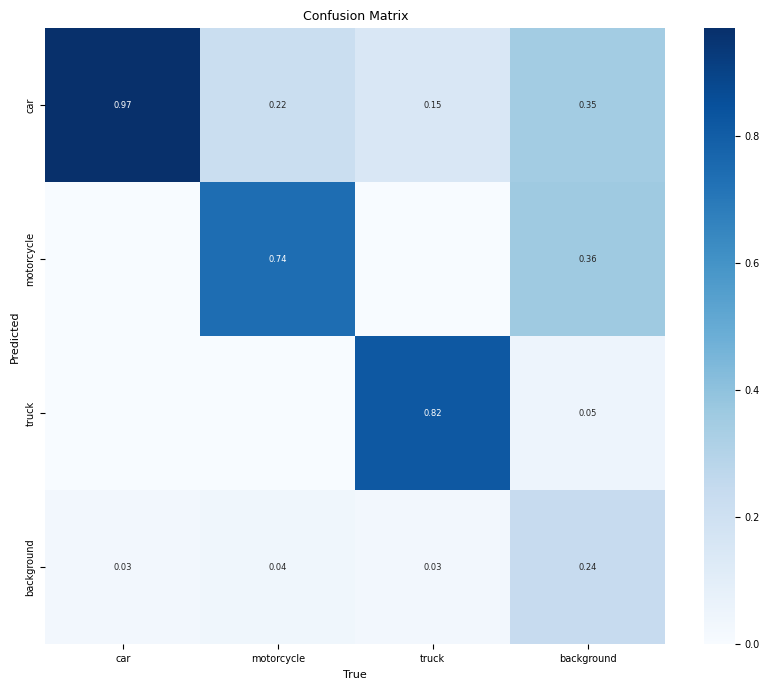
\includegraphics[scale=0.8]{bab4/confusion_siang.png}
  \caption{Confusion Matrix Model Siang Hari}
  \label{fig:confusion matrix siang}
\end{figure}
Pada Gambar \ref{fig:confusion matrix siang} menunjukkan confusion matrix dari hasil pelatihan model YOLOv8 pada kondisi siang hari. Setiap baris pada matriks ini merepresentasikan kelas yang diprediksi oleh model, sementara setiap kolom menunjukkan kelas sebenarnya dari objek yang terdeteksi. Matriks ini memberikan gambaran performa model dalam mengklasifikasikan empat kategori objek, yaitu \emph{car}, \emph{motorcycle}, \emph{truck}, dan \emph{background}.

\begin{enumerate}[nosep]
	\item Kelas \emph{car}:
	Model mengenali objek \emph{car} dengan cukup baik (97\% benar), dan sisanya kesalahan kecil mendteksi \emph{background}.

	\item Kelas \emph{motorcycle}:
	Sebanyak 74\% objek \emph{motorcycle} berhasil dikenali, tapi cukup banyak yang salah diprediksi sebagai \emph{car} (22\%).

	\item Kelas \emph{truck}:
	Akurasi pada kelas \emph{truck} juga tinggi (82\%), namun masih ada kesalahan kecil di \emph{background} sebesar 3\% dan \emph{car} (15\%).

	\item \emph{background}:
	Model tampak kesulitan membedakan latar, dengan 36\% \emph{motorcycle} dan 35\% diprediksi \emph{car}.
\end{enumerate}

Secara keseluruhan, model menunjukkan performa terbaik pada kelas \emph{car}, namun masih memerlukan perbaikan dalam mengidentifikasi objek \emph{motorcycle} dan \emph{background}, terutama untuk mengurangi tingkat kesalahan klasifikasi yang tinggi terhadap latar belakang.

Terdapat tahap validasi deteksi objek dari hasil pelatihan model siang yang telah dilakukan. Pada Gambar \ref{fig:validasi deteksi siang} dapat dilihat hasil deteksi dari model pelatihan beserta \emph{confidence threshold} yang diperoleh setiap objek deteksi.
\vspace{-3pt}
\begin{figure} [H] \centering
  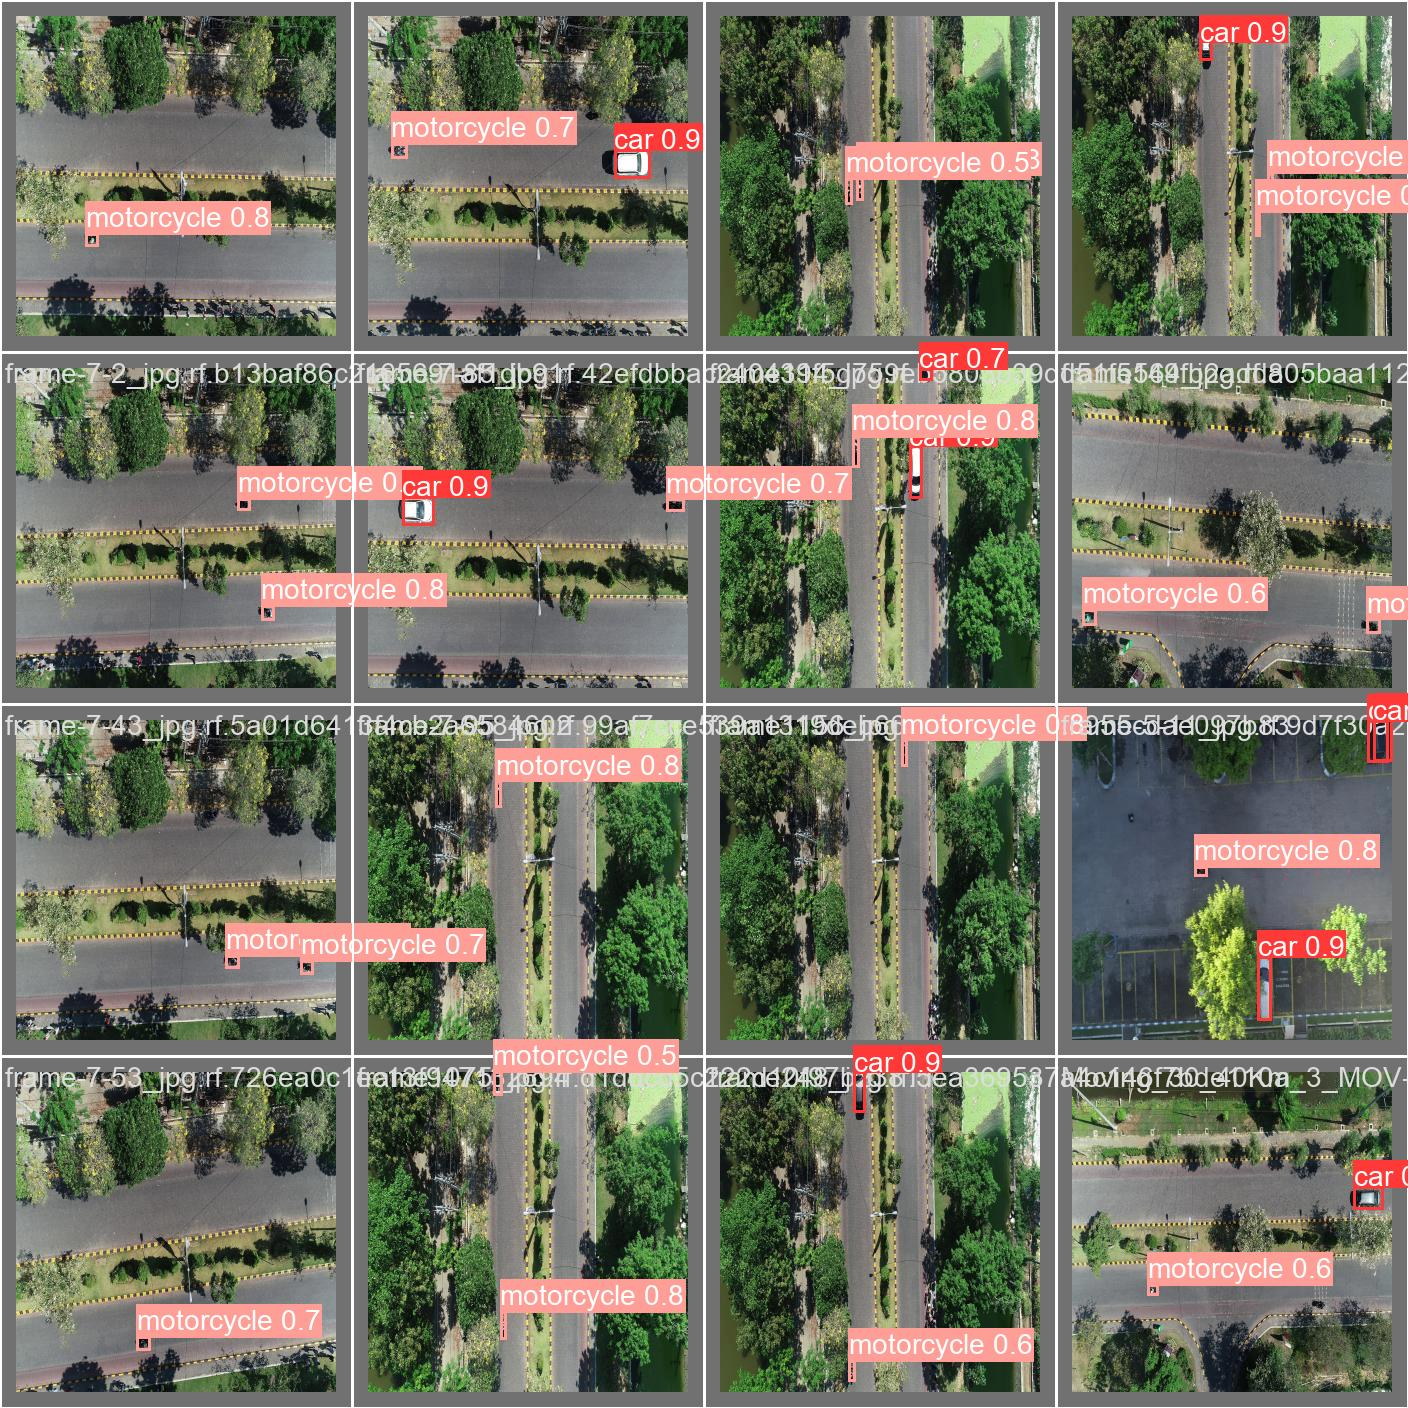
\includegraphics[scale=0.25]{bab4/val_batch_siang.jpg}
  \caption{Validasi Deteksi Siang Hari}
  \label{fig:validasi deteksi siang}
\end{figure}
\vspace{-3pt}
Dari hasil validasi didapatkan \emph{confidence threshold} untuk setiap objek terdeteksi diatas 0.5 dan ada dua objek motor terdeteksi yang mendapatkan 0.5.

\subsection{Model Deteksi Malam Hari}
Pelatihan model pada kondisi malam hari menggunakan YOLOv8 telah dilakukan selama 250 epoch, di mana setiap epoch menghasilkan \emph{value} akurasi yang bervariasi. Hasil akurasi dari proses pelatihan model tersebut disajikan pada Tabel \ref{table:akurasi model malam}.
\begin{table}[H]
	\caption{Akurasi Hasil Pelatihan Model pada Malam Hari}
    \label{table:akurasi model malam}
	\centering
	\begin{tabular}{|c|c|c|c|}
		\hline
		Epochs & Precision & Recall & mAP50 \\ \hline
		50 & 0.81247 & 0.8977 & 0.81938 \\ \hline
        72 (\emph{best}) & 0.94688 & 0.88395 & 0.92997 \\ \hline
		100 & 0.95264 & 0.88435 & 0.90664 \\ \hline
		200 & 0.9409 & 0.89202 & 0.906 \\ \hline
		250 & 0.92616 & 0.88637 & 0.88913 \\ \hline
	\end{tabular}
\end{table}

Dari hasil pelatihan model juga didapatkan grafik untuk setiap aspek yang diuji sehingga dapat dilihat apakah hasil model sudah sesuai yang diharapkan atau tidak. Grafik hasil pelatihan tersebut dapat dilihat pada Gambar \ref{fig:grafik model malam}. Hasil tersebut dapat digunakan sebagai acuan seberapa besar akurasi model hasil pelatihan yang telah dilakukan.

\begin{figure} [H] \centering
  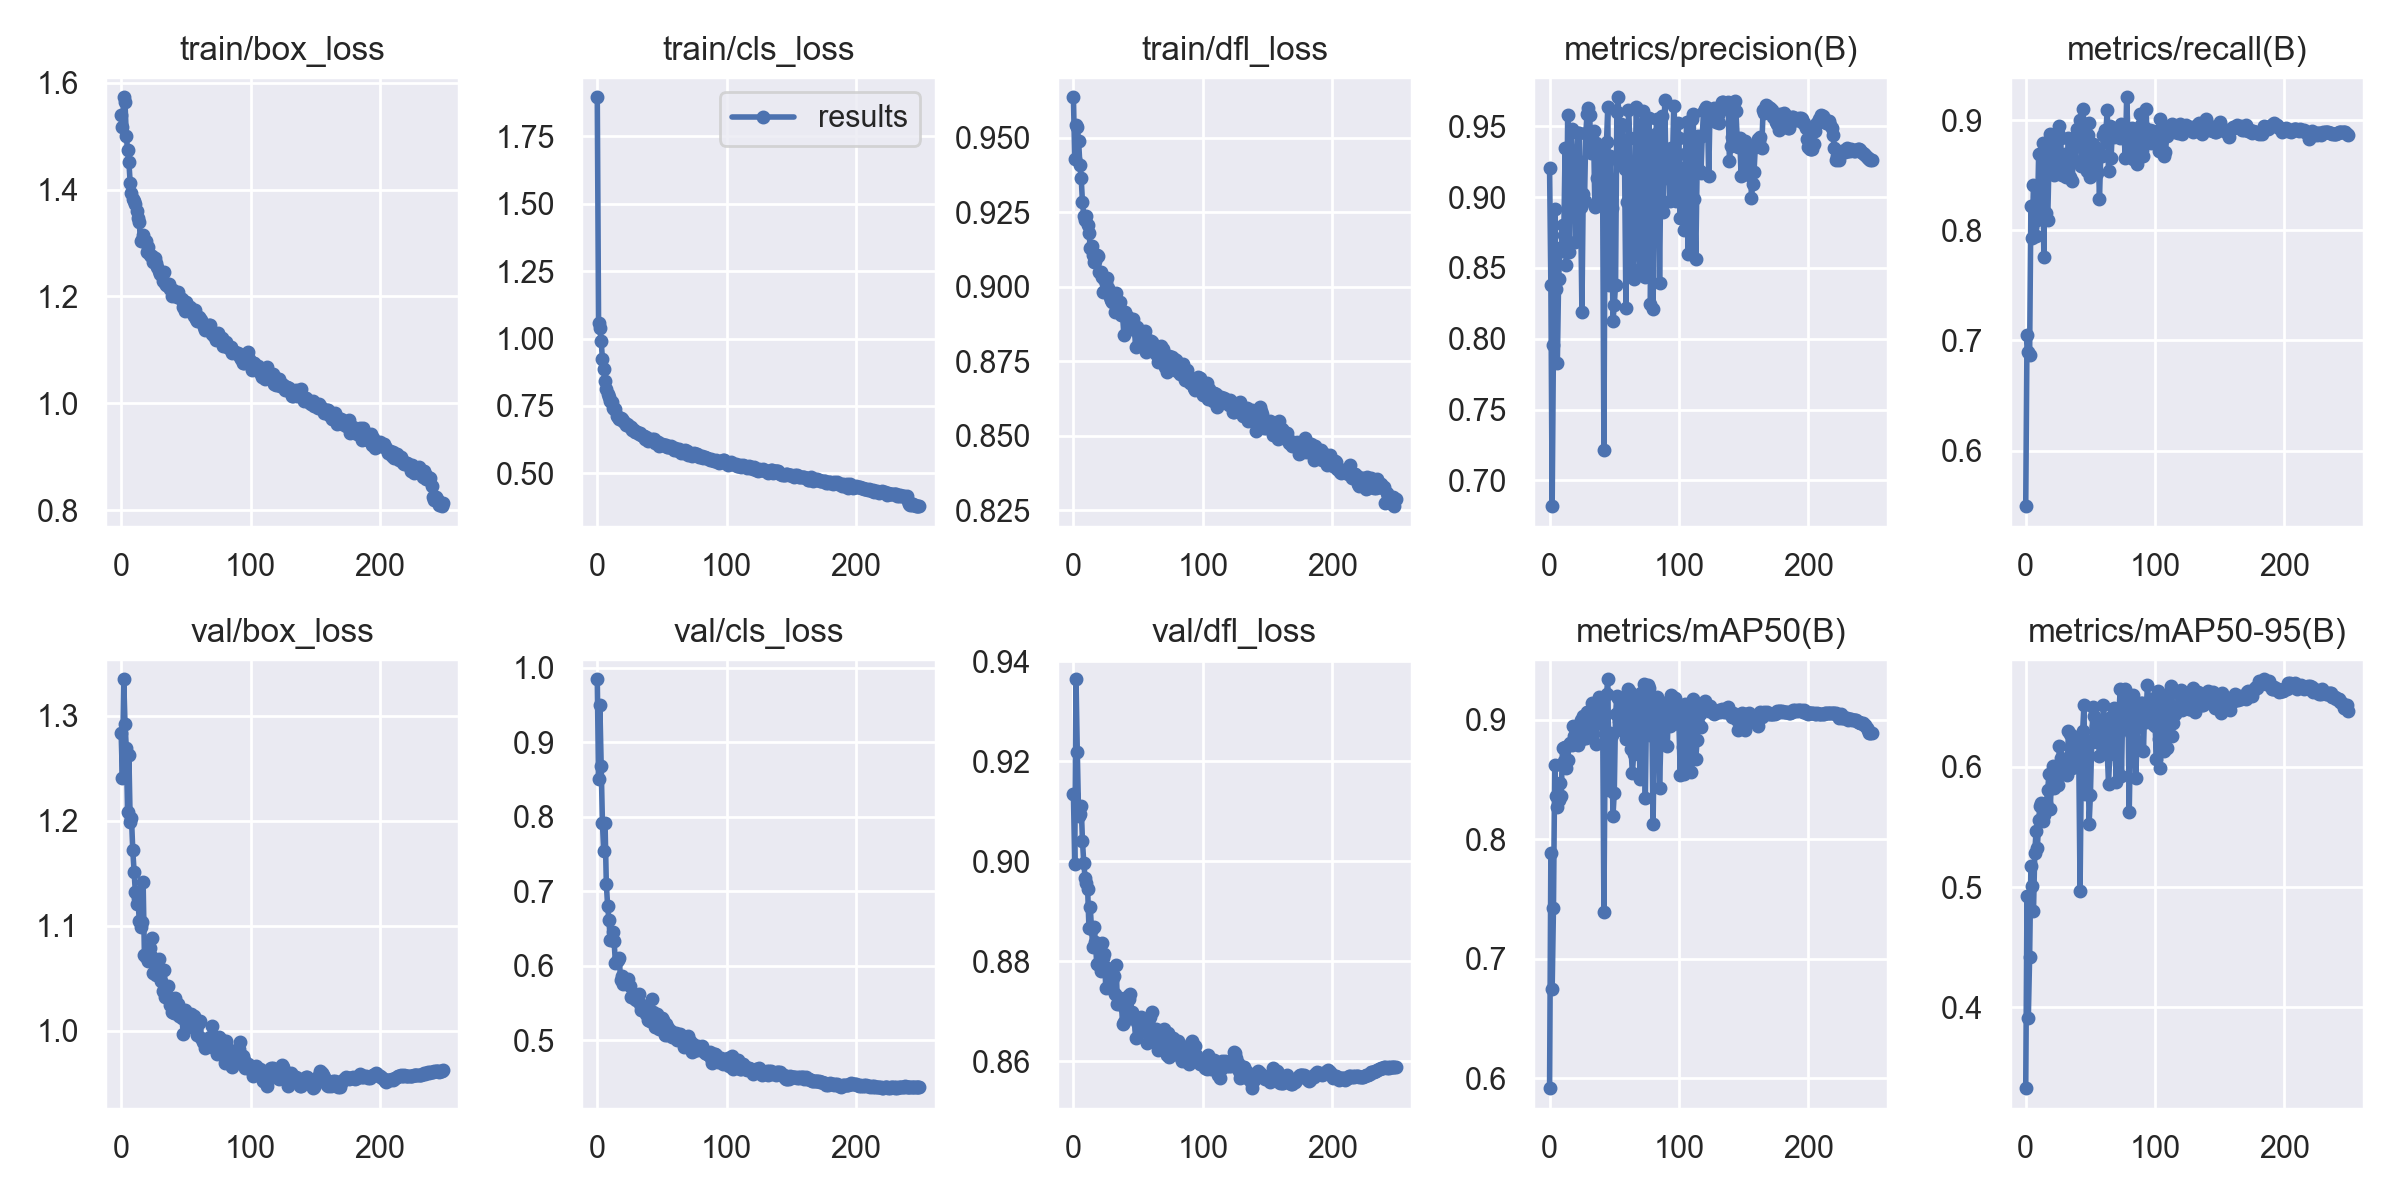
\includegraphics[scale=0.5]{bab4/grafik_model_malam.png}
  \caption{Grafik Hasil Pelatihan Model pada Malam Hari}
  \label{fig:grafik model malam}
\end{figure}

Gambar \ref{fig:grafik model malam} menunjukkan grafik-grafik hasil pelatihan model \emph{YOLOv8} yang dilatih selama 250 epoch. Grafik pertama, yaitu \emph{train/box\_loss} dan \emph{val/box\_loss}, menggambarkan \emph{bounding box loss} pada data pelatihan maupun data validasi. Kedua grafik ini menunjukkan penurunan yang stabil, yang menandakan bahwa model semakin baik dalam memprediksi posisi objek seiring dengan bertambahnya jumlah epoch. Demikian pula, grafik \emph{train/cls\_loss} dan \emph{val/cls\_loss} untuk \emph{classification loss} menunjukkan penurunan yang konsisten, menandakan bahwa model semakin akurat dalam mengklasifikasikan objek pada data pelatihan dan validasi. \emph{train/dfl\_loss} dan \emph{val/dfl\_loss} menunjukkan \emph{distribution for logits loss}, yang juga menurun dengan stabil, yang menunjukkan bahwa distribusi prediksi model semakin mendekati distribusi yang benar. Grafik \emph{metrics/precision} dan \emph{metrics/recall} menggambarkan \emph{precision} dan \emph{recall} model pada data pelatihan dan validasi. Seiring berjalannya epoch, kedua metrik ini menunjukkan peningkatan yang signifikan, dengan \emph{precision} dan \emph{recall} yang mendekati 1, menandakan bahwa model semakin efektif dalam mendeteksi objek dengan akurasi yang tinggi.

Di sisi lain, grafik \emph{metrics/mAP50} dan \emph{metrics/mAP50-95} menunjukkan \emph{mean Average Precision} (mAP) pada level IoU 0.5 dan rata-rata mAP pada interval 0.5 hingga 0.95. \emph{mAP50} menunjukkan performa deteksi model pada threshold IoU 0.5 dan terus meningkat, mencerminkan bahwa model semakin akurat dalam deteksi objek, sementara \emph{mAP50-95} menunjukkan performa model secara keseluruhan pada berbagai threshold IoU. Kedua grafik ini menunjukkan peningkatan yang stabil, meskipun terdapat sedikit fluktuasi, yang mungkin disebabkan oleh variasi dalam data validasi. Secara keseluruhan, grafik-grafik ini menunjukkan bahwa model \emph{YOLOv8} berhasil dilatih dengan baik, dengan peningkatan akurasi deteksi objek dan kemampuan model dalam mengurangi kerugian secara bertahap sepanjang 250 epoch pelatihan.

Kemudian terdapat hasil confusion matrix yang didapatkan dari hasil model pelatihan ini. Confusion matrix tersebut dapat dilihat pada Gambar .

\begin{figure} [H] \centering
  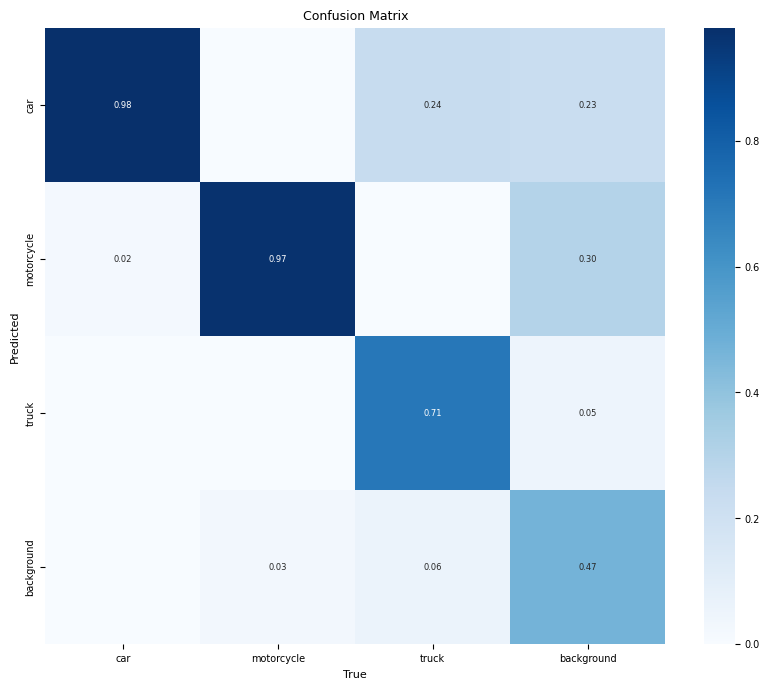
\includegraphics[scale=0.8]{bab4/confusion_malam.png}
  \caption{Confusion Matrix Model Malam Hari}
  \label{fig:confusion matrix malam}
\end{figure}
\vspace{-10pt}
Confusion matrix pada Gambar \ref{fig:confusion matrix malam} menunjukkan hasil prediksi model pada malam hari berdasarkan kategori objek yang terdeteksi.

\begin{enumerate}[nosep]
\item Kelas \emph{car}:
Model mampu mengenali objek \emph{car} dengan sangat baik, dengan tingkat keberhasilan 98\%. Meski demikian, masih ada 2\% yang keliru diklasifikasikan sebagai \emph{motorcycle}.

\item Kelas \emph{motorcycle}:  
Objek \emph{motorcycle} terdeteksi dengan akurasi 97\%, dan salah memprediksi sebagai \emph{background} sebesar 3\%.

\item Kelas \emph{truck}:  
Model berhasil mengenali 71\% objek \emph{truck} dengan benar. Terdapat salah prediksi sedikit dimana \emph{car} terprediksi sebanyak 24\%.

\item \emph{background}:  
Model mengenali \emph{background} hanya 47\%, sisanya menyebar di \emph{class} lain.
\end{enumerate}

Melalui analisis ini, dapat disimpulkan bahwa model \textit{YOLOv8} menunjukkan akurasi yang sangat baik dalam mendeteksi kelas \textit{car} dengan tingkat \textit{True Positive} yang sangat tinggi, sedangkan ada sedikit kesulitan dalam mendeteksi objek \textit{background} dan \textit{truck}.

Kemudian, dilakukan validasi deteksi objek dari hasil pelatihan model ini. Pada Gambar \ref{fig:validasi deteksi malam} dapat dilihat hasil model yang telah dilatih beserta \emph{confidence threshold} yang didapatkan untuk setiap citra yang digunakan sebagai validasi.

\begin{figure} [H] \centering
  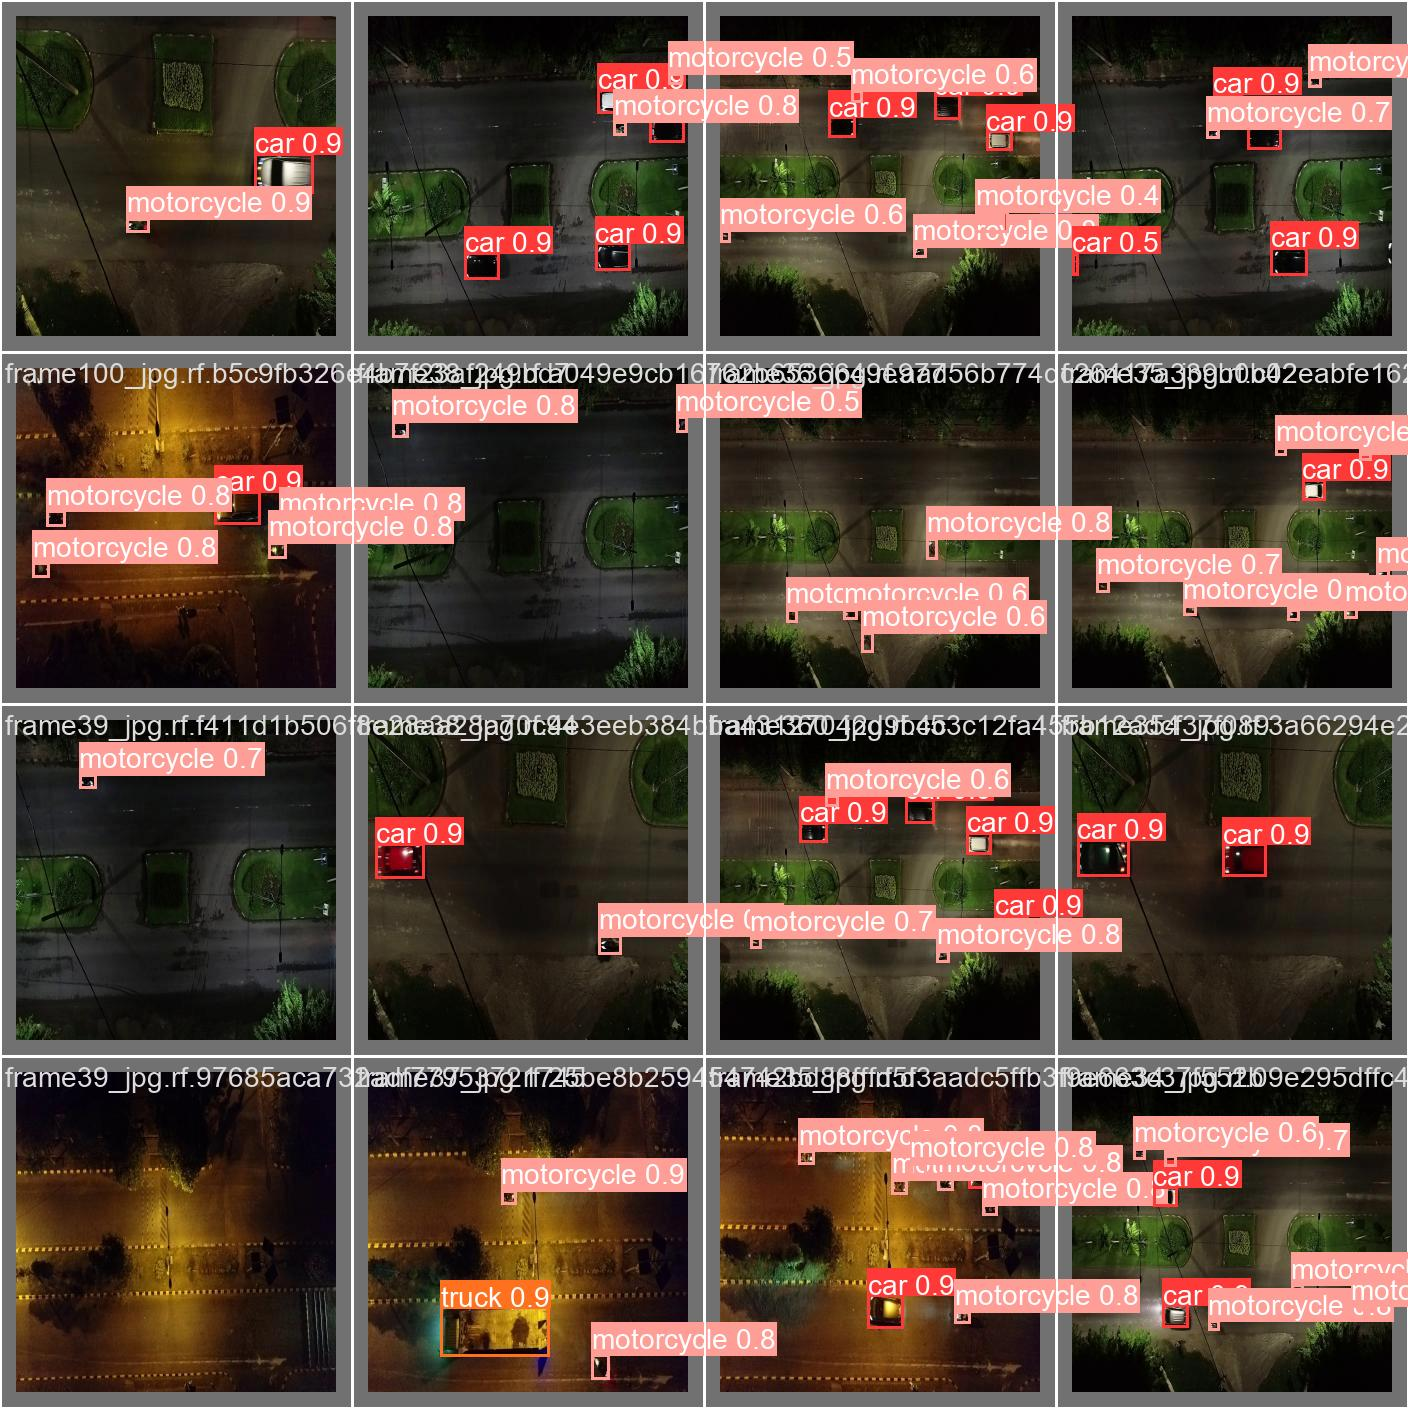
\includegraphics[scale=0.25]{bab4/val_batch_malam.jpg}
  \caption{Validasi Deteksi Malam Hari}
  \label{fig:validasi deteksi malam}
\end{figure}
\vspace{-10pt}
Dari hasil validasi deteksi tersebut objek kecil seperti motor mendapatkan nilai \emph{confidence threshold} paling kecil 0.5 dan paling tinggi 0.9. Untuk mobil rata-rata mendapatkan 0.8 hingga 0.9.

\section{Pengujian dan Perbandingan Sistem terhadap Kecepatan Rata-rata dibawah 25Km/H pada Siang Hari}
Dilakukan analisis terhadap pengujian yang didapatkan dari penelitian ini dan dilakukan perbandingan dengan penelitian terdahulu. Terdapat dua penelitian terdahulu yang digunakan, antara lain:
\begin{enumerate}[nolistsep]
  \item Perhitungan Kecepatan Kendaraan Menggunakan Drone Bergerak dengan Metode Deep Learning (Fatchurozi, 2024) \\
  \item Vehicle Tracking and Speed Estimation from Unmanned Aerial Vehicles Using Segmentation Initialised Trackers (Tilon \& Nex, 2023) \\
\end{enumerate}
\vspace{-5pt}
Pengujian ini dilakukan dengan kendaraan motor yang dikendarai dengan kecepatan rata-rata 20km/h dengan \emph{drone} diam. Tujuan dilakukan pengujian ini untuk mendapatkan informasi terkait kinerja terhadap sistem sejauh mana akurasi perhitungannya. Pengujian dilakukan pada siang hari dengan \emph{interval} waktu antara 11.00 WIB hingga 13.00 WIB. Referensi untuk hasil sistem digunakan perhitungan manual di setiap ketinggian. 

\begin{table}[H]
	\caption{Perhitungan Manual dengan Kecepatan Rata-rata 20km/h pada Siang Hari}
    \label{table:20km/h-siang-manual}
	\centering
	\begin{tabular}{|c|c|c|c|c|}
		\hline
		\multirow{2}{*}{\textbf{Ketinggian (Meter)}} & \multicolumn{3}{c|}{\textbf{Rata-rata Kecepatan (Km/h)}} & \multirow{2}{*}{\textbf{Rata-rata (Km/h)}} \\ \cline{2-4}
		& 1 & 2 & 3 & \\ \hline
		20 & 23,33 & 22,9 & 22,3 & 22,84 \\
		30 & 18,94 & 18,8 & 18,76 & 18,83 \\
		40 & 18,81 & 18,79 & 18,72 & 18,77 \\ \hline
	\end{tabular}
\end{table}
\vspace{-10pt}
\begin{table}[H]
	\caption{Perhitungan Manual Penelitian \ref{subsec:Iqbal2024} dengan Kecepatan Rata-rata 20km/h pada Siang Hari}
    \label{table:20km/h-siang-manual-iqbal}
	\centering
	\begin{tabular}{|c|c|c|c|c|}
		\hline
		\multirow{2}{*}{\textbf{Ketinggian (Meter)}} & \multicolumn{3}{c|}{\textbf{Rata-rata Kecepatan (Km/h)}} & \multirow{2}{*}{\textbf{Rata-rata (Km/h)}} \\ \cline{2-4}
		& 1 & 2 & 3 & \\ \hline
		20 & 19,46 & 19,71 & 19,86 & 19,67 \\
		30 & 19,31 & 18,77 & 18,93 & 19,00 \\
		40 & 19,48 & 18,81 & 18,87 & 19,05 \\ \hline
	\end{tabular}
\end{table}
\vspace{-10pt}
\begin{table}[H]
	\caption{Perhitungan Manual Penelitian \ref{subsec:Tilon2023} dengan Kecepatan Rata-rata 15 km/h}
    \label{table:15kmh-manual-Tilon}
	\centering
	\begin{tabular}{|c|c|}
		\hline
		\textbf{Ketinggian (Meter)} & \textbf{Kecepatan Aktual(Km/h)}\\ \hline
		50 & 14,68 \\ \hline
	\end{tabular}
\end{table}

Pada Tabel \ref{table:20km/h-siang-manual} yang menunjukkan hasil perhitungan manual dari penelitian ini dengan Tabel \ref{table:20km/h-siang-manual-iqbal} terdapat perbedaan di setiap ketinggiannya terutama pada ketinggian 20 meter yang memiliki selisih hingga 3km/h. Hal ini dapat disebabkan karena beberapa faktor \emph{error} yang dilakukan peneliti baik dalam mengukur jarak aktual dan waktu aktual saat objek yang menjadi objek percobaan melintas. Untuk Penelitian \ref{subsec:Tilon2023} yang ditunjukkan pada Tabel \ref{table:15kmh-manual-Tilon} memiliki kecepatan aktual yang tidak jauh dari target kecepatannya 15km/h.

Kemudian, dilakukan pengujian sistem dengan diberikan informasi tambahan, antara lain standar deviasi, dan \emph{error} antara hasil pengujian dengan perhitungan manual. Standar deviasi digunakan untuk mengetahui seberapa jauh hasil rata-rata dengan setiap data sehingga didapatkan informasi apakah tiap titik data bervariasi sangat jauh atau tidak untuk perbedaannya. Dapat dilihat pada Persamaan \ref{eq:standardeviasi} yang akan digunakan untuk menghitung standar deviasi:

\begin{equation}
\sigma = \sqrt{\frac{\sum_{i=1}^n (x_i - \mu)^2}{n}} \label{eq:standardeviasi}
\end{equation}

Dimana:

\[
\begin{aligned}
\sigma & = \text{Standar Deviasi} \\
n & = \text{Jumlah data} \\
x_i & = \text{Data ke-i} \\
\mu & = \text{Rata-rata}
\end{aligned}
\]

Kemudian, untuk menghitung \emph{error} setiap data digunakan persamaan \ref{eq:error}, \ref{eq:absolute_error}, \ref{eq:relative_error}:

\begin{equation}
\text{Error} = \text{Hasil Pengujian Sistem} - \text{Hasil Perhitungan Manual} \label{eq:error}
\end{equation}

\begin{equation}
\text{Absolute Error} = \left| \text{Error} \right| \label{eq:absolute_error}
\end{equation}

\begin{equation}
\text{Relative Error} = \left( \frac{\text{Absolute Error}}{\text{Hasil Perhitungan Manual}} \right) \times 100\% \label{eq:relative_error}
\end{equation}

Persamaan perhitungan akurasi dapat dilihat pada Persamaan \ref{eq:accuracy}:

\begin{equation}
\text{Accuracy} = 100\% - \text{Relative Error} \label{eq:accuracy}
\end{equation}

Pengujian di beberapa titik dengan kecepatan rata-rata 20km/h untuk ketinggian 20m, 30m, dan 40m, dapat dilihat pada Gambar \ref{fig:uji20m_20kmh} 

\begin{figure}[H]
  \centering
  \begin{subfigure}[b]{0.45\textwidth}
    \centering
    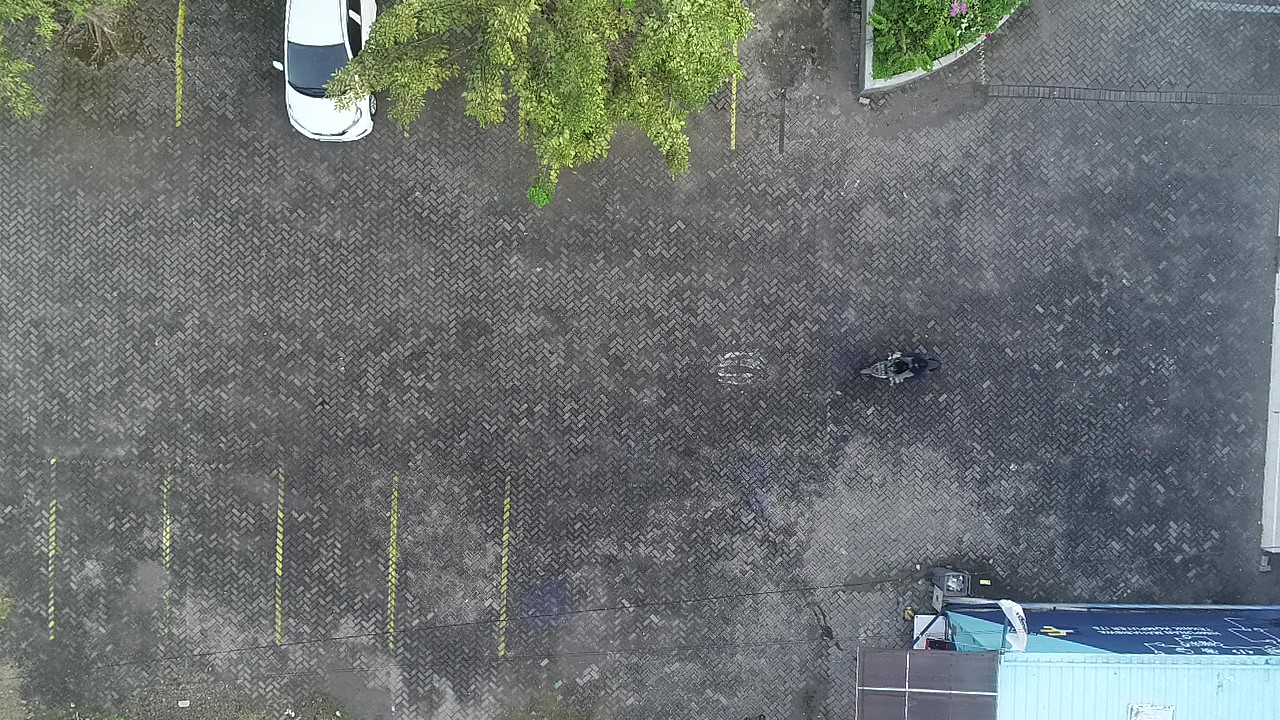
\includegraphics[width=\linewidth]{bab4/20m_siang_20km.jpg}
    \caption{Ketinggian 20 Meter}
    \label{fig:20m_siang_20kmh}
  \end{subfigure}%
  \hfill
  \begin{subfigure}[b]{0.45\textwidth}
    \centering
    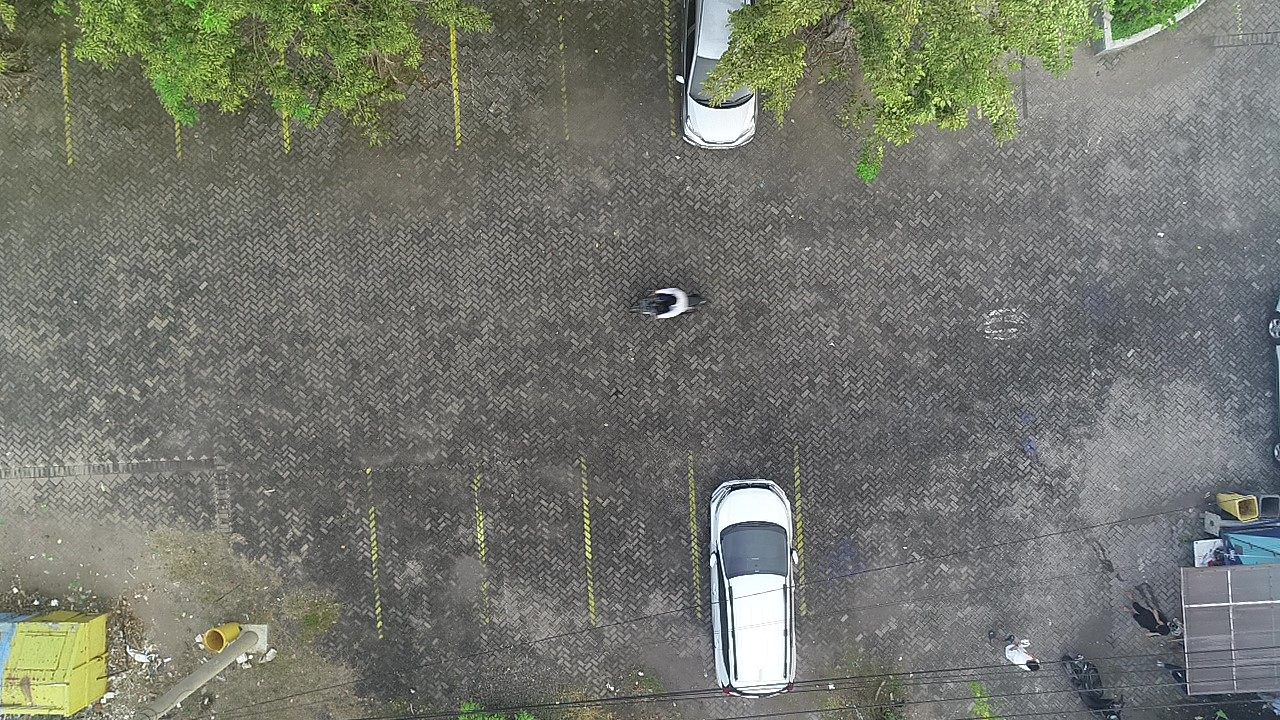
\includegraphics[width=\linewidth]{bab4/30m_siang_20km.jpg}
    \caption{Ketinggian 30 Meter}
    \label{fig:30m_siang_20kmh}
  \end{subfigure}%
  \hfill
  \begin{subfigure}[b]{0.45\textwidth}
    \centering
    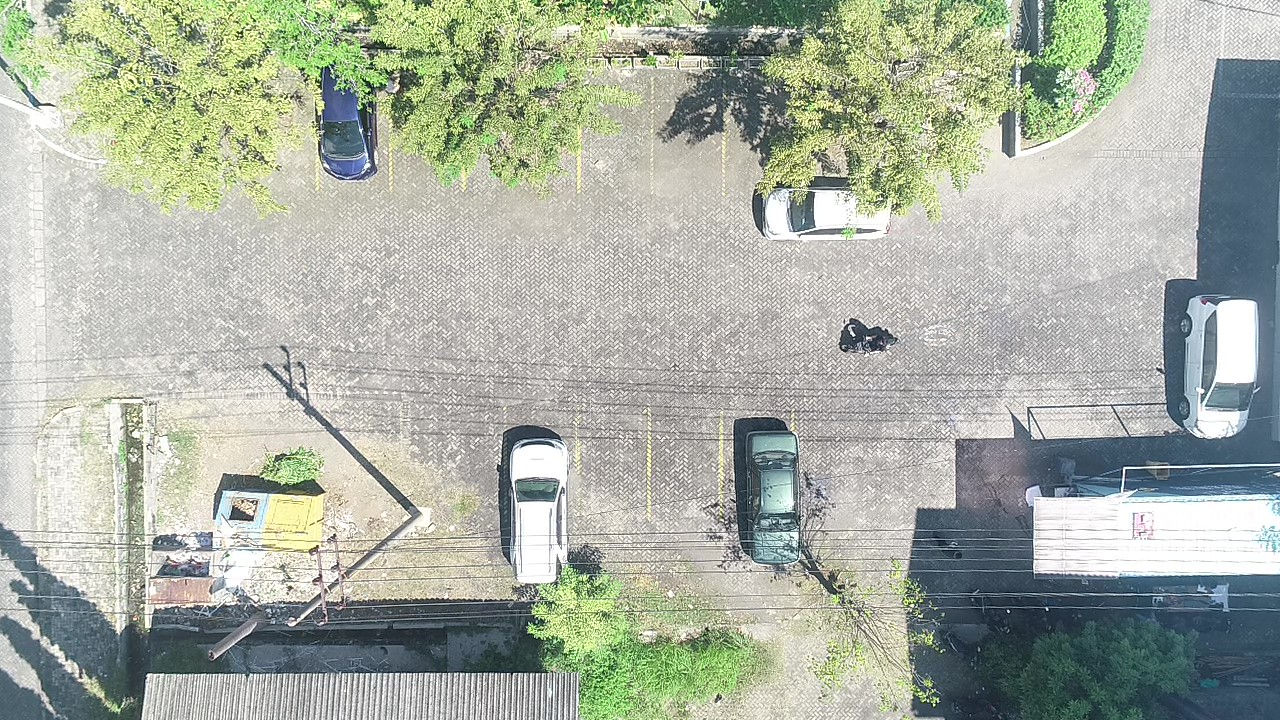
\includegraphics[width=\linewidth]{bab4/40m_siang_20km.jpg}
    \caption{Ketinggian 40 Meter}
    \label{fig:40m_siang_20kmh}
  \end{subfigure}
  \caption{Pengujian Sistem dengan Kecepatan Rata-rata 20km/h pada Siang Hari}
  \label{fig:uji20m_20kmh}
\end{figure}

Berikut data hasil pengujian yang telah dilakukan beserta hasil dari penelitian terdahulu dapat dilihat pada Tabel \ref{table:20km/h-siang-sistem}, Tabel \ref{table:20km/h-siang-iqbal}, dan Tabel \ref{table:15kmh-sistem-Tilon}.

\begin{table}[H]
	\caption{Pengujian dengan Kecepatan Rata-rata 20km/h pada Siang Hari}
    \label{table:20km/h-siang-sistem}
	\centering
	\begin{tabular}{|c|c|c|c|c|c|}
		\hline
		\multirow{2}{*}{\makecell{\textbf{Ketinggian} \\ \textbf{(Meter)}}}& \multicolumn{3}{c|}{\textbf{Rata-rata Kecepatan (Km/h)}} & \multirow{2}{*}{\makecell{\textbf{Rata-rata} \\ \textbf{(Km/h)}}} & \multirow{2}{*}{\makecell{\textbf{Standar} \\ \textbf{Deviasi}}} \\ \cline{2-4}
		& 1 & 2 & 3 & \\ \hline
		20 & 21,59 & 20,06 & 21,61 & 21,09 & 0,72\\
		30 & 23,28 & 21,25 & 25,05 & 23,19 & 1,55\\
		40 & 22,24 & 24,39 & 21,7 & 22,78 & 1,16\\ \hline
	\end{tabular}
\end{table}
\vspace{-10pt}
\begin{table}[H]
	\caption{Pengujian Peneletian \ref{subsec:Iqbal2024} dengan Kecepatan Rata-rata 20km/h pada Siang Hari}
    \label{table:20km/h-siang-iqbal}
	\centering
	\begin{tabular}{|c|c|c|c|c|c|}
		\hline
		\multirow{2}{*}{\makecell{\textbf{Ketinggian} \\ \textbf{(Meter)}}} & \multicolumn{3}{c|}{\textbf{Rata-rata Kecepatan (Km/h)}} & \multirow{2}{*}{\makecell{\textbf{Rata-rata} \\ \textbf{(Km/h)}}} & \multirow{2}{*}{\makecell{\textbf{Standar} \\ \textbf{Deviasi}}} \\ \cline{2-4}
		& 1 & 2 & 3 & \\ \hline
		20 & 17,86 & 18,64 & 18,62 & 18,37 & 1,61 \\ 
		30 & 17,80 & 17,84 & 17,64 & 17,76 & 0,97 \\ 
		40 & 17,69 & 17,90 & 17,90 & 17,83 & 1,10 \\ \hline
	\end{tabular}
\end{table}
\vspace{-10pt}
\begin{table}[H]
	\caption{Pengujian Penelitian \ref{subsec:Tilon2023} dengan Kecepatan Rata-rata 15 km/h}
    \label{table:15kmh-sistem-Tilon}
	\centering
	\begin{tabular}{|c|c|}
		\hline
		\textbf{Ketinggian (Meter)} & \textbf{Kecepatan Prediksi(Km/h)} \\ \hline
		50 & 17,97 \\ \hline
	\end{tabular}
\end{table}

Hasil pengujian menunjukkan rata-rata kecepatan kendaraan antara 21,09 hingga 23,19 km/h dengan variasi terbesar pada ketinggian 30 meter. Jika dibandingkan dengan perhitungan manual yang juga menggunakan target kecepatan 20 km/h, rata-rata kecepatan manual berada di kisaran 18,77 hingga 22,84 km/h, sehingga dapat diketahui terdapat selisih antara perhitungan manual dan sistem. Dibandingkan dengan penelitian 2.1.1 yang juga menargetkan kecepatan 20 km/h, hasilnya lebih rendah, yakni sekitar 17-18 km/h dan apabila melihat perhitungan manual yang memiliki rata-rata kecepatan sekitar 19 km/h, terdapat selisih antara perhitungan manual dan sistem dengan variasi yang lebih kecil. Sementara itu, penelitian 2.1.2 yang menargetkan kecepatan 15 km/h pada ketinggian 50 meter mencatat kecepatan aktual 14,68 km/h dan prediksi 17,97 km/h, yang sedikit lebih tinggi dari target.

Setelah didapatkan hasil pengujian maka akan dicari seberapa akurat sistem melalui perhitungan \emph{error}.

\begin{table}[H]
\centering
\caption{Perhitungan Error dan Akurasi dengan Kecepatan Rata-rata 20Km/h saat Siang Hari pada Percobaan 1}
\label{table:error_accuracy_titik1}
\begin{tabular}{|c|c|c|c|c|}
\hline
\textbf{Ketinggian (m)} & \textbf{Error} & \textbf{Absolute Error} & \textbf{Relative Error (\%)} & \textbf{Accuracy (\%)} \\ \hline
20 & -1.74 & 1.74 & 7.46 & 92.54 \\
30 & 4.34 & 4.34 & 22.91 & 77.09 \\
40 & 3.43 & 3.43 & 18.23 & 81.77 \\ \hline
\end{tabular}
\end{table}
\vspace{-3ex}
\begin{table}[H]
\centering
\caption{Perhitungan Error dan Akurasi Kecepatan Rata-rata 20Km/h saat Siang Hari pada Percobaan 2}
\label{table:error_accuracy_titik2}
\begin{tabular}{|c|c|c|c|c|}
\hline
\textbf{Ketinggian (m)} & \textbf{Error} & \textbf{Absolute Error} & \textbf{Relative Error (\%)} & \textbf{Accuracy (\%)} \\ \hline
20 & -2.84 & 2.84 & 12.41 & 87.59 \\
30 & 2.45 & 2.45 & 13.03 & 86.97 \\
40 & 5.60 & 5.60 & 29.79 & 70.21 \\ \hline
\end{tabular}
\end{table}
\vspace{-3ex}
\begin{table}[H]
\centering
\caption{Perhitungan Error dan Akurasi Kecepatan Rata-rata 20Km/h saat Siang Hari pada Percobaan 3}
\label{table:error_accuracy_titik3}
\begin{tabular}{|c|c|c|c|c|}
\hline
\textbf{Ketinggian (m)} & \textbf{Error} & \textbf{Absolute Error} & \textbf{Relative Error (\%)} & \textbf{Accuracy (\%)} \\ \hline
20 & -0.69 & 0.69 & 3.10 & 96.90 \\
30 & 6.29 & 6.29 & 33.55 & 66.45 \\
40 & 2.98 & 2.98 & 15.91 & 84.09 \\ \hline
\end{tabular}
\end{table}
Tabel hasil perhitungan \emph{error} dari pengujian menunjukkan akurasi pengukuran kecepatan \emph{drone} pada tiga percobaan dan ketinggian berbeda. Percobaan 1 memiliki akurasi tertinggi 92,54\% di 20 m, turun ke 77,09\% di 30 m, lalu naik ke 81,77\% di 40 m. Percobaan 2 akurasinya terbaik 87,59\% di 20 m dan terendah 70,21\% di 40 m. Percobaan 3 mencatat akurasi tertinggi 96,90\% di 20 m dan terendah 66,45\% di 30 m. Secara keseluruhan, ketinggian 20 meter cenderung memberikan hasil pengukuran paling akurat dan konsisten.

\begin{table}[H]
\centering
\caption{Akurasi pada Penelitian \ref{subsec:Iqbal2024} dengan Kecepatan Rata-rata 20 km/h saat Siang Hari}
\label{table:accuracy_iqbal}
\begin{tabular}{|c|c|c|c|}
\hline
\textbf{Ketinggian (m)} & \textbf{Percobaan 1 (\%)} & \textbf{Percobaan 2 (\%)} & \textbf{Percobaan 3 (\%)} \\ \hline
20 & 89.75 & 90.52 & 88.26 \\
30 & 93.47 & 91.55 & 87.98 \\
40 & 86.11 & 94.96 & 89.13 \\ \hline
\end{tabular}
\end{table}

\begin{table}[H]
\centering
\caption{Akurasi pada Penelitian \ref{subsec:Tilon2023} dengan Kecepatan Rata-rata 15 km/h}
\label{table:accuracy_tilon}
\begin{tabular}{|c|c|}
\hline
\textbf{Ketinggian (m)} & \textbf{Percobaan 1 (\%)} \\ \hline
50 & 77,59 \\ \hline
\end{tabular}
\end{table}

Berdasarkan hasil pengujian yang dilakukan beserta perbandingan dengan data penelitian terdahulu, beberapa hal yang dapat disimpulkan terkait akurasi pengukuran kecepatan kendaraan menggunakan drone adalah sebagai berikut:

\begin{itemize}[nolistsep]
    \item Tabel 4.9 dan 4.11 menunjukkan akurasi pengukuran \emph{drone} pada tiga percobaan dan ketinggian 20, 30, dan 40 meter.
    \item Percobaan 1 mencatat akurasi:
    \begin{itemize}[nolistsep]
        \item Tertinggi 92,54\% pada 20 m,
        \item Turun ke 77,09\% di 30 m,
        \item Naik ke 81,77\% di 40 m.
    \end{itemize}
    \item Percobaan 2 menunjukkan akurasi relatif stabil dengan:
    \begin{itemize}[nolistsep]
        \item Puncak 87,59\% pada 20 m,
        \item Terendah 70,21\% pada 40 m.
    \end{itemize}
    \item Percobaan 3 memiliki variasi akurasi terbesar, yaitu:
    \begin{itemize}[nolistsep]
        \item 96,90\% di 20 m,
        \item Turun tajam ke 66,45\% di 30 m,
        \item Naik ke 84,09\% di 40 m.
    \end{itemize}
    \item Secara keseluruhan, ketinggian 20 meter memberikan hasil pengukuran yang paling akurat dan konsisten.
    \item Penelitian 2.1.1 (kecepatan rata-rata 20 km/h) menunjukkan akurasi yang lebih konsisten dan tinggi, berkisar dari 87\% hingga 89,13\%, dibandingkan penelitian ini.
    \item Penelitian 2.1.2 (kecepatan 15 km/h, ketinggian 50 m) memiliki akurasi lebih rendah (77,59\%), menunjukkan pengaruh kecepatan dan ketinggian pada akurasi.
    \item Faktor lain yang penting diperhatikan untuk meningkatkan akurasi meliputi:
    \begin{itemize}[nolistsep]
        \item Getaran drone,
        \item Kondisi cuaca,
        \item Kestabilan \emph{device}.
        \item Pengaturan kecepatan kendaraan
    \end{itemize}
\end{itemize}
Sehingga, hasil pengujian sistem pada penelitian ini dengan penelitian terdahulu tentu memiliki perbedaan yang disebabkan penggunaan atau kondisi lingkungan yang berbeda.

\section{Pengujian dan Perbandingan Sistem terhadap Kecepatan Rata-rata diatas 25Km/h pada Siang Hari}
Pengujian ini dilakukan dengan kecepatan rata-rata 40km/h pada siang hari dengan \emph{drone} diam dan pada waktu antara 12.00 WIB hingga 14.00 WIB. Sebanyak 4 kali percobaan dilakukan untuk mendapatkan data pengujian. Perhitungan manual digunakan sebagai referensi dari perhitungan sistem. Perhitungan Manual untuk kecepatan rata-rata 40km/h pada siang hari dapat dilihat pada Tabel \ref{table:40km/h-siang-manual} hingga Tabel \ref{table:30kmh-manual-Tilon}.

\begin{table}[H]
	\caption{Perhitungan Manual dengan Kecepatan Rata-rata 40km/h pada Siang Hari}
    \label{table:40km/h-siang-manual}
	\centering
	\begin{tabular}{|c|c|c|c|c|}
		\hline
		\multirow{2}{*}{\textbf{Ketinggian (Meter)}} & \multicolumn{3}{c|}{\textbf{Rata-rata Kecepatan (Km/h)}} & \multirow{2}{*}{\textbf{Rata-rata (Km/h)}} \\ \cline{2-4}
		& 1 & 2 & 3 & \\ \hline
		20 & 39,8 & 39,24 & 39,4 & 39,48 \\
		30 & 39,62 & 39,57 & 38,52 & 39,23 \\
		40 & 39,88 & 39,94 & 39,64 & 39,82 \\ \hline
	\end{tabular}
\end{table}
\vspace{-10pt}
\begin{table}[H]
	\caption{Perhitungan Manual Penelitian \ref{subsec:Iqbal2024} dengan Kecepatan Rata-rata 40km/h pada Siang Hari}
    \label{table:40km/h-siang-manual-iqbal}
	\centering
	\begin{tabular}{|c|c|c|c|c|}
		\hline
		\multirow{2}{*}{\textbf{Ketinggian (Meter)}} & \multicolumn{3}{c|}{\textbf{Rata-rata Kecepatan (Km/h)}} & \multirow{2}{*}{\textbf{Rata-rata (Km/h)}} \\ \cline{2-4}
		& 1 & 2 & 3 & \\ \hline
		20 & 39,45 & 40,91 & 39,78 & 40,05 \\
		30 & 38,48 & 39,63 & 38,85 & 38,98 \\
		40 & 38,20 & 38,05 & 37,00 & 37,75 \\ \hline
	\end{tabular}
\end{table}
\vspace{-10pt}
\begin{table}[H]
	\caption{Perhitungan Manual Penelitian \ref{subsec:Tilon2023} dengan Kecepatan Rata-rata 30 km/h}
    \label{table:30kmh-manual-Tilon}
	\centering
	\begin{tabular}{|c|c|}
		\hline
		\textbf{Ketinggian (Meter)} & \textbf{Kecepatan Aktual(Km/h)}\\ \hline
		50 & 28,55 \\ \hline
	\end{tabular}
\end{table}

Pada Tabel \ref{table:40km/h-siang-manual} terlihat perhitungan manual pada target kecepatan 40 km/h menghasilkan nilai rata-rata yang relatif rapat, yaitu 39,48 km/h pada 20 m, 39,23 km/h pada 30 m, dan 39,82 km/h pada 40 m. Selisih kurang dari 1 km/h ini mengindikasikan bahwa prosedur pengukuran jarak dan waktu cukup stabil.. Sebaliknya, pada Tabel \ref{table:40km/h-siang-manual-iqbal} (Penelitian \ref{subsec:Iqbal2024}) variasi tiap ketinggian meluas terutama di 40 m, dengan deviasi hampir 2,25 km/h dari target menunjukkan peningkatan potensi \emph{error} sistematis, yang mungkin terjadi kesalahan saat pencatatan waktu kendaraan berpindah dari \emph{start} ke \emph{finish}.

Sementara itu, pada Tabel \ref{table:30kmh-manual-Tilon} (Penelitian \ref{subsec:Tilon2023}) dengan target 30 km/h pada ketinggian 50 m diperoleh kecepatan aktual 28,55 km/h, alias selisih 1,45 km/h. Meskipun nilai absolut error lebih kecil dibandingkan variasi di Penelitian \ref{subsec:Iqbal2024}, perbedaan ini masih menunjukkan bahwa tanpa analisis statistik lebih lanjut dan kurangnya informasi pengambilan datanya, tidak mudah untuk mengetahui perbedaan tersebut.

Pengujian di beberapa titik dengan kecepatan rata-rata 40km/h untuk ketinggian 20m, 30m, dan 40m, dapat dilihat pada Gambar \ref{fig:uji20m_40kmh} 

\begin{figure}[H]
  \centering
  \begin{subfigure}[b]{0.45\textwidth}
    \centering
    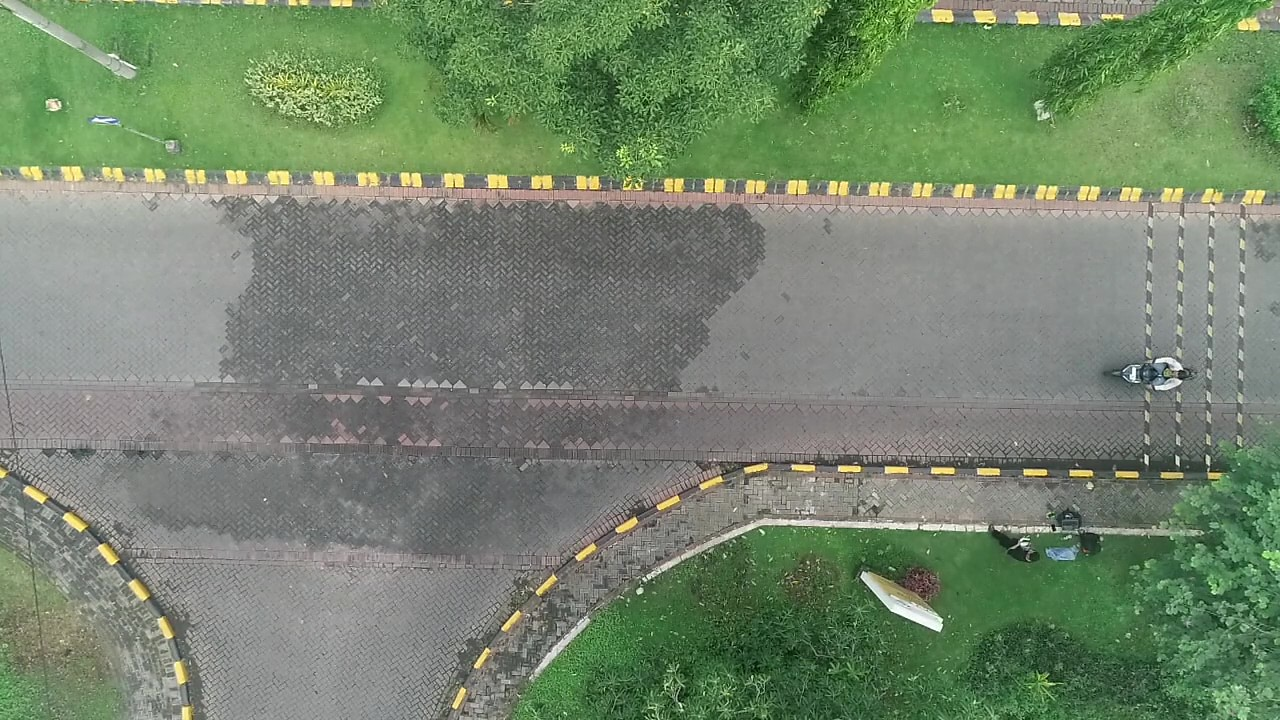
\includegraphics[width=\linewidth]{bab4/20m_siang_40km.jpg}
    \caption{Ketinggian 20 Meter}
    \label{fig:20m_siang_40kmh}
  \end{subfigure}%
  \hfill
  \begin{subfigure}[b]{0.45\textwidth}
    \centering
    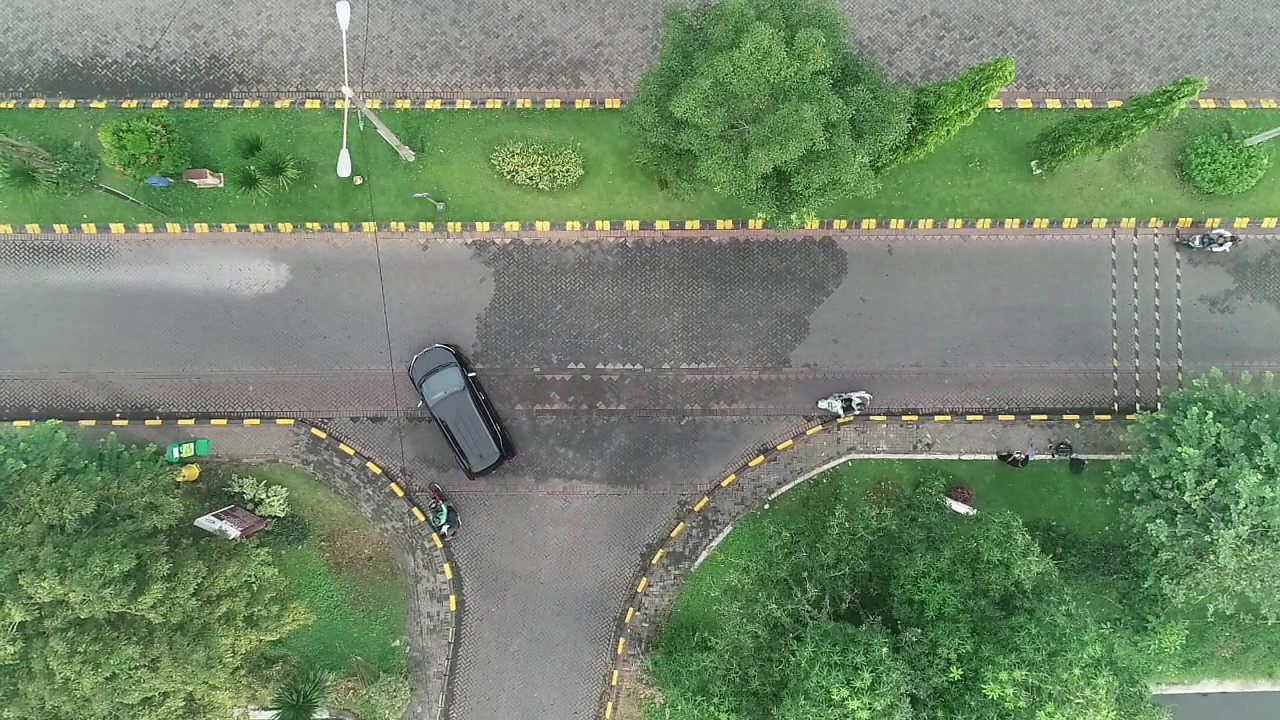
\includegraphics[width=\linewidth]{bab4/30m_siang_40km.jpg}
    \caption{Ketinggian 30 Meter}
    \label{fig:30m_siang_40kmh}
  \end{subfigure}%
  \hfill
  \begin{subfigure}[b]{0.45\textwidth}
    \centering
    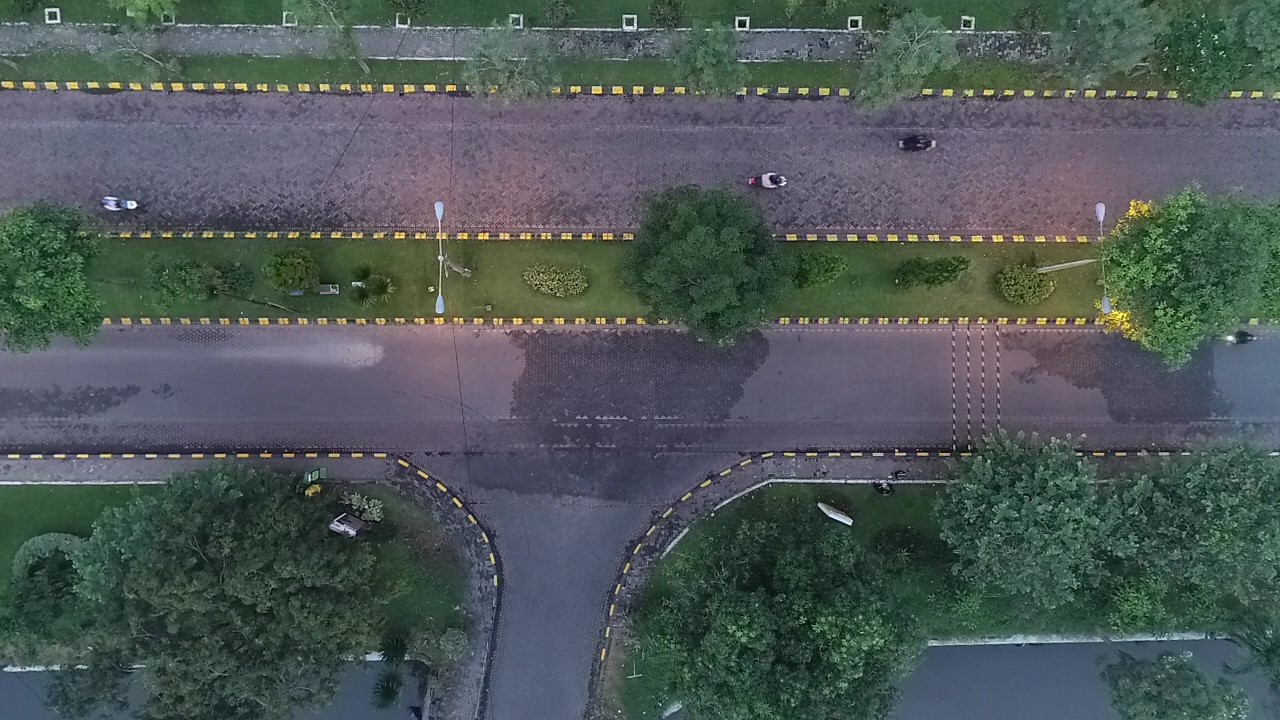
\includegraphics[width=\linewidth]{bab4/40m_siang_40km.jpg}
    \caption{Ketinggian 40 Meter}
    \label{fig:40m_siang_40kmh}
  \end{subfigure}
  \caption{Pengujian Sistem dengan Kecepatan Rata-rata 40km/h pada Siang Hari}
  \label{fig:uji20m_40kmh}
\end{figure}

Kemudian, didapatkan data pengujian sistem dengan kecepatan rata-rata 40km/h, beserta data dari penelitian terdahulu sehingga dapat diketahui seberapa akurat sistem. Hasil data pengujian dan data penelitian terdahulu dapat dilihat pada Tabel \ref{table:40km/h-siang-sistem}, Tabel \ref{table:40km/h-siang-iqbal}, dan Tabel \ref{table:30kmh-sistem-Tilon}.

\begin{table}[H]
	\caption{Pengujian dengan Kecepatan Rata-rata 40km/h pada Siang Hari}
    \label{table:40km/h-siang-sistem}
	\centering
	\begin{tabular}{|c|c|c|c|c|c|}
		\hline
		\multirow{2}{*}{\makecell{\textbf{Ketinggian} \\ \textbf{(Km/h)}}}& \multicolumn{3}{c|}{\textbf{Rata-rata Kecepatan (Km/h)}} & \multirow{2}{*}{\makecell{\textbf{Rata-rata} \\ \textbf{(Km/h)}}} & \multirow{2}{*}{\makecell{\textbf{Standar} \\ \textbf{Deviasi}}} \\ \cline{2-4}
		& 1 & 2 & 3 & \\ \hline
		20 & 37,8 & 36,5 & 43,6 & 39,3 & 3,09\\
		30 & 37,64 & 37,35 & 35,35 & 36,78 & 1,01\\
		40 & 36,58 & 36,64 & 35 & 36,07 & 0,76\\ \hline
	\end{tabular}
\end{table}
\vspace{-10pt}
\begin{table}[H]
	\caption{Pengujian Peneletian \ref{subsec:Iqbal2024} dengan Kecepatan Rata-rata 40km/h pada Siang Hari}
    \label{table:40km/h-siang-iqbal}
	\centering
	\begin{tabular}{|c|c|c|c|c|c|}
		\hline
		\multirow{2}{*}{\makecell{\textbf{Ketinggian} \\ \textbf{(Meter)}}} & \multicolumn{3}{c|}{\textbf{Rata-rata Kecepatan (Km/h)}} & \multirow{2}{*}{\makecell{\textbf{Rata-rata} \\ \textbf{(Km/h)}}} & \multirow{2}{*}{\makecell{\textbf{Standar} \\ \textbf{Deviasi}}} \\ \cline{2-4}
		& 1 & 2 & 3 & \\ \hline
		20 & 35,40 & 37,03 & 35,11 & 35,85 & 1,91 \\ 
		30 & 35,97 & 36,28 & 34,18 & 35,47 & 3,04 \\ 
		40 & 32,89 & 36,13 & 32,98 & 34,00 & 2,50 \\ \hline
	\end{tabular}
\end{table}
\vspace{-10pt}
\begin{table}[H]
	\caption{Pengujian Penelitian \ref{subsec:Tilon2023} dengan Kecepatan Rata-rata 30 km/h}
    \label{table:30kmh-sistem-Tilon}
	\centering
	\begin{tabular}{|c|c|}
		\hline
		\textbf{Ketinggian (Meter)} & \textbf{Kecepatan Prediksi(Km/h)} \\ \hline
		50 & 22,83 \\ \hline
	\end{tabular}
\end{table}

Hasil pengujian pada Tabel \ref{table:40km/h-siang-sistem} menunjukkan standar deviasi tertinggi pada ketinggian 20m sebesar (3.09) yang menandakan terdapat variasi rata-rata dari kecepatan yang dihitung di semua percobaan. Kemudian, pada Penelitian \ref{table:40km/h-siang-iqbal} menunjukkan standar deviasi tertinggi pada ketinggian 30m sebesar (3.04). Apabila dilihat antara hasil pengujian sistem dengan penelitian terdahulu mengalami beberapa variasi dan terdapat \emph{error}, seperti pada Tabel \ref{table:30kmh-sistem-Tilon} terlihat selisih kecepatan hasil pengujiannya dengan hasil perhitungan manual pada Tabel \ref{table:30kmh-manual-Tilon} sekitar 6km/h.

Setelah didapatkan data hasil pengujian, dapat dihitung seberapa besar \emph{error} yang dialami dan tingkat akurasi masing-masing sistem.

\begin{table}[H]
\centering
	\caption{Perhitungan Error dan Akurasi dengan Kecepatan Rata-rata 40Km/h saat Siang Hari pada Percobaan 1}
	\label{table:error_accuracy_per1_40km/h_siang}
	\begin{tabular}{|c|c|c|c|c|}
	\hline
	\textbf{Ketinggian (m)} & \textbf{Error} & \textbf{Absolute Error} & \textbf{Relative Error (\%)} & \textbf{Accuracy (\%)} \\
	\hline
	20 & -2.00 & 2.00 & 5.03 & 94.97 \\
	30 & -1.98 & 1.98 & 5.00 & 95.00 \\
	40 & -3.30 & 3.30 & 8.28 & 91.72 \\
	\hline
	\end{tabular}
\end{table}
\vspace{-10pt}
\begin{table}[H]
\centering
	\caption{Perhitungan Error dan Akurasi dengan Kecepatan Rata-rata 40Km/h saat Siang Hari pada Percobaan 2}
	\label{table:error_accuracy_per2_40km/h_siang}
	\begin{tabular}{|c|c|c|c|c|}
	\hline
	\textbf{Ketinggian (m)} & \textbf{Error} & \textbf{Absolute Error} & \textbf{Relative Error (\%)} & \textbf{Accuracy (\%)} \\
	\hline
	20 & -2.74 & 2.74 & 6.98 & 93.02 \\
	30 & -2.22 & 2.22 & 5.61 & 94.39 \\
	40 & -3.30 & 3.30 & 8.27 & 91.73 \\
	\hline
	\end{tabular}
\end{table}
\vspace{-10pt}
\begin{table}[H]
\centering
	\caption{Perhitungan Error dan Akurasi dengan Kecepatan Rata-rata 40Km/h saat Siang Hari pada Percobaan 3}
	\label{table:error_accuracy_per3_40km/h_siang}
	\begin{tabular}{|c|c|c|c|c|}
	\hline
	\textbf{Ketinggian (m)} & \textbf{Error} & \textbf{Absolute Error} & \textbf{Relative Error (\%)} & \textbf{Accuracy (\%)} \\
	\hline
	20 & 4.20 & 4.20 & 10.66 & 89.34 \\
	30 & -3.17 & 3.17 & 8.23 & 91.77 \\
	40 & -4.64 & 4.64 & 11.71 & 88.29 \\
	\hline
	\end{tabular}
\end{table}
\vspace{-10pt}
Berdasarkan ketiga tabel tersebut dapat dilihat bahwa pada Percobaan 1 (Tabel \ref{table:error_accuracy_per1_40km/h_siang}) nilai \emph{error} berkisar antara –3,30 hingga –2,00 km/h dengan relative \emph{error} tertinggi 8,28\% (pada ketinggian 40 m) dan akurasi minimal 91,72\%. Pada Percobaan 2 (Tabel \ref{table:error_accuracy_per2_40km/h_siang}) memiliki \emph{error} di sekitar –3,30 hingga –2,22 km/h, dan \emph{relative error} tertinggi 8,27\% sehingga akurasi minimal 91,73\%. Sedangkan pada Percobaan 3 (Tabel \ref{table:error_accuracy_per3_40km/h_siang}) terlihat \emph{error} paling variatif, dari 4,20 km/h pada ketinggian 20m hingga –4,64 km/h pada 40m, dengan \emph{relative error} tertinggi 11,71\% dan akurasi terendah 88,29\%. Secara umum, semakin besar ketinggian, semakin besar deviasi hasil sistem terhadap hitungan manual, dan Percobaan 3 menunjukkan fluktuasi error paling signifikan dibanding dua percobaan sebelumnya, yang mengindikasikan kondisi pengukuran, misalnya pencahayaan atau sudut pandang \emph{drone} paling tidak stabil pada saat percobaan ketiga.

\begin{table}[H]
\centering
	\caption{Akurasi pada Penelitian \ref{subsec:Iqbal2024} dengan Kecepatan Rata-rata 40 Km/h saat Siang Hari}
	\label{table:accuracy_40km/h_iqbal}
	\begin{tabular}{|c|c|c|c|}
	\hline
	\textbf{Ketinggian (m)} & \textbf{Percobaan 1 (\%)} & \textbf{Percobaan 2 (\%)} & \textbf{Percobaan 3 (\%)} \\
	\hline
	20 & 89,75 & 90,52 & 88,26 \\
	30 & 93,47 & 91,55 & 87,98 \\
	40 & 86,11 & 94,96 & 89,13 \\
	\hline
	\end{tabular}
\end{table}
\vspace{-10pt}
\begin{table}[H]
\centering
\caption{Akurasi pada Penelitian \ref{subsec:Tilon2023} dengan Kecepatan Rata-rata 30 km/h}
\label{table:accuracy_tilon_30km/h}
\begin{tabular}{|c|c|}
\hline
\textbf{Ketinggian (m)} & \textbf{Percobaan 1 (\%)} \\ \hline
50 & 79,97 \\ \hline
\end{tabular}
\end{table}

Berdasarkan hasil pengujian yang dilakukan serta perbandingan dengan data penelitian terdahulu, beberapa hal yang dapat disimpulkan terkait akurasi pengukuran kecepatan kendaraan menggunakan drone dengan kecepatan rata-rata 40\,km/h pada siang hari adalah sebagai berikut:

\begin{itemize}[nolistsep]
  \item Percobaan 1 mencatat akurasi:
    \begin{itemize}[nolistsep]
      \item Memulai pada 94,97\% di 20\,m,
      \item Meningkat ke puncak 95,05\% di 30\,m,
      \item Menurun menjadi 91,72\% di 40\,m.
    \end{itemize}
  \item Percobaan 2 menunjukkan akurasi relatif stabil dengan:
    \begin{itemize}[nolistsep]
      \item Puncak 94,39\% pada 30\,m,
      \item Terendah 91,73\% pada 40\,m.
    \end{itemize}
  \item Percobaan 3 memiliki variasi akurasi terbesar, yaitu:
    \begin{itemize}[nolistsep]
      \item Memulai pada 89,34\% di 20\,m,
      \item Meningkat ke 91,77\% di 30\,m,
      \item Menurun ke terendah 88,29\% di 40\,m.
    \end{itemize}

  \item Secara keseluruhan, ketinggian 30\,m memberikan hasil pengukuran yang paling akurat dan konsisten pada kecepatan 40\,km/h.

  \item Perbandingan dengan Penelitian Terdahulu
	\begin{itemize}[nolistsep]
	\item Penelitian \ref{subsec:Iqbal2024} (kecepatan rata-rata 40km/h) menunjukkan akurasi berkisar antara 87,98\% hingga 89,13\%, sedikit lebih rendah dan dengan variasi yang lebih besar dibandingkan penelitian ini.
	\item Penelitian \ref{subsec:Tilon2023} (kecepatan rata-rata 30km/h pada ketinggian 50m) hanya mencapai akurasi 79,97\%, menegaskan pengaruh ketinggian dan kecepatan terhadap akurasi.
	\end{itemize}
	\item Beberapa faktor penting yang perlu dipertimbangkan untuk meningkatkan akurasi pengukuran:
	\begin{itemize}[nolistsep]
	\item Perbedaan pengaturan kamera \emph{drone}
	\item Kondisi cuaca
	\item Stabilitas perangkat (device)
	\item Pengaturan kecepatan kendaraan
	\end{itemize}
\end{itemize}
Meskipun yang dilakukan penelitian objek yang sama dan fokus yang sama tetapi terdapat perbedaan hasil dikarenakan kurang sempurnanya sistem dan perbedaan perhitungan yang dilakukan.
\vspace{10ex}
\section{Pengujian Sistem terhadap Kecepatan Rata-rata 20Km/H pada Malam Hari}

Pada pengujian malam hari tepatnya sekitar pukul 00.30 WIB hingga 03.00 WIB, kendaraan motor dikendarai dengan kecepatan rata-rata 20 km/h. Tujuan pengujian ini adalah untuk menguji kinerja sistem pada kondisi pencahayaan yang lebih rendah dan intensitas lalu lintas yang berbeda dibandingkan dengan siang hari. Pengujian dilakukan pada malam hari untuk mengetahui sejauh mana sistem dapat mengestimasi kecepatan dalam kondisi pencahayaan yang terbatas, yang seringkali mengarah pada tantangan lebih besar dalam pengolahan citra dan deteksi objek.
\vspace{-10pt}
\begin{table}[H]
	\caption{Perhitungan Manual dengan Kecepatan Rata-rata 20km/h pada Malam Hari}
    \label{table:20km/h-malam-manual}
	\centering
	\begin{tabular}{|c|c|c|c|c|}
		\hline
		\multirow{2}{*}{\textbf{Ketinggian (Meter)}} & \multicolumn{3}{c|}{\textbf{Rata-rata Kecepatan (Km/h)}} & \multirow{2}{*}{\textbf{Rata-rata (Km/h)}} \\ \cline{2-4}
		& 1 & 2 & 3 & \\ \hline
		20 & 18,82 & 18,68 & 18,75 & 18,75 \\
		30 & 22,45 & 22,28 & 22,52 & 22,42 \\
		40 & 18,97 & 18,73 & 18,59 & 18,76 \\ \hline
	\end{tabular}
\end{table}
\vspace{-10pt}
Pada Tabel \ref{table:20km/h-malam-manual} dapat dilihat perhitungan manual dengan target kecepatan 20km/h yang menghasilkan nilai rata-rata untuk setiap ketinggiannya. Pada ketinggian 30m, terdapat perbedaan yang signifikan dengan ketinggian yang lain, dimana terukur hingga 22,42 km/h untuk rata-ratanya. Hal ini kemungkinan disebabkan karena kesalahan penguji dalam mengukur waktu dan jarak secara benar.

Kemudian, didapatkan hasil pengujian sistem terhadap kecepatan rata-rata 20km/h pada malam hari. Pengujian sistem dilakukan di 3 variasi ketinggian, yang dapat dilihat pada Gambar \ref{fig:ujimalam_20kmh}

\begin{figure}[H]
  \centering
  \begin{subfigure}[b]{0.3\textwidth}
    \centering
    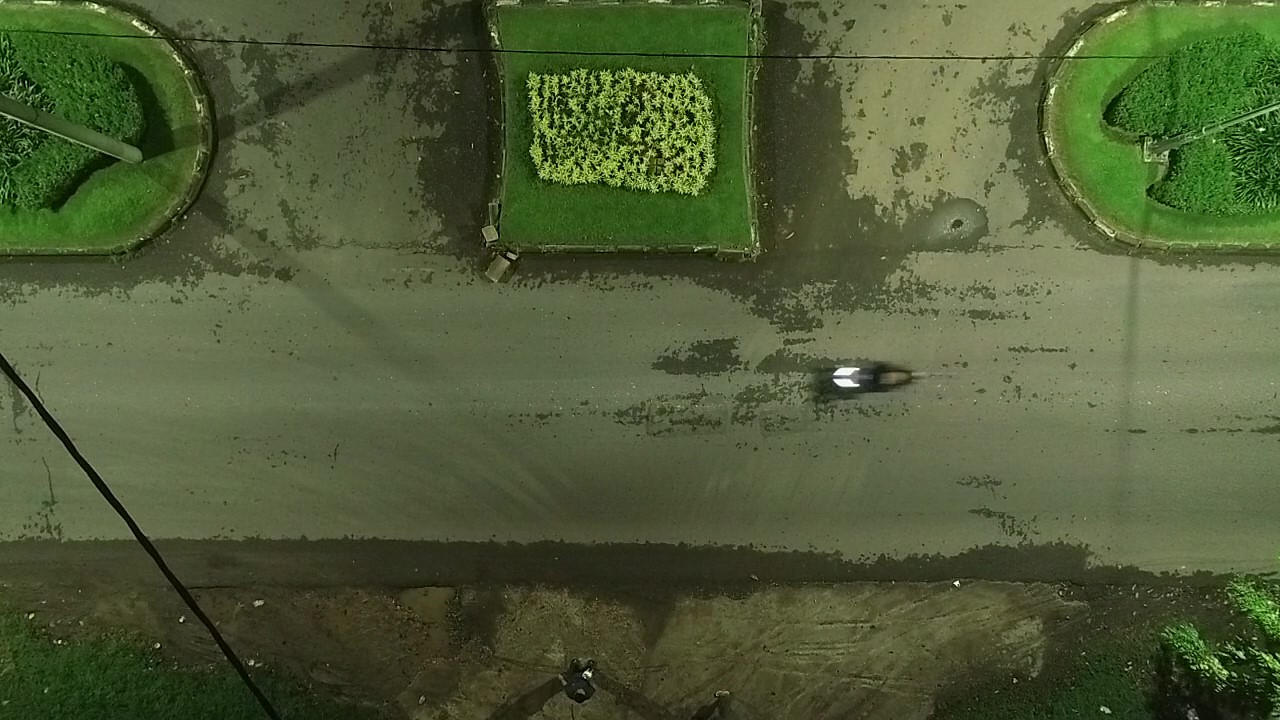
\includegraphics[width=\linewidth]{bab4/20m_malam_20km.jpg}
    \caption{Ketinggian 20 Meter}
    \label{fig:20m_malam_20kmh}
  \end{subfigure}%
  \hfill
  \begin{subfigure}[b]{0.3\textwidth}
    \centering
    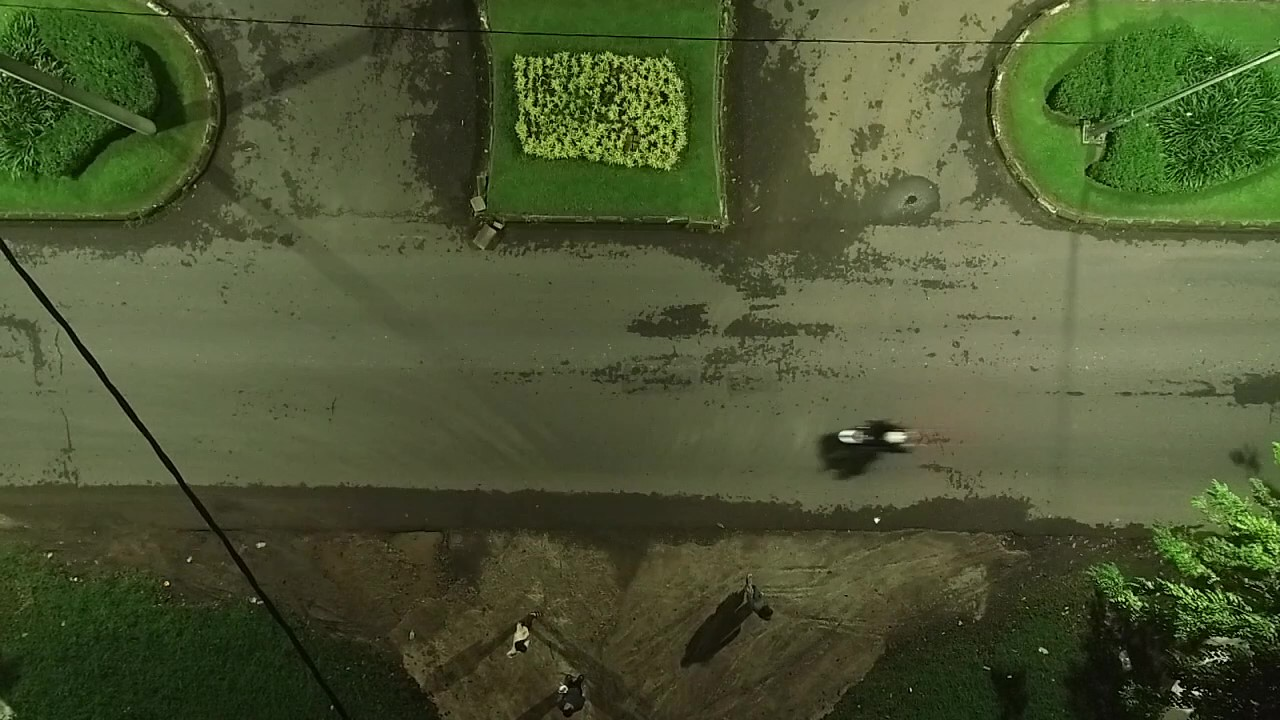
\includegraphics[width=\linewidth]{bab4/30m_malam_20km.jpg}
    \caption{Ketinggian 30 Meter}
    \label{fig:30m_malam_20kmh}
  \end{subfigure}%
  \hfill
  \begin{subfigure}[b]{0.3\textwidth}
    \centering
    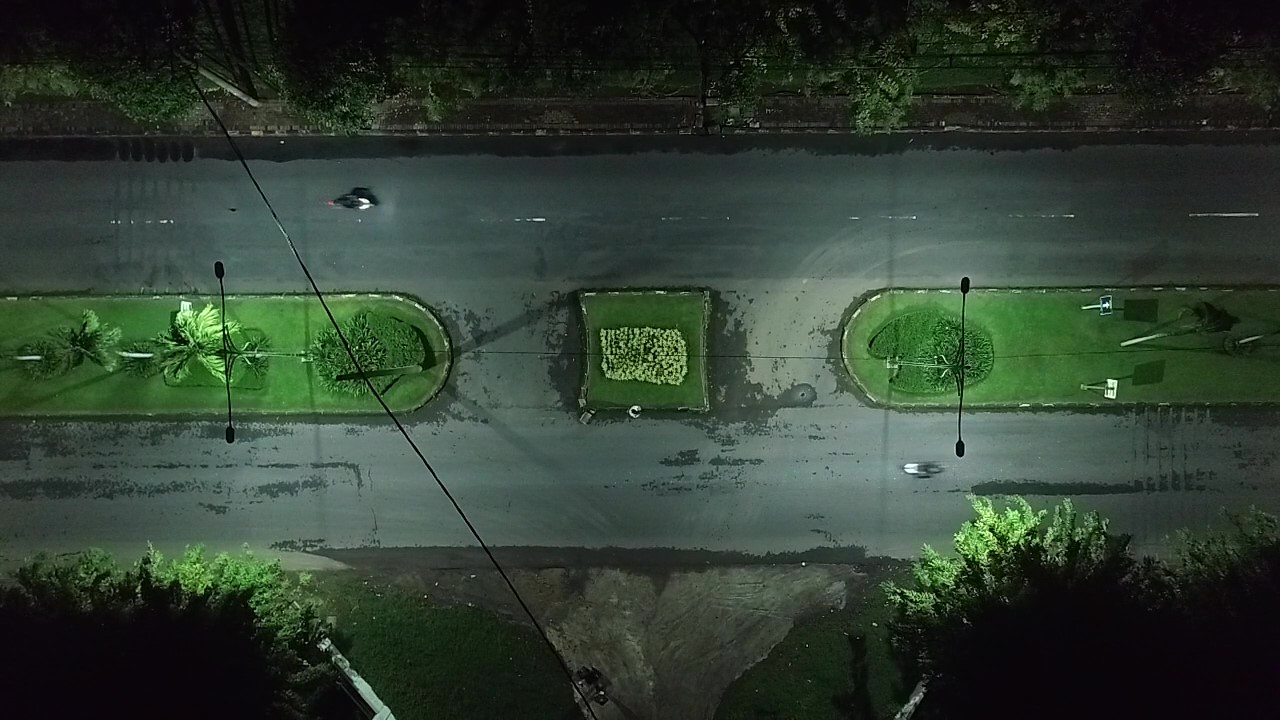
\includegraphics[width=\linewidth]{bab4/40m_malam_20km.jpg}
    \caption{Ketinggian 40 Meter}
    \label{fig:40m_malam_20kmh}
  \end{subfigure}
  \caption{Pengujian Sistem dengan Kecepatan Rata-rata 20km/h pada Malam Hari}
  \label{fig:ujimalam_20kmh}
\end{figure}

Data pengujian didapatkan untuk setiap ketinggian dengan 3 kali percobaan, dengan ditambah adanya nilai standar deviasi untuk mengetahui variasi data.

\begin{table}[H]
	\caption{Pengujian dengan Kecepatan Rata-rata 20km/h pada Malam Hari}
    \label{table:20km/h-malam-sistem}
	\centering
	\begin{tabular}{|c|c|c|c|c|c|}
		\hline
		\multirow{2}{*}{\makecell{\textbf{Ketinggian} \\ \textbf{(Meter)}}}& \multicolumn{3}{c|}{\textbf{Rata-rata Kecepatan (Km/h)}} & \multirow{2}{*}{\makecell{\textbf{Rata-rata} \\ \textbf{(Km/h)}}} & \multirow{2}{*}{\makecell{\textbf{Standar} \\ \textbf{Deviasi}}} \\ \cline{2-4}
		& 1 & 2 & 3 & \\ \hline
		20 & 17,01 & 20,69 & 18,16 & 18,62 & 1,88\\
		30 & 20,88 & 23,17 & 21,32 & 21,79 & 1,22\\
		40 & 24,02 & 22,63 & 21,63 & 22,76 & 1,20\\ \hline
	\end{tabular}
\end{table}
\vspace{-10pt}
Pada Tabel \ref{table:20km/h-malam-sistem} terlihat bahwa semua ketinggian memiliki standar deviasi lebih dari nilai 1. Ketinggian 20 meter memiliki standar deviasi paling tinggi yaitu sebesar 1,88 yang menandakan variasi hasil perhitungan. Ketinggian 40 meter memiliki standar deviasi paling rendah yaitu 1,22 sedangkan ketinggian 30 meter hanya selisih 0,02 daripada ketinggian 40 meter.

Kemudian, dilakukan perhitungan \emph{error} dari hasil pengujian yang telah dilakukan untuk mengetahui seberapa akurat sistem melakukan tugasnya. Perhitungan ini dapat dilihat pada Tabel \ref{tab:20kmh-malam-p1}, \ref{tab:20kmh-malam-p2}, \ref{tab:20kmh-malam-p3}.

\begin{table}[H]
  \caption{Perhitungan Error dan Akurasi dengan Kecepatan Rata-rata 20 km/h saat Malam Hari pada Percobaan 1}
  \label{tab:20kmh-malam-p1}
  \centering
  \begin{tabular}{|c|c|c|c|c|}
    \hline
    \textbf{Ketinggian (m)} & \textbf{Error} & \textbf{Absolute Error} & \textbf{Relative Error (\%)} & \textbf{Accuracy (\%)} \\
    \hline
    20 & \(-1.81\) & 1.81 & 9.62 & 90.38 \\
    30 & \(-1.57\) & 1.57 & 6.99 & 93.01 \\
    40 &  5.05     & 5.05 & 26.63 & 73.37 \\
    \hline
  \end{tabular}
\end{table}
\vspace{-10pt}
\begin{table}[H]
  \caption{Perhitungan Error dan Akurasi dengan Kecepatan Rata-rata 20 km/h saat Malam Hari pada Percobaan 2}
  \label{tab:20kmh-malam-p2}
  \centering
  \begin{tabular}{|c|c|c|c|c|}
    \hline
    \textbf{Ketinggian (m)} & \textbf{Error} & \textbf{Absolute Error} & \textbf{Relative Error (\%)} & \textbf{Accuracy (\%)} \\
    \hline
    20 &  2.01 & 2.01 & 10.77 & 89.23 \\
    30 &  0.89 & 0.89 &  3.99 & 96.01 \\
    40 &  3.90 & 3.90 & 20.83 & 79.17 \\
    \hline
  \end{tabular}
\end{table}
\vspace{-10pt}
\begin{table}[H]
  \caption{Perhitungan Error dan Akurasi dengan Kecepatan Rata-rata 20 km/h saat Malam Hari pada Percobaan 3}
  \label{tab:20kmh-malam-p3}
  \centering
  \begin{tabular}{|c|c|c|c|c|}
    \hline
    \textbf{Ketinggian (m)} & \textbf{Error} & \textbf{Absolute Error} & \textbf{Relative Error (\%)} & \textbf{Accuracy (\%)} \\
    \hline
    20 & \(-0.59\) & 0.59 & 3.15 & 96.85 \\
    30 & \(-1.20\) & 1.20 & 5.33 & 94.67 \\
    40 &  3.04     & 3.04 & 16.36 & 83.64 \\
    \hline
  \end{tabular}
\end{table}

\section{Pengujian Sistem terhadap Kecepatan Rata-rata 40Km/H pada Malam Hari}

Selain pengujian siang hari dengan kecepatan tinggi, pengujian juga dilakukan pada malam hari sekitar pukul 00.30 WIB hingga 03.00 WIB dengan kecepatan kendaraan motor rata-rata 40 km/h. Pengujian ini bertujuan untuk mengevaluasi seberapa baik sistem dapat menangani estimasi kecepatan kendaraan yang lebih cepat meskipun dalam kondisi malam hari dengan pencahayaan yang kurang optimal. Hal ini memberikan gambaran seberapa efektif sistem bekerja di berbagai kondisi, termasuk pada malam hari dengan kecepatan tinggi, yang biasanya membutuhkan performa sistem yang lebih baik dalam mendeteksi dan menghitung kecepatan.

\begin{table}[H]
	\caption{Perhitungan Manual dengan Kecepatan Rata-rata 40km/h pada Malam Hari}
    \label{table:40km/h-malam-manual}
	\centering
	\begin{tabular}{|c|c|c|c|c|}
		\hline
		\multirow{2}{*}{\textbf{Ketinggian (Meter)}} & \multicolumn{3}{c|}{\textbf{Rata-rata Kecepatan (Km/h)}} & \multirow{2}{*}{\textbf{Rata-rata (Km/h)}} \\ \cline{2-4}
		& 1 & 2 & 3 & \\ \hline
		20 & 38,76 & 37,90 & 38,53 & 38,39 \\
		30 & 38,2 & 43,67 & 41,23 & 41,03 \\
		40 & 41,92 & 39,67 & 39,64 & 40,41 \\ \hline
	\end{tabular}
\end{table}
\vspace{-10pt}

Pada Tabel \ref{table:40km/h-malam-manual} dapat diketahui hasil perhitungan manual yang digunakan sebagai referensi dalam menentukan akurasi sistem. Kemudian, titik pengujian yang dilakukan dapat dilihat pada Gambar \ref{fig:ujimalam_40kmh}.
\begin{figure}[H]
  \centering
  \begin{subfigure}[b]{0.3\textwidth}
    \centering
    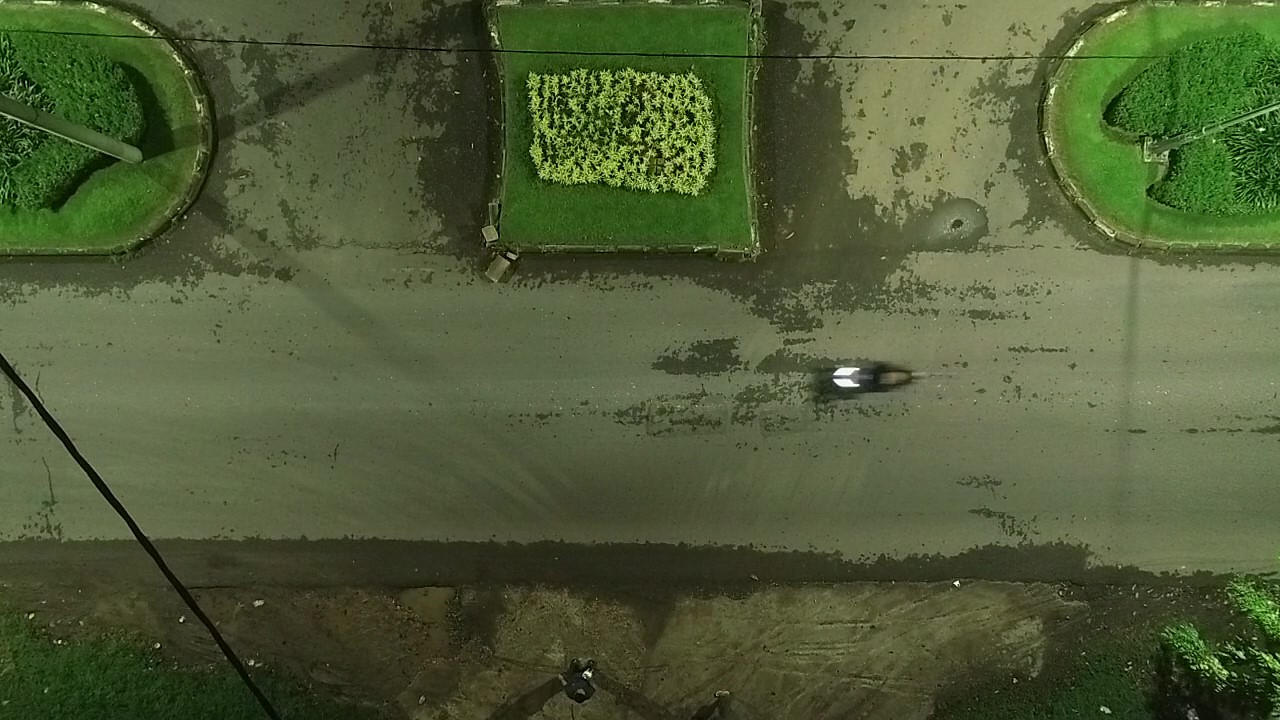
\includegraphics[width=\linewidth]{bab4/20m_malam_20km.jpg}
    \caption{Ketinggian 20 Meter}
    \label{fig:20m_malam_40kmh}
  \end{subfigure}%
  \hfill
  \begin{subfigure}[b]{0.3\textwidth}
    \centering
    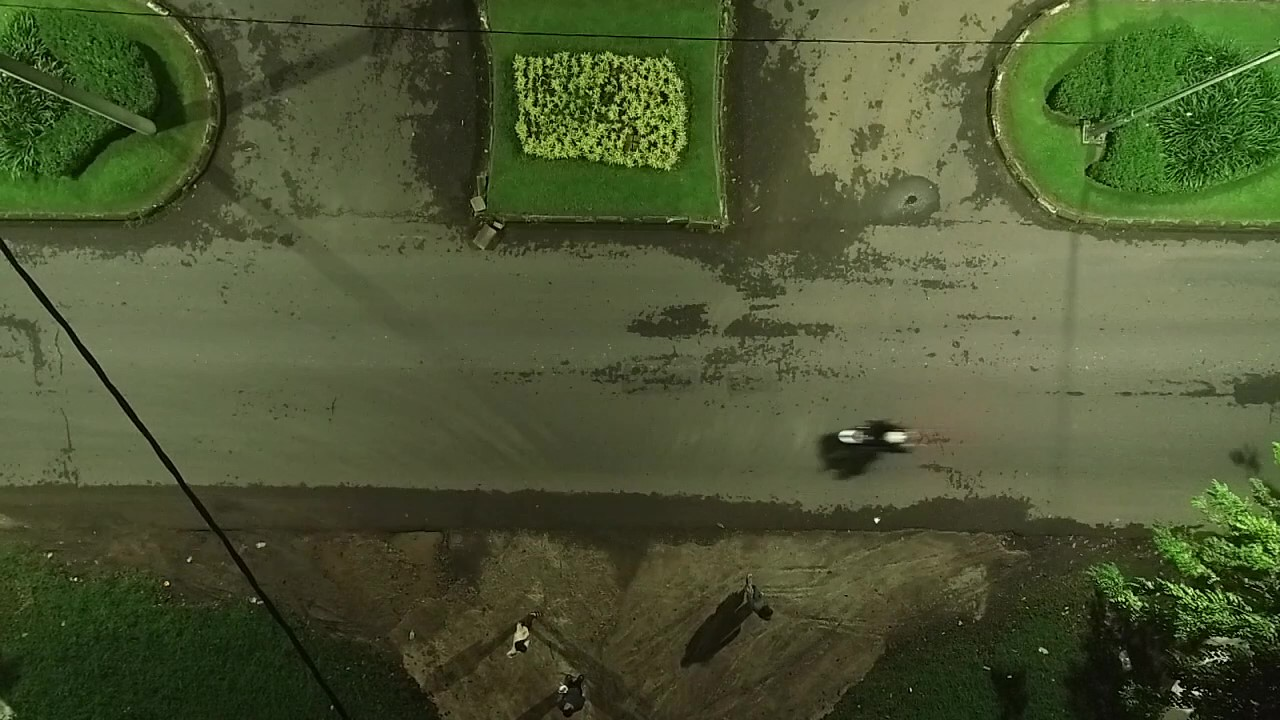
\includegraphics[width=\linewidth]{bab4/30m_malam_20km.jpg}
    \caption{Ketinggian 30 Meter}
    \label{fig:30m_malam_40kmh}
  \end{subfigure}%
  \hfill
  \begin{subfigure}[b]{0.3\textwidth}
    \centering
    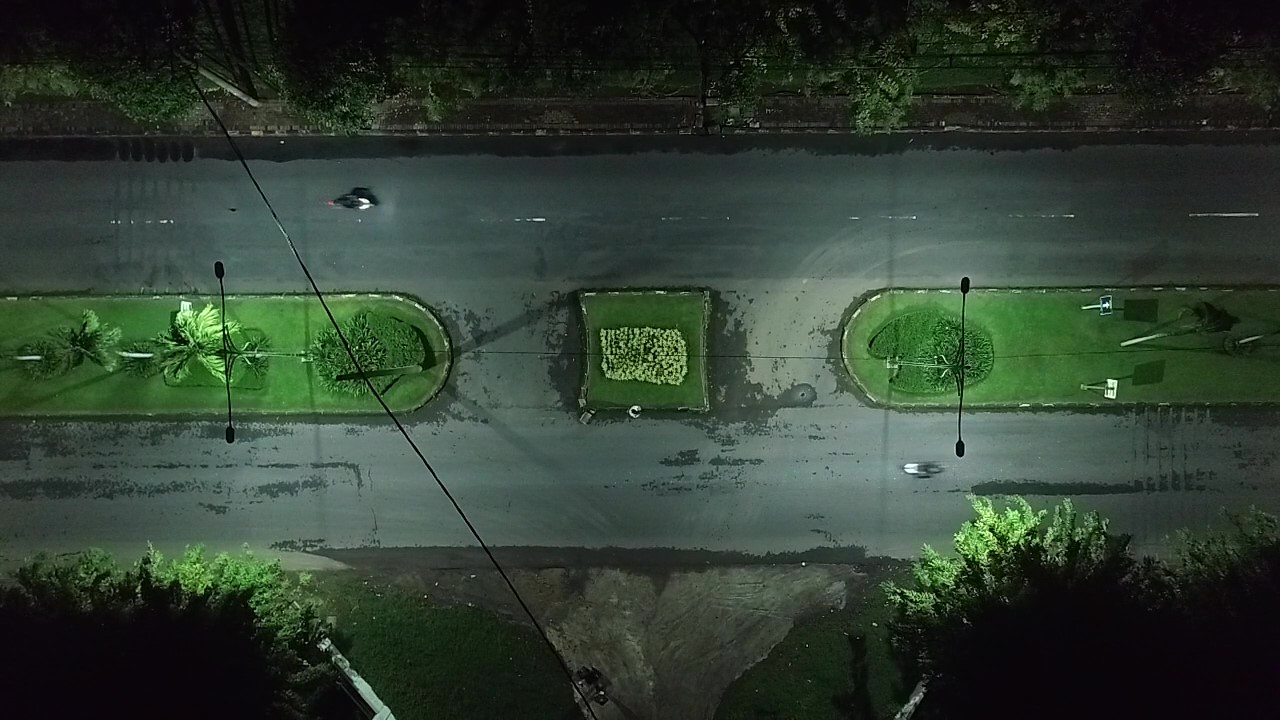
\includegraphics[width=\linewidth]{bab4/40m_malam_20km.jpg}
    \caption{Ketinggian 40 Meter}
    \label{fig:40m_malam_40kmh}
  \end{subfigure}
  \caption{Pengujian Sistem dengan Kecepatan Rata-rata 40km/h pada Malam Hari}
  \label{fig:ujimalam_40kmh}
\end{figure}

\begin{table}[H]
	\caption{Pengujian dengan Kecepatan Rata-rata 40km/h pada Malam Hari}
    \label{table:40km/h-malam-sistem}
	\centering
	\begin{tabular}{|c|c|c|c|c|c|}
		\hline
		\multirow{2}{*}{\makecell{\textbf{Ketinggian} \\ \textbf{(Meter)}}}& \multicolumn{3}{c|}{\textbf{Rata-rata Kecepatan (Km/h)}} & \multirow{2}{*}{\makecell{\textbf{Rata-rata} \\ \textbf{(Km/h)}}} & \multirow{2}{*}{\makecell{\textbf{Standar} \\ \textbf{Deviasi}}} \\ \cline{2-4}
		& 1 & 2 & 3 & \\ \hline
		20 & 39,05 & 38,07 & 45,34 & 40,82 & 3,95 \\
		30 & 40,06 & 33,07 & 33,85 & 35,66 & 3,83 \\
		40 & 40,87 & 38,43 & 42,13 & 40,47 & 1,88 \\ \hline
	\end{tabular}
\end{table}
\vspace{-10pt}

Pada Tabel \ref{table:40km/h-malam-sistem} didapatkan standar deviasi untuk masing-masing ketinggian, yaitu 20m, 30m, dan 40m dengan kecepatan rata-rata 40km/h. Pada ketinggian 20m mengalami variasi rata-rata kecepatan yang variatif sebesar 3,95. Untuk standar deviasi terendah ada di ketinggian 40m sebesar 1,88. Untuk ketinggian 20m dan 30m terdapat selisih sebesar 0,12 dalam standar deviasi yang dimiliki.

Setelah didapatkan hasil pengujian untuk kecepatan rata-rata 40km/h tersebut maka dapat dihitung \emph{error} untuk masing-masing percobaan dan mengetahui seberapa akurasi alat ini.

\begin{table}[H]
  \caption{Perhitungan Error dan Akurasi dengan Kecepatan Rata-rata 40 km/h saat Malam Hari pada Percobaan 1}
  \label{tab:40kmh-malam-p1}
  \centering
  \begin{tabular}{|c|c|c|c|c|}
    \hline
    \textbf{Ketinggian (m)} & \textbf{Error} & \textbf{Absolute Error} & \textbf{Relative Error (\%)} & \textbf{Accuracy (\%)} \\
    \hline
    20 & 0.29  & 0.29 & 0.75 & 99.25 \\
    30 & 1.86  & 1.86 & 4.87 & 95.13 \\
    40 & \(-1.05\) & 1.05 & 2.50 & 97.50 \\
    \hline
  \end{tabular}
\end{table}
\vspace{-10pt}
\begin{table}[H]
  \caption{Perhitungan Error dan Akurasi dengan Kecepatan Rata-rata 40 km/h saat Malam Hari pada Percobaan 2}
  \label{tab:40kmh-malam-p2}
  \centering
  \begin{tabular}{|c|c|c|c|c|}
    \hline
    \textbf{Ketinggian (m)} & \textbf{Error} & \textbf{Absolute Error} & \textbf{Relative Error (\%)} & \textbf{Accuracy (\%)} \\
    \hline
    20 & 0.17  & 0.17 & 0.45 & 99.55 \\
    30 & \(-10.60\) & 10.60 & 24.28 & 75.72 \\
    40 & \(-1.24\) & 1.24 & 3.13 & 96.87 \\
    \hline
  \end{tabular}
\end{table}
\vspace{-10pt}
\begin{table}[H]
  \caption{Perhitungan Error dan Akurasi dengan Kecepatan Rata-rata 40 km/h saat Malam Hari pada Percobaan 3}
  \label{tab:40kmh-malam-p3}
  \centering
  \begin{tabular}{|c|c|c|c|c|}
    \hline
    \textbf{Ketinggian (m)} & \textbf{Error} & \textbf{Absolute Error} & \textbf{Relative Error (\%)} & \textbf{Accuracy (\%)} \\
    \hline
    20 & 6.81  & 6.81 & 17.68 & 82.32 \\
    30 & \(-7.38\) & 7.38 & 17.90 & 82.10 \\
    40 & 2.49  & 2.49 & 6.28 & 93.72 \\
    \hline
  \end{tabular}
\end{table}

\section{Analisis dan Perbandingan terhadap Kualitas Sistem}
Sistem yang dikembangkan pada penelitian ini memanfaatkan modul Jetson Nano untuk menjalankan model YOLOv8 dengan algoritma pelacakan \emph{OCSORT}, dan memanfaatkan \emph{RTMP} sebagai protokol untuk mengirim video dari DJI Phantom 4 Pro ke Jetson Nano. Pengujian menunjukkan bahwa laju frame rate berkisar antara 8–13 \emph{FPS}, di mana nilai tertinggi terjadi pada kondisi kepadatan objek rendah dan menurun mendekati 8 fps saat kepadatan meningkat. Selain beban inferensi dan pelacakan, \emph{delay} pada \emph{streaming} RTMP turut memengaruhi kinerja, karena Jetson Nano harus mengeksekusi penerimaan data, deteksi objek, dan pelacakan secara bersamaan di Jetson Nano yang relatif terbatas sumber dayanya meskipun sudah ditambahkan algoritma \emph{threading} untuk penerimaan data \emph{streaming}nya. Variasi \emph{frame rate} tersebut mengindikasikan adanya batasan memori dan \emph{bandwidth} internal perangkat, sehingga diperlukan optimasi lebih lanjut pada \emph{pipeline} \emph{streaming} atau kompresi data sebelum inferensi untuk mencapai kestabilan kinerja.

Dalam penelitian sebelumnya, Penelitian \ref{subsec:Iqbal2024} melakukan deteksi dan pelacakan objek menggunakan YOLOv8 yang dipadukan dengan \emph{BOTSORT} dan \emph{ByteTrack} pada komputer desktop, di mana data dikirim dari drone melalui antarmuka \emph{Streamlit}. Konfigurasi tersebut menghasilkan kestabilan, namun mketergantungan pada koneksi jaringan eksternal. Sementara itu, Penelitian \ref{subsec:Tilon2023} menerapkan YOLOv4 dengan \emph{SEGMENTATION-INITIALISED TRACKERS} pada platform Jetson Xavier NX dan melaporkan \emph{frame rate} stabil sekitar 8 fps. Hasil ini menunjukkan bahwa meski Xavier NX memiliki kemampuan \emph{GPU} lebih kuat, metode YOLOv8-\emph{OCSORT} yang dijalankan pada Jetson Nano tetap mampu mencapai \emph{throughput} lebih tinggi dalam kondisi ideal, asalkan \emph{optimasi} aliran data dan inferensi dapat diminimalkan latensinya.


\cleardoublepage
\begin{spacing}{1.2}
	\chapter{PENUTUP}
	\label{sec:chap5_penutup}
\end{spacing}
\vspace{4ex}

\section{Kesimpulan}
\label{sec:sec4_kesimpulan}
\vspace{1ex}
Berdasarkan hasil pengujian dan analisis yang telah dilakukan didapatkan beberapa kesimpulan, antara lain:
\begin{enumerate}
    \item Sistem estimasi kecepatan telah berhasil menjalankan deteksi objeknya dengan \emph{confidence threshold} diatas 0,5 untuk setiap \emph{class}, yaitu motor, mobil, dan truk.
    \item \emph{Tracking} masih dapat disempurnakan lagi atau menggunakan metode yang lain sehingga \emph{bounding box} tetap menempel terus pada objek deteksi.
    \item Sistem lebih optimal saat dijalankan di ketinggian 20m. Untuk 30m dan 40m sebenarnya bisa lebih optimal tetapi terhalang dengan spesifikasi perangkat dan juga metode deteksi (YOLOv8) yang digunakan cukup memakan memori.
    \item Deteksi malam hari berhasil dengan pencahayaan yang minimal tetapi perlu disempurnakan di bagian \emph{tracking}.
    \item Akurasi terendah didapatkan saat pengujian kecepatan 20km/h pada siang hari dengan ketinggian 30m. Untuk akurasi tertinggi diperoleh saat pengujian malam hari dengan ketinggian 20m, kecepatan 40km/h.
    \item Sistem ini dapat berjalan dimana saja dan mampu mendapatkan data nya di saat itu juga meskipun ada \emph{delay}. Implementasinya hanya memerlukan laptop, \emph{handphone}, dan internet yang tidak menguras kuota banyak saat menjalankan server satu jaringan. Tetapi, tidak bisa dijalankan terlalu lama karena terhalang perangkat komputasinya, Jetson Nano
\end{enumerate}
\section{Saran}
\label{sec:sec4_saran}
\vspace{1ex}
\begin{enumerate}
    \item Model deteksi harus diperbaiki lagi karena masih bisa disempurnakan melalui variasi akuisisi data.
    \item Menggunakan metode yang lebih ringan daripada YOLOv8 karena Jetson Nano sebenarnya sudah tidak terlalu kompatibel dengan Ultralytics versi 8 keatas.
    \item Dibutuhkan sistem pengiriman data atau \emph{streaming} yang lebih baik lagi dan mendukung untuk perangkat dengan spesifikasi rendah.
    \item Diperlukan pengujian yang lebih siap dan matang supaya tidak terjadi ketimpangan yang tidak diharapkan
\end{enumerate}


\cleardoublepage


\bibliographystyle{unsrt}
\renewcommand{\bibname}{DAFTAR PUSTAKA}
\addcontentsline{toc}{chapter}{DAFTAR PUSTAKA}

\vspace{2ex}
\bibliography{pustaka/pustaka.bib}
\newpage
\cleardoublepage
\begin{center}
  \Large
  \textbf{BIOGRAFI PENULIS}
\end{center}

\addcontentsline{toc}{chapter}{BIOGRAFI PENULIS}

\vspace{2ex}

\begin{wrapfigure}{L}{0.3\textwidth}
  \centering
  \vspace{-3ex}
  % Ubah file gambar berikut dengan file foto dari mahasiswa
  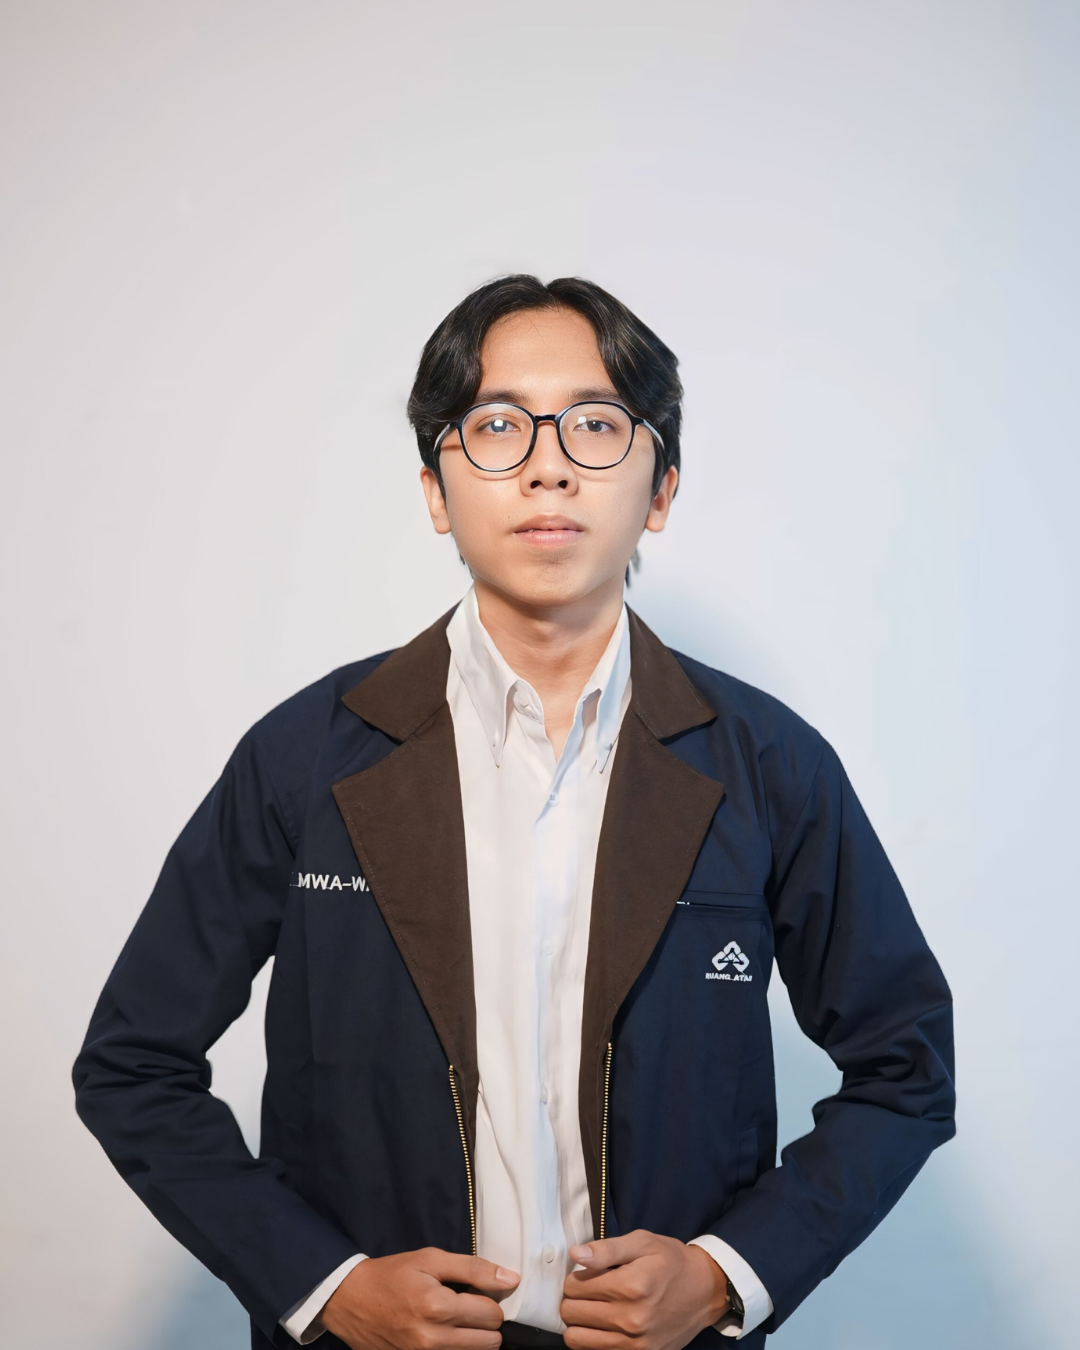
\includegraphics[width=0.3\textwidth]{BiografiPenulis/fotoku.png}
  \vspace{-4ex}
\end{wrapfigure}

% Ubah kalimat berikut dengan biografi dari mahasiswa
\name{}, lahir di Surabaya pada 11 Juni 2003. Setelah menamatkan pendidikan SMA pada tahun 2021. Melanjutkan pendidikan kuliah S-1 di Institut Teknologi Sepuluh Nopember Surabaya, Jurusan Teknik Komputer. Selain kuliah, penulis sering mengikuti kepanitiaan dan organisasi kampus. Minat terhadap pengembangan teknologi yang membuat penulis terpikirkan untuk kuliah di Teknik Komputer. Selain teknologi, manajemen dan bisnis merupakan minat lain yang sedang ditekuni.

Pembaca yang memiliki saran dan kritik terkait penelitian ini dapat menghubungi email syahrulfa1106@gmail.com

\cleardoublepage
\end{document}
